\documentclass[tikz,border=5pt,multi=tikzpicture]{standalone}
\usepackage[UTF8]{ctex}
\usepackage{amsmath}
\usetikzlibrary{arrows.meta,calc}
\definecolor{ink}{HTML}{17365D}
\definecolor{field}{HTML}{287DA8}
\definecolor{force}{HTML}{C56B2A}
\tikzset{every node/.style={font=\small},vec/.style={-{Stealth[length=2mm]},thick},helper/.style={gray,dashed}}
\newcommand{\axisray}{
  \draw[helper] (-.2,0)--(10.3,0);
  \draw[field,thick] (0,-.9)--(0,1.1);\draw[field,thick] (10,-.9)--(10,1.1);
  \fill (2,0) circle (1.1pt) node[below] {$F$};\fill (8,0) circle (1.1pt) node[above] {$F'$};
  \node[below left] at (0,0) {$O$};\node[above right,yshift=4pt] at (10,0) {$O'$};
}
\begin{document}
\begin{tikzpicture}
  \filldraw[ink!40,fill=field!3,thin] (0,0) ellipse (2.71889 and 2.2);
  % Explicit prolate spheroid projection, a=5 b=4.
\draw[gray!60,line width=.35pt] (2.66268,0.00000)--(2.67143,0.04268);
\draw[gray!60,line width=.35pt] (2.67143,0.04268)--(2.67835,0.08534);
\draw[gray!60,line width=.35pt] (2.67835,0.08534)--(2.68344,0.12793);
\draw[gray!60,line width=.35pt] (2.68344,0.12793)--(2.68668,0.17044);
\draw[gray!60,line width=.35pt] (2.68668,0.17044)--(2.68809,0.21283);
\draw[gray!60,line width=.35pt] (2.68809,0.21283)--(2.68765,0.25508);
\draw[gray!60,line width=.35pt] (2.68765,0.25508)--(2.68538,0.29715);
\draw[gray!60,line width=.35pt] (2.68538,0.29715)--(2.68126,0.33902);
\draw[gray!60,line width=.35pt] (2.68126,0.33902)--(2.67530,0.38065);
\draw[gray!60,line width=.35pt] (2.67530,0.38065)--(2.66751,0.42202);
\draw[gray!60,line width=.35pt] (2.66751,0.42202)--(2.65789,0.46311);
\draw[gray!45,dashed,line width=.25pt] (2.65789,0.46311)--(2.64645,0.50388);
\draw[gray!45,dashed,line width=.25pt] (2.64645,0.50388)--(2.63320,0.54430);
\draw[gray!45,dashed,line width=.25pt] (2.63320,0.54430)--(2.61814,0.58435);
\draw[gray!45,dashed,line width=.25pt] (2.61814,0.58435)--(2.60129,0.62399);
\draw[gray!45,dashed,line width=.25pt] (2.60129,0.62399)--(2.58265,0.66321);
\draw[gray!45,dashed,line width=.25pt] (2.58265,0.66321)--(2.56225,0.70198);
\draw[gray!45,dashed,line width=.25pt] (2.56225,0.70198)--(2.54009,0.74027);
\draw[gray!45,dashed,line width=.25pt] (2.54009,0.74027)--(2.51618,0.77804);
\draw[gray!45,dashed,line width=.25pt] (2.51618,0.77804)--(2.49056,0.81529);
\draw[gray!45,dashed,line width=.25pt] (2.49056,0.81529)--(2.46322,0.85197);
\draw[gray!45,dashed,line width=.25pt] (2.46322,0.85197)--(2.43420,0.88807);
\draw[gray!45,dashed,line width=.25pt] (2.43420,0.88807)--(2.40351,0.92357);
\draw[gray!45,dashed,line width=.25pt] (2.40351,0.92357)--(2.37117,0.95843);
\draw[gray!45,dashed,line width=.25pt] (2.37117,0.95843)--(2.33721,0.99263);
\draw[gray!45,dashed,line width=.25pt] (2.33721,0.99263)--(2.30165,1.02615);
\draw[gray!45,dashed,line width=.25pt] (2.30165,1.02615)--(2.26451,1.05897);
\draw[gray!45,dashed,line width=.25pt] (2.26451,1.05897)--(2.22581,1.09107);
\draw[gray!45,dashed,line width=.25pt] (2.22581,1.09107)--(2.18559,1.12241);
\draw[gray!45,dashed,line width=.25pt] (2.18559,1.12241)--(2.14388,1.15299);
\draw[gray!45,dashed,line width=.25pt] (2.14388,1.15299)--(2.10069,1.18278);
\draw[gray!45,dashed,line width=.25pt] (2.10069,1.18278)--(2.05607,1.21175);
\draw[gray!45,dashed,line width=.25pt] (2.05607,1.21175)--(2.01003,1.23990);
\draw[gray!45,dashed,line width=.25pt] (2.01003,1.23990)--(1.96262,1.26719);
\draw[gray!45,dashed,line width=.25pt] (1.96262,1.26719)--(1.91386,1.29362);
\draw[gray!45,dashed,line width=.25pt] (1.91386,1.29362)--(1.86379,1.31916);
\draw[gray!45,dashed,line width=.25pt] (1.86379,1.31916)--(1.81244,1.34380);
\draw[gray!45,dashed,line width=.25pt] (1.81244,1.34380)--(1.75985,1.36751);
\draw[gray!45,dashed,line width=.25pt] (1.75985,1.36751)--(1.70606,1.39029);
\draw[gray!45,dashed,line width=.25pt] (1.70606,1.39029)--(1.65110,1.41212);
\draw[gray!45,dashed,line width=.25pt] (1.65110,1.41212)--(1.59500,1.43298);
\draw[gray!45,dashed,line width=.25pt] (1.59500,1.43298)--(1.53781,1.45285);
\draw[gray!45,dashed,line width=.25pt] (1.53781,1.45285)--(1.47957,1.47173);
\draw[gray!45,dashed,line width=.25pt] (1.47957,1.47173)--(1.42031,1.48960);
\draw[gray!45,dashed,line width=.25pt] (1.42031,1.48960)--(1.36008,1.50645);
\draw[gray!45,dashed,line width=.25pt] (1.36008,1.50645)--(1.29892,1.52227);
\draw[gray!45,dashed,line width=.25pt] (1.29892,1.52227)--(1.23687,1.53705);
\draw[gray!45,dashed,line width=.25pt] (1.23687,1.53705)--(1.17397,1.55077);
\draw[gray!45,dashed,line width=.25pt] (1.17397,1.55077)--(1.11026,1.56343);
\draw[gray!45,dashed,line width=.25pt] (1.11026,1.56343)--(1.04579,1.57501);
\draw[gray!45,dashed,line width=.25pt] (1.04579,1.57501)--(0.98061,1.58552);
\draw[gray!45,dashed,line width=.25pt] (0.98061,1.58552)--(0.91476,1.59494);
\draw[gray!45,dashed,line width=.25pt] (0.91476,1.59494)--(0.84828,1.60327);
\draw[gray!45,dashed,line width=.25pt] (0.84828,1.60327)--(0.78121,1.61050);
\draw[gray!45,dashed,line width=.25pt] (0.78121,1.61050)--(0.71361,1.61662);
\draw[gray!45,dashed,line width=.25pt] (0.71361,1.61662)--(0.64553,1.62164);
\draw[gray!45,dashed,line width=.25pt] (0.64553,1.62164)--(0.57700,1.62555);
\draw[gray!45,dashed,line width=.25pt] (0.57700,1.62555)--(0.50807,1.62834);
\draw[gray!45,dashed,line width=.25pt] (0.50807,1.62834)--(0.43880,1.63002);
\draw[gray!45,dashed,line width=.25pt] (0.43880,1.63002)--(0.36922,1.63057);
\draw[gray!45,dashed,line width=.25pt] (0.36922,1.63057)--(0.29940,1.63002);
\draw[gray!45,dashed,line width=.25pt] (0.29940,1.63002)--(0.22936,1.62834);
\draw[gray!45,dashed,line width=.25pt] (0.22936,1.62834)--(0.15918,1.62555);
\draw[gray!45,dashed,line width=.25pt] (0.15918,1.62555)--(0.08888,1.62164);
\draw[gray!45,dashed,line width=.25pt] (0.08888,1.62164)--(0.01852,1.61662);
\draw[gray!45,dashed,line width=.25pt] (0.01852,1.61662)--(-0.05186,1.61050);
\draw[gray!45,dashed,line width=.25pt] (-0.05186,1.61050)--(-0.12219,1.60327);
\draw[gray!45,dashed,line width=.25pt] (-0.12219,1.60327)--(-0.19245,1.59494);
\draw[gray!45,dashed,line width=.25pt] (-0.19245,1.59494)--(-0.26257,1.58552);
\draw[gray!45,dashed,line width=.25pt] (-0.26257,1.58552)--(-0.33251,1.57501);
\draw[gray!45,dashed,line width=.25pt] (-0.33251,1.57501)--(-0.40222,1.56343);
\draw[gray!45,dashed,line width=.25pt] (-0.40222,1.56343)--(-0.47166,1.55077);
\draw[gray!45,dashed,line width=.25pt] (-0.47166,1.55077)--(-0.54077,1.53705);
\draw[gray!45,dashed,line width=.25pt] (-0.54077,1.53705)--(-0.60952,1.52227);
\draw[gray!45,dashed,line width=.25pt] (-0.60952,1.52227)--(-0.67784,1.50645);
\draw[gray!45,dashed,line width=.25pt] (-0.67784,1.50645)--(-0.74570,1.48960);
\draw[gray!45,dashed,line width=.25pt] (-0.74570,1.48960)--(-0.81306,1.47173);
\draw[gray!45,dashed,line width=.25pt] (-0.81306,1.47173)--(-0.87985,1.45285);
\draw[gray!45,dashed,line width=.25pt] (-0.87985,1.45285)--(-0.94604,1.43298);
\draw[gray!45,dashed,line width=.25pt] (-0.94604,1.43298)--(-1.01158,1.41212);
\draw[gray!45,dashed,line width=.25pt] (-1.01158,1.41212)--(-1.07643,1.39029);
\draw[gray!45,dashed,line width=.25pt] (-1.07643,1.39029)--(-1.14054,1.36751);
\draw[gray!45,dashed,line width=.25pt] (-1.14054,1.36751)--(-1.20387,1.34380);
\draw[gray!45,dashed,line width=.25pt] (-1.20387,1.34380)--(-1.26637,1.31916);
\draw[gray!45,dashed,line width=.25pt] (-1.26637,1.31916)--(-1.32801,1.29362);
\draw[gray!45,dashed,line width=.25pt] (-1.32801,1.29362)--(-1.38874,1.26719);
\draw[gray!45,dashed,line width=.25pt] (-1.38874,1.26719)--(-1.44851,1.23990);
\draw[gray!45,dashed,line width=.25pt] (-1.44851,1.23990)--(-1.50729,1.21175);
\draw[gray!45,dashed,line width=.25pt] (-1.50729,1.21175)--(-1.56504,1.18278);
\draw[gray!45,dashed,line width=.25pt] (-1.56504,1.18278)--(-1.62172,1.15299);
\draw[gray!45,dashed,line width=.25pt] (-1.62172,1.15299)--(-1.67728,1.12241);
\draw[gray!45,dashed,line width=.25pt] (-1.67728,1.12241)--(-1.73169,1.09107);
\draw[gray!45,dashed,line width=.25pt] (-1.73169,1.09107)--(-1.78492,1.05897);
\draw[gray!45,dashed,line width=.25pt] (-1.78492,1.05897)--(-1.83693,1.02615);
\draw[gray!45,dashed,line width=.25pt] (-1.83693,1.02615)--(-1.88767,0.99263);
\draw[gray!45,dashed,line width=.25pt] (-1.88767,0.99263)--(-1.93713,0.95843);
\draw[gray!45,dashed,line width=.25pt] (-1.93713,0.95843)--(-1.98525,0.92357);
\draw[gray!45,dashed,line width=.25pt] (-1.98525,0.92357)--(-2.03201,0.88807);
\draw[gray!45,dashed,line width=.25pt] (-2.03201,0.88807)--(-2.07739,0.85197);
\draw[gray!45,dashed,line width=.25pt] (-2.07739,0.85197)--(-2.12133,0.81529);
\draw[gray!45,dashed,line width=.25pt] (-2.12133,0.81529)--(-2.16383,0.77804);
\draw[gray!45,dashed,line width=.25pt] (-2.16383,0.77804)--(-2.20484,0.74027);
\draw[gray!45,dashed,line width=.25pt] (-2.20484,0.74027)--(-2.24434,0.70198);
\draw[gray!45,dashed,line width=.25pt] (-2.24434,0.70198)--(-2.28230,0.66321);
\draw[gray!45,dashed,line width=.25pt] (-2.28230,0.66321)--(-2.31870,0.62399);
\draw[gray!45,dashed,line width=.25pt] (-2.31870,0.62399)--(-2.35350,0.58435);
\draw[gray!45,dashed,line width=.25pt] (-2.35350,0.58435)--(-2.38670,0.54430);
\draw[gray!45,dashed,line width=.25pt] (-2.38670,0.54430)--(-2.41826,0.50388);
\draw[gray!45,dashed,line width=.25pt] (-2.41826,0.50388)--(-2.44816,0.46311);
\draw[gray!45,dashed,line width=.25pt] (-2.44816,0.46311)--(-2.47639,0.42202);
\draw[gray!45,dashed,line width=.25pt] (-2.47639,0.42202)--(-2.50291,0.38065);
\draw[gray!45,dashed,line width=.25pt] (-2.50291,0.38065)--(-2.52772,0.33902);
\draw[gray!45,dashed,line width=.25pt] (-2.52772,0.33902)--(-2.55080,0.29715);
\draw[gray!45,dashed,line width=.25pt] (-2.55080,0.29715)--(-2.57213,0.25508);
\draw[gray!45,dashed,line width=.25pt] (-2.57213,0.25508)--(-2.59170,0.21283);
\draw[gray!45,dashed,line width=.25pt] (-2.59170,0.21283)--(-2.60950,0.17044);
\draw[gray!45,dashed,line width=.25pt] (-2.60950,0.17044)--(-2.62550,0.12793);
\draw[gray!45,dashed,line width=.25pt] (-2.62550,0.12793)--(-2.63970,0.08534);
\draw[gray!45,dashed,line width=.25pt] (-2.63970,0.08534)--(-2.65210,0.04268);
\draw[gray!45,dashed,line width=.25pt] (-2.65210,0.04268)--(-2.66268,0.00000);
\draw[gray!45,dashed,line width=.25pt] (-2.66268,0.00000)--(-2.67143,-0.04268);
\draw[gray!45,dashed,line width=.25pt] (-2.67143,-0.04268)--(-2.67835,-0.08534);
\draw[gray!45,dashed,line width=.25pt] (-2.67835,-0.08534)--(-2.68344,-0.12793);
\draw[gray!45,dashed,line width=.25pt] (-2.68344,-0.12793)--(-2.68668,-0.17044);
\draw[gray!45,dashed,line width=.25pt] (-2.68668,-0.17044)--(-2.68809,-0.21283);
\draw[gray!45,dashed,line width=.25pt] (-2.68809,-0.21283)--(-2.68765,-0.25508);
\draw[gray!45,dashed,line width=.25pt] (-2.68765,-0.25508)--(-2.68538,-0.29715);
\draw[gray!45,dashed,line width=.25pt] (-2.68538,-0.29715)--(-2.68126,-0.33902);
\draw[gray!45,dashed,line width=.25pt] (-2.68126,-0.33902)--(-2.67530,-0.38065);
\draw[gray!45,dashed,line width=.25pt] (-2.67530,-0.38065)--(-2.66751,-0.42202);
\draw[gray!45,dashed,line width=.25pt] (-2.66751,-0.42202)--(-2.65789,-0.46311);
\draw[gray!60,line width=.35pt] (-2.65789,-0.46311)--(-2.64645,-0.50388);
\draw[gray!60,line width=.35pt] (-2.64645,-0.50388)--(-2.63320,-0.54430);
\draw[gray!60,line width=.35pt] (-2.63320,-0.54430)--(-2.61814,-0.58435);
\draw[gray!60,line width=.35pt] (-2.61814,-0.58435)--(-2.60129,-0.62399);
\draw[gray!60,line width=.35pt] (-2.60129,-0.62399)--(-2.58265,-0.66321);
\draw[gray!60,line width=.35pt] (-2.58265,-0.66321)--(-2.56225,-0.70198);
\draw[gray!60,line width=.35pt] (-2.56225,-0.70198)--(-2.54009,-0.74027);
\draw[gray!60,line width=.35pt] (-2.54009,-0.74027)--(-2.51618,-0.77804);
\draw[gray!60,line width=.35pt] (-2.51618,-0.77804)--(-2.49056,-0.81529);
\draw[gray!60,line width=.35pt] (-2.49056,-0.81529)--(-2.46322,-0.85197);
\draw[gray!60,line width=.35pt] (-2.46322,-0.85197)--(-2.43420,-0.88807);
\draw[gray!60,line width=.35pt] (-2.43420,-0.88807)--(-2.40351,-0.92357);
\draw[gray!60,line width=.35pt] (-2.40351,-0.92357)--(-2.37117,-0.95843);
\draw[gray!60,line width=.35pt] (-2.37117,-0.95843)--(-2.33721,-0.99263);
\draw[gray!60,line width=.35pt] (-2.33721,-0.99263)--(-2.30165,-1.02615);
\draw[gray!60,line width=.35pt] (-2.30165,-1.02615)--(-2.26451,-1.05897);
\draw[gray!60,line width=.35pt] (-2.26451,-1.05897)--(-2.22581,-1.09107);
\draw[gray!60,line width=.35pt] (-2.22581,-1.09107)--(-2.18559,-1.12241);
\draw[gray!60,line width=.35pt] (-2.18559,-1.12241)--(-2.14388,-1.15299);
\draw[gray!60,line width=.35pt] (-2.14388,-1.15299)--(-2.10069,-1.18278);
\draw[gray!60,line width=.35pt] (-2.10069,-1.18278)--(-2.05607,-1.21175);
\draw[gray!60,line width=.35pt] (-2.05607,-1.21175)--(-2.01003,-1.23990);
\draw[gray!60,line width=.35pt] (-2.01003,-1.23990)--(-1.96262,-1.26719);
\draw[gray!60,line width=.35pt] (-1.96262,-1.26719)--(-1.91386,-1.29362);
\draw[gray!60,line width=.35pt] (-1.91386,-1.29362)--(-1.86379,-1.31916);
\draw[gray!60,line width=.35pt] (-1.86379,-1.31916)--(-1.81244,-1.34380);
\draw[gray!60,line width=.35pt] (-1.81244,-1.34380)--(-1.75985,-1.36751);
\draw[gray!60,line width=.35pt] (-1.75985,-1.36751)--(-1.70606,-1.39029);
\draw[gray!60,line width=.35pt] (-1.70606,-1.39029)--(-1.65110,-1.41212);
\draw[gray!60,line width=.35pt] (-1.65110,-1.41212)--(-1.59500,-1.43298);
\draw[gray!60,line width=.35pt] (-1.59500,-1.43298)--(-1.53781,-1.45285);
\draw[gray!60,line width=.35pt] (-1.53781,-1.45285)--(-1.47957,-1.47173);
\draw[gray!60,line width=.35pt] (-1.47957,-1.47173)--(-1.42031,-1.48960);
\draw[gray!60,line width=.35pt] (-1.42031,-1.48960)--(-1.36008,-1.50645);
\draw[gray!60,line width=.35pt] (-1.36008,-1.50645)--(-1.29892,-1.52227);
\draw[gray!60,line width=.35pt] (-1.29892,-1.52227)--(-1.23687,-1.53705);
\draw[gray!60,line width=.35pt] (-1.23687,-1.53705)--(-1.17397,-1.55077);
\draw[gray!60,line width=.35pt] (-1.17397,-1.55077)--(-1.11026,-1.56343);
\draw[gray!60,line width=.35pt] (-1.11026,-1.56343)--(-1.04579,-1.57501);
\draw[gray!60,line width=.35pt] (-1.04579,-1.57501)--(-0.98061,-1.58552);
\draw[gray!60,line width=.35pt] (-0.98061,-1.58552)--(-0.91476,-1.59494);
\draw[gray!60,line width=.35pt] (-0.91476,-1.59494)--(-0.84828,-1.60327);
\draw[gray!60,line width=.35pt] (-0.84828,-1.60327)--(-0.78121,-1.61050);
\draw[gray!60,line width=.35pt] (-0.78121,-1.61050)--(-0.71361,-1.61662);
\draw[gray!60,line width=.35pt] (-0.71361,-1.61662)--(-0.64553,-1.62164);
\draw[gray!60,line width=.35pt] (-0.64553,-1.62164)--(-0.57700,-1.62555);
\draw[gray!60,line width=.35pt] (-0.57700,-1.62555)--(-0.50807,-1.62834);
\draw[gray!60,line width=.35pt] (-0.50807,-1.62834)--(-0.43880,-1.63002);
\draw[gray!60,line width=.35pt] (-0.43880,-1.63002)--(-0.36922,-1.63057);
\draw[gray!60,line width=.35pt] (-0.36922,-1.63057)--(-0.29940,-1.63002);
\draw[gray!60,line width=.35pt] (-0.29940,-1.63002)--(-0.22936,-1.62834);
\draw[gray!60,line width=.35pt] (-0.22936,-1.62834)--(-0.15918,-1.62555);
\draw[gray!60,line width=.35pt] (-0.15918,-1.62555)--(-0.08888,-1.62164);
\draw[gray!60,line width=.35pt] (-0.08888,-1.62164)--(-0.01852,-1.61662);
\draw[gray!60,line width=.35pt] (-0.01852,-1.61662)--(0.05186,-1.61050);
\draw[gray!60,line width=.35pt] (0.05186,-1.61050)--(0.12219,-1.60327);
\draw[gray!60,line width=.35pt] (0.12219,-1.60327)--(0.19245,-1.59494);
\draw[gray!60,line width=.35pt] (0.19245,-1.59494)--(0.26257,-1.58552);
\draw[gray!60,line width=.35pt] (0.26257,-1.58552)--(0.33251,-1.57501);
\draw[gray!60,line width=.35pt] (0.33251,-1.57501)--(0.40222,-1.56343);
\draw[gray!60,line width=.35pt] (0.40222,-1.56343)--(0.47166,-1.55077);
\draw[gray!60,line width=.35pt] (0.47166,-1.55077)--(0.54077,-1.53705);
\draw[gray!60,line width=.35pt] (0.54077,-1.53705)--(0.60952,-1.52227);
\draw[gray!60,line width=.35pt] (0.60952,-1.52227)--(0.67784,-1.50645);
\draw[gray!60,line width=.35pt] (0.67784,-1.50645)--(0.74570,-1.48960);
\draw[gray!60,line width=.35pt] (0.74570,-1.48960)--(0.81306,-1.47173);
\draw[gray!60,line width=.35pt] (0.81306,-1.47173)--(0.87985,-1.45285);
\draw[gray!60,line width=.35pt] (0.87985,-1.45285)--(0.94604,-1.43298);
\draw[gray!60,line width=.35pt] (0.94604,-1.43298)--(1.01158,-1.41212);
\draw[gray!60,line width=.35pt] (1.01158,-1.41212)--(1.07643,-1.39029);
\draw[gray!60,line width=.35pt] (1.07643,-1.39029)--(1.14054,-1.36751);
\draw[gray!60,line width=.35pt] (1.14054,-1.36751)--(1.20387,-1.34380);
\draw[gray!60,line width=.35pt] (1.20387,-1.34380)--(1.26637,-1.31916);
\draw[gray!60,line width=.35pt] (1.26637,-1.31916)--(1.32801,-1.29362);
\draw[gray!60,line width=.35pt] (1.32801,-1.29362)--(1.38874,-1.26719);
\draw[gray!60,line width=.35pt] (1.38874,-1.26719)--(1.44851,-1.23990);
\draw[gray!60,line width=.35pt] (1.44851,-1.23990)--(1.50729,-1.21175);
\draw[gray!60,line width=.35pt] (1.50729,-1.21175)--(1.56504,-1.18278);
\draw[gray!60,line width=.35pt] (1.56504,-1.18278)--(1.62172,-1.15299);
\draw[gray!60,line width=.35pt] (1.62172,-1.15299)--(1.67728,-1.12241);
\draw[gray!60,line width=.35pt] (1.67728,-1.12241)--(1.73169,-1.09107);
\draw[gray!60,line width=.35pt] (1.73169,-1.09107)--(1.78492,-1.05897);
\draw[gray!60,line width=.35pt] (1.78492,-1.05897)--(1.83693,-1.02615);
\draw[gray!60,line width=.35pt] (1.83693,-1.02615)--(1.88767,-0.99263);
\draw[gray!60,line width=.35pt] (1.88767,-0.99263)--(1.93713,-0.95843);
\draw[gray!60,line width=.35pt] (1.93713,-0.95843)--(1.98525,-0.92357);
\draw[gray!60,line width=.35pt] (1.98525,-0.92357)--(2.03201,-0.88807);
\draw[gray!60,line width=.35pt] (2.03201,-0.88807)--(2.07739,-0.85197);
\draw[gray!60,line width=.35pt] (2.07739,-0.85197)--(2.12133,-0.81529);
\draw[gray!60,line width=.35pt] (2.12133,-0.81529)--(2.16383,-0.77804);
\draw[gray!60,line width=.35pt] (2.16383,-0.77804)--(2.20484,-0.74027);
\draw[gray!60,line width=.35pt] (2.20484,-0.74027)--(2.24434,-0.70198);
\draw[gray!60,line width=.35pt] (2.24434,-0.70198)--(2.28230,-0.66321);
\draw[gray!60,line width=.35pt] (2.28230,-0.66321)--(2.31870,-0.62399);
\draw[gray!60,line width=.35pt] (2.31870,-0.62399)--(2.35350,-0.58435);
\draw[gray!60,line width=.35pt] (2.35350,-0.58435)--(2.38670,-0.54430);
\draw[gray!60,line width=.35pt] (2.38670,-0.54430)--(2.41826,-0.50388);
\draw[gray!60,line width=.35pt] (2.41826,-0.50388)--(2.44816,-0.46311);
\draw[gray!60,line width=.35pt] (2.44816,-0.46311)--(2.47639,-0.42202);
\draw[gray!60,line width=.35pt] (2.47639,-0.42202)--(2.50291,-0.38065);
\draw[gray!60,line width=.35pt] (2.50291,-0.38065)--(2.52772,-0.33902);
\draw[gray!60,line width=.35pt] (2.52772,-0.33902)--(2.55080,-0.29715);
\draw[gray!60,line width=.35pt] (2.55080,-0.29715)--(2.57213,-0.25508);
\draw[gray!60,line width=.35pt] (2.57213,-0.25508)--(2.59170,-0.21283);
\draw[gray!60,line width=.35pt] (2.59170,-0.21283)--(2.60950,-0.17044);
\draw[gray!60,line width=.35pt] (2.60950,-0.17044)--(2.62550,-0.12793);
\draw[gray!60,line width=.35pt] (2.62550,-0.12793)--(2.63970,-0.08534);
\draw[gray!60,line width=.35pt] (2.63970,-0.08534)--(2.65210,-0.04268);
\draw[gray!60,line width=.35pt] (2.65210,-0.04268)--(2.66268,-0.00000);
\draw[gray!60,line width=.35pt] (2.66268,0.00000)--(2.66105,0.05752);
\draw[gray!60,line width=.35pt] (2.66105,0.05752)--(2.65761,0.11500);
\draw[gray!60,line width=.35pt] (2.65761,0.11500)--(2.65234,0.17240);
\draw[gray!60,line width=.35pt] (2.65234,0.17240)--(2.64525,0.22968);
\draw[gray!60,line width=.35pt] (2.64525,0.22968)--(2.63635,0.28681);
\draw[gray!60,line width=.35pt] (2.63635,0.28681)--(2.62564,0.34374);
\draw[gray!60,line width=.35pt] (2.62564,0.34374)--(2.61314,0.40043);
\draw[gray!60,line width=.35pt] (2.61314,0.40043)--(2.59884,0.45685);
\draw[gray!60,line width=.35pt] (2.59884,0.45685)--(2.58276,0.51295);
\draw[gray!60,line width=.35pt] (2.58276,0.51295)--(2.56492,0.56871);
\draw[gray!60,line width=.35pt] (2.56492,0.56871)--(2.54531,0.62407);
\draw[gray!60,line width=.35pt] (2.54531,0.62407)--(2.52396,0.67901);
\draw[gray!60,line width=.35pt] (2.52396,0.67901)--(2.50088,0.73348);
\draw[gray!60,line width=.35pt] (2.50088,0.73348)--(2.47609,0.78745);
\draw[gray!60,line width=.35pt] (2.47609,0.78745)--(2.44960,0.84088);
\draw[gray!60,line width=.35pt] (2.44960,0.84088)--(2.42143,0.89373);
\draw[gray!60,line width=.35pt] (2.42143,0.89373)--(2.39160,0.94597);
\draw[gray!60,line width=.35pt] (2.39160,0.94597)--(2.36013,0.99756);
\draw[gray!60,line width=.35pt] (2.36013,0.99756)--(2.32704,1.04847);
\draw[gray!60,line width=.35pt] (2.32704,1.04847)--(2.29236,1.09866);
\draw[gray!60,line width=.35pt] (2.29236,1.09866)--(2.25611,1.14809);
\draw[gray!60,line width=.35pt] (2.25611,1.14809)--(2.21831,1.19674);
\draw[gray!60,line width=.35pt] (2.21831,1.19674)--(2.17899,1.24457);
\draw[gray!60,line width=.35pt] (2.17899,1.24457)--(2.13818,1.29155);
\draw[gray!60,line width=.35pt] (2.13818,1.29155)--(2.09591,1.33764);
\draw[gray!60,line width=.35pt] (2.09591,1.33764)--(2.05219,1.38281);
\draw[gray!60,line width=.35pt] (2.05219,1.38281)--(2.00707,1.42704);
\draw[gray!60,line width=.35pt] (2.00707,1.42704)--(1.96058,1.47029);
\draw[gray!60,line width=.35pt] (1.96058,1.47029)--(1.91274,1.51253);
\draw[gray!60,line width=.35pt] (1.91274,1.51253)--(1.86359,1.55374);
\draw[gray!60,line width=.35pt] (1.86359,1.55374)--(1.81316,1.59388);
\draw[gray!60,line width=.35pt] (1.81316,1.59388)--(1.76149,1.63292);
\draw[gray!60,line width=.35pt] (1.76149,1.63292)--(1.70861,1.67085);
\draw[gray!60,line width=.35pt] (1.70861,1.67085)--(1.65456,1.70763);
\draw[gray!60,line width=.35pt] (1.65456,1.70763)--(1.59938,1.74325);
\draw[gray!60,line width=.35pt] (1.59938,1.74325)--(1.54310,1.77766);
\draw[gray!60,line width=.35pt] (1.54310,1.77766)--(1.48577,1.81086);
\draw[gray!60,line width=.35pt] (1.48577,1.81086)--(1.42741,1.84282);
\draw[gray!60,line width=.35pt] (1.42741,1.84282)--(1.36808,1.87352);
\draw[gray!60,line width=.35pt] (1.36808,1.87352)--(1.30781,1.90293);
\draw[gray!60,line width=.35pt] (1.30781,1.90293)--(1.24664,1.93104);
\draw[gray!60,line width=.35pt] (1.24664,1.93104)--(1.18462,1.95782);
\draw[gray!60,line width=.35pt] (1.18462,1.95782)--(1.12179,1.98326);
\draw[gray!60,line width=.35pt] (1.12179,1.98326)--(1.05819,2.00735);
\draw[gray!60,line width=.35pt] (1.05819,2.00735)--(0.99386,2.03005);
\draw[gray!60,line width=.35pt] (0.99386,2.03005)--(0.92886,2.05137);
\draw[gray!60,line width=.35pt] (0.92886,2.05137)--(0.86321,2.07128);
\draw[gray!60,line width=.35pt] (0.86321,2.07128)--(0.79698,2.08977);
\draw[gray!60,line width=.35pt] (0.79698,2.08977)--(0.73019,2.10683);
\draw[gray!60,line width=.35pt] (0.73019,2.10683)--(0.66291,2.12244);
\draw[gray!60,line width=.35pt] (0.66291,2.12244)--(0.59517,2.13660);
\draw[gray!60,line width=.35pt] (0.59517,2.13660)--(0.52703,2.14930);
\draw[gray!60,line width=.35pt] (0.52703,2.14930)--(0.45852,2.16052);
\draw[gray!60,line width=.35pt] (0.45852,2.16052)--(0.38970,2.17026);
\draw[gray!60,line width=.35pt] (0.38970,2.17026)--(0.32061,2.17852);
\draw[gray!60,line width=.35pt] (0.32061,2.17852)--(0.25131,2.18528);
\draw[gray!60,line width=.35pt] (0.25131,2.18528)--(0.18183,2.19054);
\draw[gray!60,line width=.35pt] (0.18183,2.19054)--(0.11222,2.19430);
\draw[gray!60,line width=.35pt] (0.11222,2.19430)--(0.04254,2.19656);
\draw[gray!60,line width=.35pt] (0.04254,2.19656)--(-0.02717,2.19731);
\draw[gray!60,line width=.35pt] (-0.02717,2.19731)--(-0.09686,2.19656);
\draw[gray!60,line width=.35pt] (-0.09686,2.19656)--(-0.16648,2.19430);
\draw[gray!60,line width=.35pt] (-0.16648,2.19430)--(-0.23599,2.19054);
\draw[gray!60,line width=.35pt] (-0.23599,2.19054)--(-0.30534,2.18528);
\draw[gray!60,line width=.35pt] (-0.30534,2.18528)--(-0.37448,2.17852);
\draw[gray!60,line width=.35pt] (-0.37448,2.17852)--(-0.44337,2.17026);
\draw[gray!60,line width=.35pt] (-0.44337,2.17026)--(-0.51195,2.16052);
\draw[gray!60,line width=.35pt] (-0.51195,2.16052)--(-0.58017,2.14930);
\draw[gray!60,line width=.35pt] (-0.58017,2.14930)--(-0.64801,2.13660);
\draw[gray!45,dashed,line width=.25pt] (-0.64801,2.13660)--(-0.71539,2.12244);
\draw[gray!45,dashed,line width=.25pt] (-0.71539,2.12244)--(-0.78229,2.10683);
\draw[gray!45,dashed,line width=.25pt] (-0.78229,2.10683)--(-0.84865,2.08977);
\draw[gray!45,dashed,line width=.25pt] (-0.84865,2.08977)--(-0.91443,2.07128);
\draw[gray!45,dashed,line width=.25pt] (-0.91443,2.07128)--(-0.97958,2.05137);
\draw[gray!45,dashed,line width=.25pt] (-0.97958,2.05137)--(-1.04406,2.03005);
\draw[gray!45,dashed,line width=.25pt] (-1.04406,2.03005)--(-1.10783,2.00735);
\draw[gray!45,dashed,line width=.25pt] (-1.10783,2.00735)--(-1.17083,1.98326);
\draw[gray!45,dashed,line width=.25pt] (-1.17083,1.98326)--(-1.23304,1.95782);
\draw[gray!45,dashed,line width=.25pt] (-1.23304,1.95782)--(-1.29439,1.93104);
\draw[gray!45,dashed,line width=.25pt] (-1.29439,1.93104)--(-1.35486,1.90293);
\draw[gray!45,dashed,line width=.25pt] (-1.35486,1.90293)--(-1.41441,1.87352);
\draw[gray!45,dashed,line width=.25pt] (-1.41441,1.87352)--(-1.47298,1.84282);
\draw[gray!45,dashed,line width=.25pt] (-1.47298,1.84282)--(-1.53054,1.81086);
\draw[gray!45,dashed,line width=.25pt] (-1.53054,1.81086)--(-1.58706,1.77766);
\draw[gray!45,dashed,line width=.25pt] (-1.58706,1.77766)--(-1.64249,1.74325);
\draw[gray!45,dashed,line width=.25pt] (-1.64249,1.74325)--(-1.69679,1.70763);
\draw[gray!45,dashed,line width=.25pt] (-1.69679,1.70763)--(-1.74993,1.67085);
\draw[gray!45,dashed,line width=.25pt] (-1.74993,1.67085)--(-1.80187,1.63292);
\draw[gray!45,dashed,line width=.25pt] (-1.80187,1.63292)--(-1.85257,1.59388);
\draw[gray!45,dashed,line width=.25pt] (-1.85257,1.59388)--(-1.90201,1.55374);
\draw[gray!45,dashed,line width=.25pt] (-1.90201,1.55374)--(-1.95014,1.51253);
\draw[gray!45,dashed,line width=.25pt] (-1.95014,1.51253)--(-1.99693,1.47029);
\draw[gray!45,dashed,line width=.25pt] (-1.99693,1.47029)--(-2.04236,1.42704);
\draw[gray!45,dashed,line width=.25pt] (-2.04236,1.42704)--(-2.08638,1.38281);
\draw[gray!45,dashed,line width=.25pt] (-2.08638,1.38281)--(-2.12898,1.33764);
\draw[gray!45,dashed,line width=.25pt] (-2.12898,1.33764)--(-2.17012,1.29155);
\draw[gray!45,dashed,line width=.25pt] (-2.17012,1.29155)--(-2.20977,1.24457);
\draw[gray!45,dashed,line width=.25pt] (-2.20977,1.24457)--(-2.24790,1.19674);
\draw[gray!45,dashed,line width=.25pt] (-2.24790,1.19674)--(-2.28450,1.14809);
\draw[gray!45,dashed,line width=.25pt] (-2.28450,1.14809)--(-2.31953,1.09866);
\draw[gray!45,dashed,line width=.25pt] (-2.31953,1.09866)--(-2.35297,1.04847);
\draw[gray!45,dashed,line width=.25pt] (-2.35297,1.04847)--(-2.38480,0.99756);
\draw[gray!45,dashed,line width=.25pt] (-2.38480,0.99756)--(-2.41499,0.94597);
\draw[gray!45,dashed,line width=.25pt] (-2.41499,0.94597)--(-2.44353,0.89373);
\draw[gray!45,dashed,line width=.25pt] (-2.44353,0.89373)--(-2.47039,0.84088);
\draw[gray!45,dashed,line width=.25pt] (-2.47039,0.84088)--(-2.49556,0.78745);
\draw[gray!45,dashed,line width=.25pt] (-2.49556,0.78745)--(-2.51902,0.73348);
\draw[gray!45,dashed,line width=.25pt] (-2.51902,0.73348)--(-2.54075,0.67901);
\draw[gray!45,dashed,line width=.25pt] (-2.54075,0.67901)--(-2.56074,0.62407);
\draw[gray!45,dashed,line width=.25pt] (-2.56074,0.62407)--(-2.57898,0.56871);
\draw[gray!45,dashed,line width=.25pt] (-2.57898,0.56871)--(-2.59545,0.51295);
\draw[gray!45,dashed,line width=.25pt] (-2.59545,0.51295)--(-2.61014,0.45685);
\draw[gray!45,dashed,line width=.25pt] (-2.61014,0.45685)--(-2.62304,0.40043);
\draw[gray!45,dashed,line width=.25pt] (-2.62304,0.40043)--(-2.63414,0.34374);
\draw[gray!45,dashed,line width=.25pt] (-2.63414,0.34374)--(-2.64344,0.28681);
\draw[gray!45,dashed,line width=.25pt] (-2.64344,0.28681)--(-2.65093,0.22968);
\draw[gray!45,dashed,line width=.25pt] (-2.65093,0.22968)--(-2.65660,0.17240);
\draw[gray!45,dashed,line width=.25pt] (-2.65660,0.17240)--(-2.66045,0.11500);
\draw[gray!45,dashed,line width=.25pt] (-2.66045,0.11500)--(-2.66247,0.05752);
\draw[gray!45,dashed,line width=.25pt] (-2.66247,0.05752)--(-2.66268,0.00000);
\draw[gray!45,dashed,line width=.25pt] (-2.66268,0.00000)--(-2.66105,-0.05752);
\draw[gray!45,dashed,line width=.25pt] (-2.66105,-0.05752)--(-2.65761,-0.11500);
\draw[gray!45,dashed,line width=.25pt] (-2.65761,-0.11500)--(-2.65234,-0.17240);
\draw[gray!45,dashed,line width=.25pt] (-2.65234,-0.17240)--(-2.64525,-0.22968);
\draw[gray!45,dashed,line width=.25pt] (-2.64525,-0.22968)--(-2.63635,-0.28681);
\draw[gray!45,dashed,line width=.25pt] (-2.63635,-0.28681)--(-2.62564,-0.34374);
\draw[gray!45,dashed,line width=.25pt] (-2.62564,-0.34374)--(-2.61314,-0.40043);
\draw[gray!45,dashed,line width=.25pt] (-2.61314,-0.40043)--(-2.59884,-0.45685);
\draw[gray!45,dashed,line width=.25pt] (-2.59884,-0.45685)--(-2.58276,-0.51295);
\draw[gray!45,dashed,line width=.25pt] (-2.58276,-0.51295)--(-2.56492,-0.56871);
\draw[gray!45,dashed,line width=.25pt] (-2.56492,-0.56871)--(-2.54531,-0.62407);
\draw[gray!45,dashed,line width=.25pt] (-2.54531,-0.62407)--(-2.52396,-0.67901);
\draw[gray!45,dashed,line width=.25pt] (-2.52396,-0.67901)--(-2.50088,-0.73348);
\draw[gray!45,dashed,line width=.25pt] (-2.50088,-0.73348)--(-2.47609,-0.78745);
\draw[gray!45,dashed,line width=.25pt] (-2.47609,-0.78745)--(-2.44960,-0.84088);
\draw[gray!45,dashed,line width=.25pt] (-2.44960,-0.84088)--(-2.42143,-0.89373);
\draw[gray!45,dashed,line width=.25pt] (-2.42143,-0.89373)--(-2.39160,-0.94597);
\draw[gray!45,dashed,line width=.25pt] (-2.39160,-0.94597)--(-2.36013,-0.99756);
\draw[gray!45,dashed,line width=.25pt] (-2.36013,-0.99756)--(-2.32704,-1.04847);
\draw[gray!45,dashed,line width=.25pt] (-2.32704,-1.04847)--(-2.29236,-1.09866);
\draw[gray!45,dashed,line width=.25pt] (-2.29236,-1.09866)--(-2.25611,-1.14809);
\draw[gray!45,dashed,line width=.25pt] (-2.25611,-1.14809)--(-2.21831,-1.19674);
\draw[gray!45,dashed,line width=.25pt] (-2.21831,-1.19674)--(-2.17899,-1.24457);
\draw[gray!45,dashed,line width=.25pt] (-2.17899,-1.24457)--(-2.13818,-1.29155);
\draw[gray!45,dashed,line width=.25pt] (-2.13818,-1.29155)--(-2.09591,-1.33764);
\draw[gray!45,dashed,line width=.25pt] (-2.09591,-1.33764)--(-2.05219,-1.38281);
\draw[gray!45,dashed,line width=.25pt] (-2.05219,-1.38281)--(-2.00707,-1.42704);
\draw[gray!45,dashed,line width=.25pt] (-2.00707,-1.42704)--(-1.96058,-1.47029);
\draw[gray!45,dashed,line width=.25pt] (-1.96058,-1.47029)--(-1.91274,-1.51253);
\draw[gray!45,dashed,line width=.25pt] (-1.91274,-1.51253)--(-1.86359,-1.55374);
\draw[gray!45,dashed,line width=.25pt] (-1.86359,-1.55374)--(-1.81316,-1.59388);
\draw[gray!45,dashed,line width=.25pt] (-1.81316,-1.59388)--(-1.76149,-1.63292);
\draw[gray!45,dashed,line width=.25pt] (-1.76149,-1.63292)--(-1.70861,-1.67085);
\draw[gray!45,dashed,line width=.25pt] (-1.70861,-1.67085)--(-1.65456,-1.70763);
\draw[gray!45,dashed,line width=.25pt] (-1.65456,-1.70763)--(-1.59938,-1.74325);
\draw[gray!45,dashed,line width=.25pt] (-1.59938,-1.74325)--(-1.54310,-1.77766);
\draw[gray!45,dashed,line width=.25pt] (-1.54310,-1.77766)--(-1.48577,-1.81086);
\draw[gray!45,dashed,line width=.25pt] (-1.48577,-1.81086)--(-1.42741,-1.84282);
\draw[gray!45,dashed,line width=.25pt] (-1.42741,-1.84282)--(-1.36808,-1.87352);
\draw[gray!45,dashed,line width=.25pt] (-1.36808,-1.87352)--(-1.30781,-1.90293);
\draw[gray!45,dashed,line width=.25pt] (-1.30781,-1.90293)--(-1.24664,-1.93104);
\draw[gray!45,dashed,line width=.25pt] (-1.24664,-1.93104)--(-1.18462,-1.95782);
\draw[gray!45,dashed,line width=.25pt] (-1.18462,-1.95782)--(-1.12179,-1.98326);
\draw[gray!45,dashed,line width=.25pt] (-1.12179,-1.98326)--(-1.05819,-2.00735);
\draw[gray!45,dashed,line width=.25pt] (-1.05819,-2.00735)--(-0.99386,-2.03005);
\draw[gray!45,dashed,line width=.25pt] (-0.99386,-2.03005)--(-0.92886,-2.05137);
\draw[gray!45,dashed,line width=.25pt] (-0.92886,-2.05137)--(-0.86321,-2.07128);
\draw[gray!45,dashed,line width=.25pt] (-0.86321,-2.07128)--(-0.79698,-2.08977);
\draw[gray!45,dashed,line width=.25pt] (-0.79698,-2.08977)--(-0.73019,-2.10683);
\draw[gray!45,dashed,line width=.25pt] (-0.73019,-2.10683)--(-0.66291,-2.12244);
\draw[gray!45,dashed,line width=.25pt] (-0.66291,-2.12244)--(-0.59517,-2.13660);
\draw[gray!45,dashed,line width=.25pt] (-0.59517,-2.13660)--(-0.52703,-2.14930);
\draw[gray!45,dashed,line width=.25pt] (-0.52703,-2.14930)--(-0.45852,-2.16052);
\draw[gray!45,dashed,line width=.25pt] (-0.45852,-2.16052)--(-0.38970,-2.17026);
\draw[gray!45,dashed,line width=.25pt] (-0.38970,-2.17026)--(-0.32061,-2.17852);
\draw[gray!45,dashed,line width=.25pt] (-0.32061,-2.17852)--(-0.25131,-2.18528);
\draw[gray!45,dashed,line width=.25pt] (-0.25131,-2.18528)--(-0.18183,-2.19054);
\draw[gray!45,dashed,line width=.25pt] (-0.18183,-2.19054)--(-0.11222,-2.19430);
\draw[gray!45,dashed,line width=.25pt] (-0.11222,-2.19430)--(-0.04254,-2.19656);
\draw[gray!45,dashed,line width=.25pt] (-0.04254,-2.19656)--(0.02717,-2.19731);
\draw[gray!45,dashed,line width=.25pt] (0.02717,-2.19731)--(0.09686,-2.19656);
\draw[gray!45,dashed,line width=.25pt] (0.09686,-2.19656)--(0.16648,-2.19430);
\draw[gray!45,dashed,line width=.25pt] (0.16648,-2.19430)--(0.23599,-2.19054);
\draw[gray!45,dashed,line width=.25pt] (0.23599,-2.19054)--(0.30534,-2.18528);
\draw[gray!45,dashed,line width=.25pt] (0.30534,-2.18528)--(0.37448,-2.17852);
\draw[gray!45,dashed,line width=.25pt] (0.37448,-2.17852)--(0.44337,-2.17026);
\draw[gray!45,dashed,line width=.25pt] (0.44337,-2.17026)--(0.51195,-2.16052);
\draw[gray!45,dashed,line width=.25pt] (0.51195,-2.16052)--(0.58017,-2.14930);
\draw[gray!45,dashed,line width=.25pt] (0.58017,-2.14930)--(0.64801,-2.13660);
\draw[gray!60,line width=.35pt] (0.64801,-2.13660)--(0.71539,-2.12244);
\draw[gray!60,line width=.35pt] (0.71539,-2.12244)--(0.78229,-2.10683);
\draw[gray!60,line width=.35pt] (0.78229,-2.10683)--(0.84865,-2.08977);
\draw[gray!60,line width=.35pt] (0.84865,-2.08977)--(0.91443,-2.07128);
\draw[gray!60,line width=.35pt] (0.91443,-2.07128)--(0.97958,-2.05137);
\draw[gray!60,line width=.35pt] (0.97958,-2.05137)--(1.04406,-2.03005);
\draw[gray!60,line width=.35pt] (1.04406,-2.03005)--(1.10783,-2.00735);
\draw[gray!60,line width=.35pt] (1.10783,-2.00735)--(1.17083,-1.98326);
\draw[gray!60,line width=.35pt] (1.17083,-1.98326)--(1.23304,-1.95782);
\draw[gray!60,line width=.35pt] (1.23304,-1.95782)--(1.29439,-1.93104);
\draw[gray!60,line width=.35pt] (1.29439,-1.93104)--(1.35486,-1.90293);
\draw[gray!60,line width=.35pt] (1.35486,-1.90293)--(1.41441,-1.87352);
\draw[gray!60,line width=.35pt] (1.41441,-1.87352)--(1.47298,-1.84282);
\draw[gray!60,line width=.35pt] (1.47298,-1.84282)--(1.53054,-1.81086);
\draw[gray!60,line width=.35pt] (1.53054,-1.81086)--(1.58706,-1.77766);
\draw[gray!60,line width=.35pt] (1.58706,-1.77766)--(1.64249,-1.74325);
\draw[gray!60,line width=.35pt] (1.64249,-1.74325)--(1.69679,-1.70763);
\draw[gray!60,line width=.35pt] (1.69679,-1.70763)--(1.74993,-1.67085);
\draw[gray!60,line width=.35pt] (1.74993,-1.67085)--(1.80187,-1.63292);
\draw[gray!60,line width=.35pt] (1.80187,-1.63292)--(1.85257,-1.59388);
\draw[gray!60,line width=.35pt] (1.85257,-1.59388)--(1.90201,-1.55374);
\draw[gray!60,line width=.35pt] (1.90201,-1.55374)--(1.95014,-1.51253);
\draw[gray!60,line width=.35pt] (1.95014,-1.51253)--(1.99693,-1.47029);
\draw[gray!60,line width=.35pt] (1.99693,-1.47029)--(2.04236,-1.42704);
\draw[gray!60,line width=.35pt] (2.04236,-1.42704)--(2.08638,-1.38281);
\draw[gray!60,line width=.35pt] (2.08638,-1.38281)--(2.12898,-1.33764);
\draw[gray!60,line width=.35pt] (2.12898,-1.33764)--(2.17012,-1.29155);
\draw[gray!60,line width=.35pt] (2.17012,-1.29155)--(2.20977,-1.24457);
\draw[gray!60,line width=.35pt] (2.20977,-1.24457)--(2.24790,-1.19674);
\draw[gray!60,line width=.35pt] (2.24790,-1.19674)--(2.28450,-1.14809);
\draw[gray!60,line width=.35pt] (2.28450,-1.14809)--(2.31953,-1.09866);
\draw[gray!60,line width=.35pt] (2.31953,-1.09866)--(2.35297,-1.04847);
\draw[gray!60,line width=.35pt] (2.35297,-1.04847)--(2.38480,-0.99756);
\draw[gray!60,line width=.35pt] (2.38480,-0.99756)--(2.41499,-0.94597);
\draw[gray!60,line width=.35pt] (2.41499,-0.94597)--(2.44353,-0.89373);
\draw[gray!60,line width=.35pt] (2.44353,-0.89373)--(2.47039,-0.84088);
\draw[gray!60,line width=.35pt] (2.47039,-0.84088)--(2.49556,-0.78745);
\draw[gray!60,line width=.35pt] (2.49556,-0.78745)--(2.51902,-0.73348);
\draw[gray!60,line width=.35pt] (2.51902,-0.73348)--(2.54075,-0.67901);
\draw[gray!60,line width=.35pt] (2.54075,-0.67901)--(2.56074,-0.62407);
\draw[gray!60,line width=.35pt] (2.56074,-0.62407)--(2.57898,-0.56871);
\draw[gray!60,line width=.35pt] (2.57898,-0.56871)--(2.59545,-0.51295);
\draw[gray!60,line width=.35pt] (2.59545,-0.51295)--(2.61014,-0.45685);
\draw[gray!60,line width=.35pt] (2.61014,-0.45685)--(2.62304,-0.40043);
\draw[gray!60,line width=.35pt] (2.62304,-0.40043)--(2.63414,-0.34374);
\draw[gray!60,line width=.35pt] (2.63414,-0.34374)--(2.64344,-0.28681);
\draw[gray!60,line width=.35pt] (2.64344,-0.28681)--(2.65093,-0.22968);
\draw[gray!60,line width=.35pt] (2.65093,-0.22968)--(2.65660,-0.17240);
\draw[gray!60,line width=.35pt] (2.65660,-0.17240)--(2.66045,-0.11500);
\draw[gray!60,line width=.35pt] (2.66045,-0.11500)--(2.66247,-0.05752);
\draw[gray!60,line width=.35pt] (2.66247,-0.05752)--(2.66268,-0.00000);
\draw[gray!60,line width=.35pt] (2.66268,0.00000)--(2.65109,0.03866);
\draw[gray!60,line width=.35pt] (2.65109,0.03866)--(2.63769,0.07729);
\draw[gray!60,line width=.35pt] (2.63769,0.07729)--(2.62248,0.11588);
\draw[gray!60,line width=.35pt] (2.62248,0.11588)--(2.60548,0.15438);
\draw[gray!60,line width=.35pt] (2.60548,0.15438)--(2.58669,0.19277);
\draw[gray!60,line width=.35pt] (2.58669,0.19277)--(2.56612,0.23104);
\draw[gray!60,line width=.35pt] (2.56612,0.23104)--(2.54380,0.26914);
\draw[gray!60,line width=.35pt] (2.54380,0.26914)--(2.51974,0.30706);
\draw[gray!60,line width=.35pt] (2.51974,0.30706)--(2.49394,0.34477);
\draw[gray!60,line width=.35pt] (2.49394,0.34477)--(2.46644,0.38225);
\draw[gray!60,line width=.35pt] (2.46644,0.38225)--(2.43725,0.41946);
\draw[gray!60,line width=.35pt] (2.43725,0.41946)--(2.40639,0.45639);
\draw[gray!60,line width=.35pt] (2.40639,0.45639)--(2.37387,0.49300);
\draw[gray!60,line width=.35pt] (2.37387,0.49300)--(2.33974,0.52927);
\draw[gray!60,line width=.35pt] (2.33974,0.52927)--(2.30399,0.56518);
\draw[gray!60,line width=.35pt] (2.30399,0.56518)--(2.26667,0.60071);
\draw[gray!60,line width=.35pt] (2.26667,0.60071)--(2.22780,0.63582);
\draw[gray!60,line width=.35pt] (2.22780,0.63582)--(2.18740,0.67050);
\draw[gray!60,line width=.35pt] (2.18740,0.67050)--(2.14549,0.70471);
\draw[gray!60,line width=.35pt] (2.14549,0.70471)--(2.10212,0.73845);
\draw[gray!60,line width=.35pt] (2.10212,0.73845)--(2.05731,0.77168);
\draw[gray!60,line width=.35pt] (2.05731,0.77168)--(2.01109,0.80438);
\draw[gray!60,line width=.35pt] (2.01109,0.80438)--(1.96349,0.83652);
\draw[gray!60,line width=.35pt] (1.96349,0.83652)--(1.91454,0.86810);
\draw[gray!60,line width=.35pt] (1.91454,0.86810)--(1.86429,0.89908);
\draw[gray!60,line width=.35pt] (1.86429,0.89908)--(1.81275,0.92944);
\draw[gray!60,line width=.35pt] (1.81275,0.92944)--(1.75997,0.95917);
\draw[gray!60,line width=.35pt] (1.75997,0.95917)--(1.70599,0.98824);
\draw[gray!60,line width=.35pt] (1.70599,0.98824)--(1.65083,1.01663);
\draw[gray!60,line width=.35pt] (1.65083,1.01663)--(1.59455,1.04432);
\draw[gray!60,line width=.35pt] (1.59455,1.04432)--(1.53717,1.07130);
\draw[gray!60,line width=.35pt] (1.53717,1.07130)--(1.47874,1.09755);
\draw[gray!60,line width=.35pt] (1.47874,1.09755)--(1.41930,1.12304);
\draw[gray!60,line width=.35pt] (1.41930,1.12304)--(1.35888,1.14777);
\draw[gray!60,line width=.35pt] (1.35888,1.14777)--(1.29753,1.17170);
\draw[gray!60,line width=.35pt] (1.29753,1.17170)--(1.23529,1.19484);
\draw[gray!60,line width=.35pt] (1.23529,1.19484)--(1.17221,1.21715);
\draw[gray!60,line width=.35pt] (1.17221,1.21715)--(1.10832,1.23863);
\draw[gray!60,line width=.35pt] (1.10832,1.23863)--(1.04367,1.25926);
\draw[gray!60,line width=.35pt] (1.04367,1.25926)--(0.97831,1.27903);
\draw[gray!60,line width=.35pt] (0.97831,1.27903)--(0.91228,1.29792);
\draw[gray!60,line width=.35pt] (0.91228,1.29792)--(0.84562,1.31593);
\draw[gray!60,line width=.35pt] (0.84562,1.31593)--(0.77838,1.33303);
\draw[gray!60,line width=.35pt] (0.77838,1.33303)--(0.71061,1.34921);
\draw[gray!60,line width=.35pt] (0.71061,1.34921)--(0.64235,1.36448);
\draw[gray!60,line width=.35pt] (0.64235,1.36448)--(0.57365,1.37880);
\draw[gray!60,line width=.35pt] (0.57365,1.37880)--(0.50456,1.39219);
\draw[gray!60,line width=.35pt] (0.50456,1.39219)--(0.43512,1.40461);
\draw[gray!60,line width=.35pt] (0.43512,1.40461)--(0.36538,1.41608);
\draw[gray!60,line width=.35pt] (0.36538,1.41608)--(0.29540,1.42657);
\draw[gray!60,line width=.35pt] (0.29540,1.42657)--(0.22521,1.43609);
\draw[gray!60,line width=.35pt] (0.22521,1.43609)--(0.15487,1.44462);
\draw[gray!60,line width=.35pt] (0.15487,1.44462)--(0.08442,1.45217);
\draw[gray!60,line width=.35pt] (0.08442,1.45217)--(0.01391,1.45871);
\draw[gray!60,line width=.35pt] (0.01391,1.45871)--(-0.05661,1.46426);
\draw[gray!60,line width=.35pt] (-0.05661,1.46426)--(-0.12709,1.46881);
\draw[gray!60,line width=.35pt] (-0.12709,1.46881)--(-0.19748,1.47234);
\draw[gray!60,line width=.35pt] (-0.19748,1.47234)--(-0.26773,1.47487);
\draw[gray!60,line width=.35pt] (-0.26773,1.47487)--(-0.33780,1.47639);
\draw[gray!60,line width=.35pt] (-0.33780,1.47639)--(-0.40764,1.47690);
\draw[gray!60,line width=.35pt] (-0.40764,1.47690)--(-0.47720,1.47639);
\draw[gray!60,line width=.35pt] (-0.47720,1.47639)--(-0.54644,1.47487);
\draw[gray!60,line width=.35pt] (-0.54644,1.47487)--(-0.61530,1.47234);
\draw[gray!60,line width=.35pt] (-0.61530,1.47234)--(-0.68374,1.46881);
\draw[gray!60,line width=.35pt] (-0.68374,1.46881)--(-0.75171,1.46426);
\draw[gray!60,line width=.35pt] (-0.75171,1.46426)--(-0.81916,1.45871);
\draw[gray!60,line width=.35pt] (-0.81916,1.45871)--(-0.88605,1.45217);
\draw[gray!60,line width=.35pt] (-0.88605,1.45217)--(-0.95234,1.44462);
\draw[gray!60,line width=.35pt] (-0.95234,1.44462)--(-1.01797,1.43609);
\draw[gray!60,line width=.35pt] (-1.01797,1.43609)--(-1.08290,1.42657);
\draw[gray!60,line width=.35pt] (-1.08290,1.42657)--(-1.14710,1.41608);
\draw[gray!60,line width=.35pt] (-1.14710,1.41608)--(-1.21050,1.40461);
\draw[gray!60,line width=.35pt] (-1.21050,1.40461)--(-1.27308,1.39219);
\draw[gray!60,line width=.35pt] (-1.27308,1.39219)--(-1.33479,1.37880);
\draw[gray!60,line width=.35pt] (-1.33479,1.37880)--(-1.39558,1.36448);
\draw[gray!60,line width=.35pt] (-1.39558,1.36448)--(-1.45541,1.34921);
\draw[gray!60,line width=.35pt] (-1.45541,1.34921)--(-1.51424,1.33303);
\draw[gray!60,line width=.35pt] (-1.51424,1.33303)--(-1.57204,1.31593);
\draw[gray!60,line width=.35pt] (-1.57204,1.31593)--(-1.62876,1.29792);
\draw[gray!60,line width=.35pt] (-1.62876,1.29792)--(-1.68437,1.27903);
\draw[gray!60,line width=.35pt] (-1.68437,1.27903)--(-1.73882,1.25926);
\draw[gray!60,line width=.35pt] (-1.73882,1.25926)--(-1.79208,1.23863);
\draw[gray!60,line width=.35pt] (-1.79208,1.23863)--(-1.84411,1.21715);
\draw[gray!60,line width=.35pt] (-1.84411,1.21715)--(-1.89487,1.19484);
\draw[gray!60,line width=.35pt] (-1.89487,1.19484)--(-1.94434,1.17170);
\draw[gray!60,line width=.35pt] (-1.94434,1.17170)--(-1.99247,1.14777);
\draw[gray!60,line width=.35pt] (-1.99247,1.14777)--(-2.03924,1.12304);
\draw[gray!60,line width=.35pt] (-2.03924,1.12304)--(-2.08462,1.09755);
\draw[gray!60,line width=.35pt] (-2.08462,1.09755)--(-2.12856,1.07130);
\draw[gray!60,line width=.35pt] (-2.12856,1.07130)--(-2.17104,1.04432);
\draw[gray!60,line width=.35pt] (-2.17104,1.04432)--(-2.21204,1.01663);
\draw[gray!60,line width=.35pt] (-2.21204,1.01663)--(-2.25152,0.98824);
\draw[gray!60,line width=.35pt] (-2.25152,0.98824)--(-2.28946,0.95917);
\draw[gray!60,line width=.35pt] (-2.28946,0.95917)--(-2.32583,0.92944);
\draw[gray!60,line width=.35pt] (-2.32583,0.92944)--(-2.36060,0.89908);
\draw[gray!60,line width=.35pt] (-2.36060,0.89908)--(-2.39376,0.86810);
\draw[gray!60,line width=.35pt] (-2.39376,0.86810)--(-2.42527,0.83652);
\draw[gray!60,line width=.35pt] (-2.42527,0.83652)--(-2.45513,0.80438);
\draw[gray!60,line width=.35pt] (-2.45513,0.80438)--(-2.48330,0.77168);
\draw[gray!60,line width=.35pt] (-2.48330,0.77168)--(-2.50977,0.73845);
\draw[gray!60,line width=.35pt] (-2.50977,0.73845)--(-2.53452,0.70471);
\draw[gray!60,line width=.35pt] (-2.53452,0.70471)--(-2.55753,0.67050);
\draw[gray!60,line width=.35pt] (-2.55753,0.67050)--(-2.57879,0.63582);
\draw[gray!60,line width=.35pt] (-2.57879,0.63582)--(-2.59828,0.60071);
\draw[gray!60,line width=.35pt] (-2.59828,0.60071)--(-2.61599,0.56518);
\draw[gray!60,line width=.35pt] (-2.61599,0.56518)--(-2.63191,0.52927);
\draw[gray!60,line width=.35pt] (-2.63191,0.52927)--(-2.64602,0.49300);
\draw[gray!60,line width=.35pt] (-2.64602,0.49300)--(-2.65832,0.45639);
\draw[gray!60,line width=.35pt] (-2.65832,0.45639)--(-2.66880,0.41946);
\draw[gray!60,line width=.35pt] (-2.66880,0.41946)--(-2.67745,0.38225);
\draw[gray!45,dashed,line width=.25pt] (-2.67745,0.38225)--(-2.68427,0.34477);
\draw[gray!45,dashed,line width=.25pt] (-2.68427,0.34477)--(-2.68924,0.30706);
\draw[gray!45,dashed,line width=.25pt] (-2.68924,0.30706)--(-2.69238,0.26914);
\draw[gray!45,dashed,line width=.25pt] (-2.69238,0.26914)--(-2.69366,0.23104);
\draw[gray!45,dashed,line width=.25pt] (-2.69366,0.23104)--(-2.69310,0.19277);
\draw[gray!45,dashed,line width=.25pt] (-2.69310,0.19277)--(-2.69070,0.15438);
\draw[gray!45,dashed,line width=.25pt] (-2.69070,0.15438)--(-2.68645,0.11588);
\draw[gray!45,dashed,line width=.25pt] (-2.68645,0.11588)--(-2.68036,0.07729);
\draw[gray!45,dashed,line width=.25pt] (-2.68036,0.07729)--(-2.67243,0.03866);
\draw[gray!45,dashed,line width=.25pt] (-2.67243,0.03866)--(-2.66268,0.00000);
\draw[gray!45,dashed,line width=.25pt] (-2.66268,0.00000)--(-2.65109,-0.03866);
\draw[gray!45,dashed,line width=.25pt] (-2.65109,-0.03866)--(-2.63769,-0.07729);
\draw[gray!45,dashed,line width=.25pt] (-2.63769,-0.07729)--(-2.62248,-0.11588);
\draw[gray!45,dashed,line width=.25pt] (-2.62248,-0.11588)--(-2.60548,-0.15438);
\draw[gray!45,dashed,line width=.25pt] (-2.60548,-0.15438)--(-2.58669,-0.19277);
\draw[gray!45,dashed,line width=.25pt] (-2.58669,-0.19277)--(-2.56612,-0.23104);
\draw[gray!45,dashed,line width=.25pt] (-2.56612,-0.23104)--(-2.54380,-0.26914);
\draw[gray!45,dashed,line width=.25pt] (-2.54380,-0.26914)--(-2.51974,-0.30706);
\draw[gray!45,dashed,line width=.25pt] (-2.51974,-0.30706)--(-2.49394,-0.34477);
\draw[gray!45,dashed,line width=.25pt] (-2.49394,-0.34477)--(-2.46644,-0.38225);
\draw[gray!45,dashed,line width=.25pt] (-2.46644,-0.38225)--(-2.43725,-0.41946);
\draw[gray!45,dashed,line width=.25pt] (-2.43725,-0.41946)--(-2.40639,-0.45639);
\draw[gray!45,dashed,line width=.25pt] (-2.40639,-0.45639)--(-2.37387,-0.49300);
\draw[gray!45,dashed,line width=.25pt] (-2.37387,-0.49300)--(-2.33974,-0.52927);
\draw[gray!45,dashed,line width=.25pt] (-2.33974,-0.52927)--(-2.30399,-0.56518);
\draw[gray!45,dashed,line width=.25pt] (-2.30399,-0.56518)--(-2.26667,-0.60071);
\draw[gray!45,dashed,line width=.25pt] (-2.26667,-0.60071)--(-2.22780,-0.63582);
\draw[gray!45,dashed,line width=.25pt] (-2.22780,-0.63582)--(-2.18740,-0.67050);
\draw[gray!45,dashed,line width=.25pt] (-2.18740,-0.67050)--(-2.14549,-0.70471);
\draw[gray!45,dashed,line width=.25pt] (-2.14549,-0.70471)--(-2.10212,-0.73845);
\draw[gray!45,dashed,line width=.25pt] (-2.10212,-0.73845)--(-2.05731,-0.77168);
\draw[gray!45,dashed,line width=.25pt] (-2.05731,-0.77168)--(-2.01109,-0.80438);
\draw[gray!45,dashed,line width=.25pt] (-2.01109,-0.80438)--(-1.96349,-0.83652);
\draw[gray!45,dashed,line width=.25pt] (-1.96349,-0.83652)--(-1.91454,-0.86810);
\draw[gray!45,dashed,line width=.25pt] (-1.91454,-0.86810)--(-1.86429,-0.89908);
\draw[gray!45,dashed,line width=.25pt] (-1.86429,-0.89908)--(-1.81275,-0.92944);
\draw[gray!45,dashed,line width=.25pt] (-1.81275,-0.92944)--(-1.75997,-0.95917);
\draw[gray!45,dashed,line width=.25pt] (-1.75997,-0.95917)--(-1.70599,-0.98824);
\draw[gray!45,dashed,line width=.25pt] (-1.70599,-0.98824)--(-1.65083,-1.01663);
\draw[gray!45,dashed,line width=.25pt] (-1.65083,-1.01663)--(-1.59455,-1.04432);
\draw[gray!45,dashed,line width=.25pt] (-1.59455,-1.04432)--(-1.53717,-1.07130);
\draw[gray!45,dashed,line width=.25pt] (-1.53717,-1.07130)--(-1.47874,-1.09755);
\draw[gray!45,dashed,line width=.25pt] (-1.47874,-1.09755)--(-1.41930,-1.12304);
\draw[gray!45,dashed,line width=.25pt] (-1.41930,-1.12304)--(-1.35888,-1.14777);
\draw[gray!45,dashed,line width=.25pt] (-1.35888,-1.14777)--(-1.29753,-1.17170);
\draw[gray!45,dashed,line width=.25pt] (-1.29753,-1.17170)--(-1.23529,-1.19484);
\draw[gray!45,dashed,line width=.25pt] (-1.23529,-1.19484)--(-1.17221,-1.21715);
\draw[gray!45,dashed,line width=.25pt] (-1.17221,-1.21715)--(-1.10832,-1.23863);
\draw[gray!45,dashed,line width=.25pt] (-1.10832,-1.23863)--(-1.04367,-1.25926);
\draw[gray!45,dashed,line width=.25pt] (-1.04367,-1.25926)--(-0.97831,-1.27903);
\draw[gray!45,dashed,line width=.25pt] (-0.97831,-1.27903)--(-0.91228,-1.29792);
\draw[gray!45,dashed,line width=.25pt] (-0.91228,-1.29792)--(-0.84562,-1.31593);
\draw[gray!45,dashed,line width=.25pt] (-0.84562,-1.31593)--(-0.77838,-1.33303);
\draw[gray!45,dashed,line width=.25pt] (-0.77838,-1.33303)--(-0.71061,-1.34921);
\draw[gray!45,dashed,line width=.25pt] (-0.71061,-1.34921)--(-0.64235,-1.36448);
\draw[gray!45,dashed,line width=.25pt] (-0.64235,-1.36448)--(-0.57365,-1.37880);
\draw[gray!45,dashed,line width=.25pt] (-0.57365,-1.37880)--(-0.50456,-1.39219);
\draw[gray!45,dashed,line width=.25pt] (-0.50456,-1.39219)--(-0.43512,-1.40461);
\draw[gray!45,dashed,line width=.25pt] (-0.43512,-1.40461)--(-0.36538,-1.41608);
\draw[gray!45,dashed,line width=.25pt] (-0.36538,-1.41608)--(-0.29540,-1.42657);
\draw[gray!45,dashed,line width=.25pt] (-0.29540,-1.42657)--(-0.22521,-1.43609);
\draw[gray!45,dashed,line width=.25pt] (-0.22521,-1.43609)--(-0.15487,-1.44462);
\draw[gray!45,dashed,line width=.25pt] (-0.15487,-1.44462)--(-0.08442,-1.45217);
\draw[gray!45,dashed,line width=.25pt] (-0.08442,-1.45217)--(-0.01391,-1.45871);
\draw[gray!45,dashed,line width=.25pt] (-0.01391,-1.45871)--(0.05661,-1.46426);
\draw[gray!45,dashed,line width=.25pt] (0.05661,-1.46426)--(0.12709,-1.46881);
\draw[gray!45,dashed,line width=.25pt] (0.12709,-1.46881)--(0.19748,-1.47234);
\draw[gray!45,dashed,line width=.25pt] (0.19748,-1.47234)--(0.26773,-1.47487);
\draw[gray!45,dashed,line width=.25pt] (0.26773,-1.47487)--(0.33780,-1.47639);
\draw[gray!45,dashed,line width=.25pt] (0.33780,-1.47639)--(0.40764,-1.47690);
\draw[gray!45,dashed,line width=.25pt] (0.40764,-1.47690)--(0.47720,-1.47639);
\draw[gray!45,dashed,line width=.25pt] (0.47720,-1.47639)--(0.54644,-1.47487);
\draw[gray!45,dashed,line width=.25pt] (0.54644,-1.47487)--(0.61530,-1.47234);
\draw[gray!45,dashed,line width=.25pt] (0.61530,-1.47234)--(0.68374,-1.46881);
\draw[gray!45,dashed,line width=.25pt] (0.68374,-1.46881)--(0.75171,-1.46426);
\draw[gray!45,dashed,line width=.25pt] (0.75171,-1.46426)--(0.81916,-1.45871);
\draw[gray!45,dashed,line width=.25pt] (0.81916,-1.45871)--(0.88605,-1.45217);
\draw[gray!45,dashed,line width=.25pt] (0.88605,-1.45217)--(0.95234,-1.44462);
\draw[gray!45,dashed,line width=.25pt] (0.95234,-1.44462)--(1.01797,-1.43609);
\draw[gray!45,dashed,line width=.25pt] (1.01797,-1.43609)--(1.08290,-1.42657);
\draw[gray!45,dashed,line width=.25pt] (1.08290,-1.42657)--(1.14710,-1.41608);
\draw[gray!45,dashed,line width=.25pt] (1.14710,-1.41608)--(1.21050,-1.40461);
\draw[gray!45,dashed,line width=.25pt] (1.21050,-1.40461)--(1.27308,-1.39219);
\draw[gray!45,dashed,line width=.25pt] (1.27308,-1.39219)--(1.33479,-1.37880);
\draw[gray!45,dashed,line width=.25pt] (1.33479,-1.37880)--(1.39558,-1.36448);
\draw[gray!45,dashed,line width=.25pt] (1.39558,-1.36448)--(1.45541,-1.34921);
\draw[gray!45,dashed,line width=.25pt] (1.45541,-1.34921)--(1.51424,-1.33303);
\draw[gray!45,dashed,line width=.25pt] (1.51424,-1.33303)--(1.57204,-1.31593);
\draw[gray!45,dashed,line width=.25pt] (1.57204,-1.31593)--(1.62876,-1.29792);
\draw[gray!45,dashed,line width=.25pt] (1.62876,-1.29792)--(1.68437,-1.27903);
\draw[gray!45,dashed,line width=.25pt] (1.68437,-1.27903)--(1.73882,-1.25926);
\draw[gray!45,dashed,line width=.25pt] (1.73882,-1.25926)--(1.79208,-1.23863);
\draw[gray!45,dashed,line width=.25pt] (1.79208,-1.23863)--(1.84411,-1.21715);
\draw[gray!45,dashed,line width=.25pt] (1.84411,-1.21715)--(1.89487,-1.19484);
\draw[gray!45,dashed,line width=.25pt] (1.89487,-1.19484)--(1.94434,-1.17170);
\draw[gray!45,dashed,line width=.25pt] (1.94434,-1.17170)--(1.99247,-1.14777);
\draw[gray!45,dashed,line width=.25pt] (1.99247,-1.14777)--(2.03924,-1.12304);
\draw[gray!45,dashed,line width=.25pt] (2.03924,-1.12304)--(2.08462,-1.09755);
\draw[gray!45,dashed,line width=.25pt] (2.08462,-1.09755)--(2.12856,-1.07130);
\draw[gray!45,dashed,line width=.25pt] (2.12856,-1.07130)--(2.17104,-1.04432);
\draw[gray!45,dashed,line width=.25pt] (2.17104,-1.04432)--(2.21204,-1.01663);
\draw[gray!45,dashed,line width=.25pt] (2.21204,-1.01663)--(2.25152,-0.98824);
\draw[gray!45,dashed,line width=.25pt] (2.25152,-0.98824)--(2.28946,-0.95917);
\draw[gray!45,dashed,line width=.25pt] (2.28946,-0.95917)--(2.32583,-0.92944);
\draw[gray!45,dashed,line width=.25pt] (2.32583,-0.92944)--(2.36060,-0.89908);
\draw[gray!45,dashed,line width=.25pt] (2.36060,-0.89908)--(2.39376,-0.86810);
\draw[gray!45,dashed,line width=.25pt] (2.39376,-0.86810)--(2.42527,-0.83652);
\draw[gray!45,dashed,line width=.25pt] (2.42527,-0.83652)--(2.45513,-0.80438);
\draw[gray!45,dashed,line width=.25pt] (2.45513,-0.80438)--(2.48330,-0.77168);
\draw[gray!45,dashed,line width=.25pt] (2.48330,-0.77168)--(2.50977,-0.73845);
\draw[gray!45,dashed,line width=.25pt] (2.50977,-0.73845)--(2.53452,-0.70471);
\draw[gray!45,dashed,line width=.25pt] (2.53452,-0.70471)--(2.55753,-0.67050);
\draw[gray!45,dashed,line width=.25pt] (2.55753,-0.67050)--(2.57879,-0.63582);
\draw[gray!45,dashed,line width=.25pt] (2.57879,-0.63582)--(2.59828,-0.60071);
\draw[gray!45,dashed,line width=.25pt] (2.59828,-0.60071)--(2.61599,-0.56518);
\draw[gray!45,dashed,line width=.25pt] (2.61599,-0.56518)--(2.63191,-0.52927);
\draw[gray!45,dashed,line width=.25pt] (2.63191,-0.52927)--(2.64602,-0.49300);
\draw[gray!45,dashed,line width=.25pt] (2.64602,-0.49300)--(2.65832,-0.45639);
\draw[gray!45,dashed,line width=.25pt] (2.65832,-0.45639)--(2.66880,-0.41946);
\draw[gray!45,dashed,line width=.25pt] (2.66880,-0.41946)--(2.67745,-0.38225);
\draw[gray!60,line width=.35pt] (2.67745,-0.38225)--(2.68427,-0.34477);
\draw[gray!60,line width=.35pt] (2.68427,-0.34477)--(2.68924,-0.30706);
\draw[gray!60,line width=.35pt] (2.68924,-0.30706)--(2.69238,-0.26914);
\draw[gray!60,line width=.35pt] (2.69238,-0.26914)--(2.69366,-0.23104);
\draw[gray!60,line width=.35pt] (2.69366,-0.23104)--(2.69310,-0.19277);
\draw[gray!60,line width=.35pt] (2.69310,-0.19277)--(2.69070,-0.15438);
\draw[gray!60,line width=.35pt] (2.69070,-0.15438)--(2.68645,-0.11588);
\draw[gray!60,line width=.35pt] (2.68645,-0.11588)--(2.68036,-0.07729);
\draw[gray!60,line width=.35pt] (2.68036,-0.07729)--(2.67243,-0.03866);
\draw[gray!60,line width=.35pt] (2.67243,-0.03866)--(2.66268,-0.00000);
\draw[gray!60,line width=.35pt] (2.66268,0.00000)--(2.64738,-0.00284);
\draw[gray!60,line width=.35pt] (2.64738,-0.00284)--(2.63028,-0.00569);
\draw[gray!60,line width=.35pt] (2.63028,-0.00569)--(2.61137,-0.00853);
\draw[gray!60,line width=.35pt] (2.61137,-0.00853)--(2.59067,-0.01136);
\draw[gray!60,line width=.35pt] (2.59067,-0.01136)--(2.56819,-0.01418);
\draw[gray!60,line width=.35pt] (2.56819,-0.01418)--(2.54396,-0.01700);
\draw[gray!60,line width=.35pt] (2.54396,-0.01700)--(2.51798,-0.01980);
\draw[gray!60,line width=.35pt] (2.51798,-0.01980)--(2.49028,-0.02259);
\draw[gray!60,line width=.35pt] (2.49028,-0.02259)--(2.46087,-0.02537);
\draw[gray!60,line width=.35pt] (2.46087,-0.02537)--(2.42977,-0.02812);
\draw[gray!60,line width=.35pt] (2.42977,-0.02812)--(2.39701,-0.03086);
\draw[gray!60,line width=.35pt] (2.39701,-0.03086)--(2.36260,-0.03358);
\draw[gray!60,line width=.35pt] (2.36260,-0.03358)--(2.32658,-0.03627);
\draw[gray!60,line width=.35pt] (2.32658,-0.03627)--(2.28896,-0.03894);
\draw[gray!60,line width=.35pt] (2.28896,-0.03894)--(2.24977,-0.04158);
\draw[gray!60,line width=.35pt] (2.24977,-0.04158)--(2.20904,-0.04420);
\draw[gray!60,line width=.35pt] (2.20904,-0.04420)--(2.16680,-0.04678);
\draw[gray!60,line width=.35pt] (2.16680,-0.04678)--(2.12307,-0.04933);
\draw[gray!60,line width=.35pt] (2.12307,-0.04933)--(2.07789,-0.05185);
\draw[gray!60,line width=.35pt] (2.07789,-0.05185)--(2.03128,-0.05433);
\draw[gray!60,line width=.35pt] (2.03128,-0.05433)--(1.98328,-0.05678);
\draw[gray!60,line width=.35pt] (1.98328,-0.05678)--(1.93392,-0.05918);
\draw[gray!60,line width=.35pt] (1.93392,-0.05918)--(1.88324,-0.06155);
\draw[gray!60,line width=.35pt] (1.88324,-0.06155)--(1.83126,-0.06387);
\draw[gray!60,line width=.35pt] (1.83126,-0.06387)--(1.77803,-0.06615);
\draw[gray!60,line width=.35pt] (1.77803,-0.06615)--(1.72358,-0.06839);
\draw[gray!60,line width=.35pt] (1.72358,-0.06839)--(1.66795,-0.07057);
\draw[gray!60,line width=.35pt] (1.66795,-0.07057)--(1.61118,-0.07271);
\draw[gray!60,line width=.35pt] (1.61118,-0.07271)--(1.55330,-0.07480);
\draw[gray!60,line width=.35pt] (1.55330,-0.07480)--(1.49436,-0.07684);
\draw[gray!60,line width=.35pt] (1.49436,-0.07684)--(1.43440,-0.07882);
\draw[gray!60,line width=.35pt] (1.43440,-0.07882)--(1.37345,-0.08075);
\draw[gray!60,line width=.35pt] (1.37345,-0.08075)--(1.31156,-0.08263);
\draw[gray!60,line width=.35pt] (1.31156,-0.08263)--(1.24877,-0.08445);
\draw[gray!60,line width=.35pt] (1.24877,-0.08445)--(1.18512,-0.08621);
\draw[gray!60,line width=.35pt] (1.18512,-0.08621)--(1.12067,-0.08791);
\draw[gray!60,line width=.35pt] (1.12067,-0.08791)--(1.05544,-0.08955);
\draw[gray!60,line width=.35pt] (1.05544,-0.08955)--(0.98949,-0.09113);
\draw[gray!60,line width=.35pt] (0.98949,-0.09113)--(0.92286,-0.09265);
\draw[gray!60,line width=.35pt] (0.92286,-0.09265)--(0.85561,-0.09411);
\draw[gray!60,line width=.35pt] (0.85561,-0.09411)--(0.78776,-0.09550);
\draw[gray!60,line width=.35pt] (0.78776,-0.09550)--(0.71937,-0.09682);
\draw[gray!60,line width=.35pt] (0.71937,-0.09682)--(0.65050,-0.09808);
\draw[gray!60,line width=.35pt] (0.65050,-0.09808)--(0.58117,-0.09927);
\draw[gray!60,line width=.35pt] (0.58117,-0.09927)--(0.51145,-0.10039);
\draw[gray!60,line width=.35pt] (0.51145,-0.10039)--(0.44138,-0.10145);
\draw[gray!60,line width=.35pt] (0.44138,-0.10145)--(0.37100,-0.10243);
\draw[gray!60,line width=.35pt] (0.37100,-0.10243)--(0.30037,-0.10335);
\draw[gray!60,line width=.35pt] (0.30037,-0.10335)--(0.22953,-0.10419);
\draw[gray!60,line width=.35pt] (0.22953,-0.10419)--(0.15854,-0.10496);
\draw[gray!60,line width=.35pt] (0.15854,-0.10496)--(0.08744,-0.10566);
\draw[gray!60,line width=.35pt] (0.08744,-0.10566)--(0.01628,-0.10629);
\draw[gray!60,line width=.35pt] (0.01628,-0.10629)--(-0.05490,-0.10685);
\draw[gray!60,line width=.35pt] (-0.05490,-0.10685)--(-0.12603,-0.10733);
\draw[gray!60,line width=.35pt] (-0.12603,-0.10733)--(-0.19708,-0.10774);
\draw[gray!60,line width=.35pt] (-0.19708,-0.10774)--(-0.26799,-0.10807);
\draw[gray!60,line width=.35pt] (-0.26799,-0.10807)--(-0.33872,-0.10833);
\draw[gray!60,line width=.35pt] (-0.33872,-0.10833)--(-0.40922,-0.10852);
\draw[gray!60,line width=.35pt] (-0.40922,-0.10852)--(-0.47944,-0.10863);
\draw[gray!60,line width=.35pt] (-0.47944,-0.10863)--(-0.54933,-0.10867);
\draw[gray!60,line width=.35pt] (-0.54933,-0.10867)--(-0.61884,-0.10863);
\draw[gray!60,line width=.35pt] (-0.61884,-0.10863)--(-0.68793,-0.10852);
\draw[gray!60,line width=.35pt] (-0.68793,-0.10852)--(-0.75655,-0.10833);
\draw[gray!60,line width=.35pt] (-0.75655,-0.10833)--(-0.82464,-0.10807);
\draw[gray!60,line width=.35pt] (-0.82464,-0.10807)--(-0.89218,-0.10774);
\draw[gray!60,line width=.35pt] (-0.89218,-0.10774)--(-0.95910,-0.10733);
\draw[gray!60,line width=.35pt] (-0.95910,-0.10733)--(-1.02536,-0.10685);
\draw[gray!60,line width=.35pt] (-1.02536,-0.10685)--(-1.09093,-0.10629);
\draw[gray!60,line width=.35pt] (-1.09093,-0.10629)--(-1.15574,-0.10566);
\draw[gray!60,line width=.35pt] (-1.15574,-0.10566)--(-1.21976,-0.10496);
\draw[gray!60,line width=.35pt] (-1.21976,-0.10496)--(-1.28295,-0.10419);
\draw[gray!60,line width=.35pt] (-1.28295,-0.10419)--(-1.34525,-0.10335);
\draw[gray!60,line width=.35pt] (-1.34525,-0.10335)--(-1.40664,-0.10243);
\draw[gray!60,line width=.35pt] (-1.40664,-0.10243)--(-1.46706,-0.10145);
\draw[gray!60,line width=.35pt] (-1.46706,-0.10145)--(-1.52648,-0.10039);
\draw[gray!60,line width=.35pt] (-1.52648,-0.10039)--(-1.58484,-0.09927);
\draw[gray!60,line width=.35pt] (-1.58484,-0.09927)--(-1.64213,-0.09808);
\draw[gray!60,line width=.35pt] (-1.64213,-0.09808)--(-1.69829,-0.09682);
\draw[gray!60,line width=.35pt] (-1.69829,-0.09682)--(-1.75328,-0.09550);
\draw[gray!60,line width=.35pt] (-1.75328,-0.09550)--(-1.80707,-0.09411);
\draw[gray!60,line width=.35pt] (-1.80707,-0.09411)--(-1.85962,-0.09265);
\draw[gray!60,line width=.35pt] (-1.85962,-0.09265)--(-1.91090,-0.09113);
\draw[gray!60,line width=.35pt] (-1.91090,-0.09113)--(-1.96087,-0.08955);
\draw[gray!60,line width=.35pt] (-1.96087,-0.08955)--(-2.00950,-0.08791);
\draw[gray!60,line width=.35pt] (-2.00950,-0.08791)--(-2.05675,-0.08621);
\draw[gray!60,line width=.35pt] (-2.05675,-0.08621)--(-2.10258,-0.08445);
\draw[gray!60,line width=.35pt] (-2.10258,-0.08445)--(-2.14698,-0.08263);
\draw[gray!60,line width=.35pt] (-2.14698,-0.08263)--(-2.18991,-0.08075);
\draw[gray!60,line width=.35pt] (-2.18991,-0.08075)--(-2.23133,-0.07882);
\draw[gray!60,line width=.35pt] (-2.23133,-0.07882)--(-2.27123,-0.07684);
\draw[gray!60,line width=.35pt] (-2.27123,-0.07684)--(-2.30957,-0.07480);
\draw[gray!60,line width=.35pt] (-2.30957,-0.07480)--(-2.34633,-0.07271);
\draw[gray!60,line width=.35pt] (-2.34633,-0.07271)--(-2.38148,-0.07057);
\draw[gray!60,line width=.35pt] (-2.38148,-0.07057)--(-2.41499,-0.06839);
\draw[gray!60,line width=.35pt] (-2.41499,-0.06839)--(-2.44685,-0.06615);
\draw[gray!60,line width=.35pt] (-2.44685,-0.06615)--(-2.47704,-0.06387);
\draw[gray!60,line width=.35pt] (-2.47704,-0.06387)--(-2.50552,-0.06155);
\draw[gray!60,line width=.35pt] (-2.50552,-0.06155)--(-2.53229,-0.05918);
\draw[gray!60,line width=.35pt] (-2.53229,-0.05918)--(-2.55733,-0.05678);
\draw[gray!60,line width=.35pt] (-2.55733,-0.05678)--(-2.58061,-0.05433);
\draw[gray!60,line width=.35pt] (-2.58061,-0.05433)--(-2.60212,-0.05185);
\draw[gray!60,line width=.35pt] (-2.60212,-0.05185)--(-2.62185,-0.04933);
\draw[gray!60,line width=.35pt] (-2.62185,-0.04933)--(-2.63978,-0.04678);
\draw[gray!60,line width=.35pt] (-2.63978,-0.04678)--(-2.65591,-0.04420);
\draw[gray!60,line width=.35pt] (-2.65591,-0.04420)--(-2.67021,-0.04158);
\draw[gray!60,line width=.35pt] (-2.67021,-0.04158)--(-2.68268,-0.03894);
\draw[gray!60,line width=.35pt] (-2.68268,-0.03894)--(-2.69332,-0.03627);
\draw[gray!60,line width=.35pt] (-2.69332,-0.03627)--(-2.70211,-0.03358);
\draw[gray!60,line width=.35pt] (-2.70211,-0.03358)--(-2.70904,-0.03086);
\draw[gray!60,line width=.35pt] (-2.70904,-0.03086)--(-2.71412,-0.02812);
\draw[gray!60,line width=.35pt] (-2.71412,-0.02812)--(-2.71734,-0.02537);
\draw[gray!60,line width=.35pt] (-2.71734,-0.02537)--(-2.71870,-0.02259);
\draw[gray!45,dashed,line width=.25pt] (-2.71870,-0.02259)--(-2.71820,-0.01980);
\draw[gray!45,dashed,line width=.25pt] (-2.71820,-0.01980)--(-2.71583,-0.01700);
\draw[gray!45,dashed,line width=.25pt] (-2.71583,-0.01700)--(-2.71160,-0.01418);
\draw[gray!45,dashed,line width=.25pt] (-2.71160,-0.01418)--(-2.70551,-0.01136);
\draw[gray!45,dashed,line width=.25pt] (-2.70551,-0.01136)--(-2.69757,-0.00853);
\draw[gray!45,dashed,line width=.25pt] (-2.69757,-0.00853)--(-2.68778,-0.00569);
\draw[gray!45,dashed,line width=.25pt] (-2.68778,-0.00569)--(-2.67614,-0.00284);
\draw[gray!45,dashed,line width=.25pt] (-2.67614,-0.00284)--(-2.66268,-0.00000);
\draw[gray!45,dashed,line width=.25pt] (-2.66268,-0.00000)--(-2.64738,0.00284);
\draw[gray!45,dashed,line width=.25pt] (-2.64738,0.00284)--(-2.63028,0.00569);
\draw[gray!45,dashed,line width=.25pt] (-2.63028,0.00569)--(-2.61137,0.00853);
\draw[gray!45,dashed,line width=.25pt] (-2.61137,0.00853)--(-2.59067,0.01136);
\draw[gray!45,dashed,line width=.25pt] (-2.59067,0.01136)--(-2.56819,0.01418);
\draw[gray!45,dashed,line width=.25pt] (-2.56819,0.01418)--(-2.54396,0.01700);
\draw[gray!45,dashed,line width=.25pt] (-2.54396,0.01700)--(-2.51798,0.01980);
\draw[gray!45,dashed,line width=.25pt] (-2.51798,0.01980)--(-2.49028,0.02259);
\draw[gray!45,dashed,line width=.25pt] (-2.49028,0.02259)--(-2.46087,0.02537);
\draw[gray!45,dashed,line width=.25pt] (-2.46087,0.02537)--(-2.42977,0.02812);
\draw[gray!45,dashed,line width=.25pt] (-2.42977,0.02812)--(-2.39701,0.03086);
\draw[gray!45,dashed,line width=.25pt] (-2.39701,0.03086)--(-2.36260,0.03358);
\draw[gray!45,dashed,line width=.25pt] (-2.36260,0.03358)--(-2.32658,0.03627);
\draw[gray!45,dashed,line width=.25pt] (-2.32658,0.03627)--(-2.28896,0.03894);
\draw[gray!45,dashed,line width=.25pt] (-2.28896,0.03894)--(-2.24977,0.04158);
\draw[gray!45,dashed,line width=.25pt] (-2.24977,0.04158)--(-2.20904,0.04420);
\draw[gray!45,dashed,line width=.25pt] (-2.20904,0.04420)--(-2.16680,0.04678);
\draw[gray!45,dashed,line width=.25pt] (-2.16680,0.04678)--(-2.12307,0.04933);
\draw[gray!45,dashed,line width=.25pt] (-2.12307,0.04933)--(-2.07789,0.05185);
\draw[gray!45,dashed,line width=.25pt] (-2.07789,0.05185)--(-2.03128,0.05433);
\draw[gray!45,dashed,line width=.25pt] (-2.03128,0.05433)--(-1.98328,0.05678);
\draw[gray!45,dashed,line width=.25pt] (-1.98328,0.05678)--(-1.93392,0.05918);
\draw[gray!45,dashed,line width=.25pt] (-1.93392,0.05918)--(-1.88324,0.06155);
\draw[gray!45,dashed,line width=.25pt] (-1.88324,0.06155)--(-1.83126,0.06387);
\draw[gray!45,dashed,line width=.25pt] (-1.83126,0.06387)--(-1.77803,0.06615);
\draw[gray!45,dashed,line width=.25pt] (-1.77803,0.06615)--(-1.72358,0.06839);
\draw[gray!45,dashed,line width=.25pt] (-1.72358,0.06839)--(-1.66795,0.07057);
\draw[gray!45,dashed,line width=.25pt] (-1.66795,0.07057)--(-1.61118,0.07271);
\draw[gray!45,dashed,line width=.25pt] (-1.61118,0.07271)--(-1.55330,0.07480);
\draw[gray!45,dashed,line width=.25pt] (-1.55330,0.07480)--(-1.49436,0.07684);
\draw[gray!45,dashed,line width=.25pt] (-1.49436,0.07684)--(-1.43440,0.07882);
\draw[gray!45,dashed,line width=.25pt] (-1.43440,0.07882)--(-1.37345,0.08075);
\draw[gray!45,dashed,line width=.25pt] (-1.37345,0.08075)--(-1.31156,0.08263);
\draw[gray!45,dashed,line width=.25pt] (-1.31156,0.08263)--(-1.24877,0.08445);
\draw[gray!45,dashed,line width=.25pt] (-1.24877,0.08445)--(-1.18512,0.08621);
\draw[gray!45,dashed,line width=.25pt] (-1.18512,0.08621)--(-1.12067,0.08791);
\draw[gray!45,dashed,line width=.25pt] (-1.12067,0.08791)--(-1.05544,0.08955);
\draw[gray!45,dashed,line width=.25pt] (-1.05544,0.08955)--(-0.98949,0.09113);
\draw[gray!45,dashed,line width=.25pt] (-0.98949,0.09113)--(-0.92286,0.09265);
\draw[gray!45,dashed,line width=.25pt] (-0.92286,0.09265)--(-0.85561,0.09411);
\draw[gray!45,dashed,line width=.25pt] (-0.85561,0.09411)--(-0.78776,0.09550);
\draw[gray!45,dashed,line width=.25pt] (-0.78776,0.09550)--(-0.71937,0.09682);
\draw[gray!45,dashed,line width=.25pt] (-0.71937,0.09682)--(-0.65050,0.09808);
\draw[gray!45,dashed,line width=.25pt] (-0.65050,0.09808)--(-0.58117,0.09927);
\draw[gray!45,dashed,line width=.25pt] (-0.58117,0.09927)--(-0.51145,0.10039);
\draw[gray!45,dashed,line width=.25pt] (-0.51145,0.10039)--(-0.44138,0.10145);
\draw[gray!45,dashed,line width=.25pt] (-0.44138,0.10145)--(-0.37100,0.10243);
\draw[gray!45,dashed,line width=.25pt] (-0.37100,0.10243)--(-0.30037,0.10335);
\draw[gray!45,dashed,line width=.25pt] (-0.30037,0.10335)--(-0.22953,0.10419);
\draw[gray!45,dashed,line width=.25pt] (-0.22953,0.10419)--(-0.15854,0.10496);
\draw[gray!45,dashed,line width=.25pt] (-0.15854,0.10496)--(-0.08744,0.10566);
\draw[gray!45,dashed,line width=.25pt] (-0.08744,0.10566)--(-0.01628,0.10629);
\draw[gray!45,dashed,line width=.25pt] (-0.01628,0.10629)--(0.05490,0.10685);
\draw[gray!45,dashed,line width=.25pt] (0.05490,0.10685)--(0.12603,0.10733);
\draw[gray!45,dashed,line width=.25pt] (0.12603,0.10733)--(0.19708,0.10774);
\draw[gray!45,dashed,line width=.25pt] (0.19708,0.10774)--(0.26799,0.10807);
\draw[gray!45,dashed,line width=.25pt] (0.26799,0.10807)--(0.33872,0.10833);
\draw[gray!45,dashed,line width=.25pt] (0.33872,0.10833)--(0.40922,0.10852);
\draw[gray!45,dashed,line width=.25pt] (0.40922,0.10852)--(0.47944,0.10863);
\draw[gray!45,dashed,line width=.25pt] (0.47944,0.10863)--(0.54933,0.10867);
\draw[gray!45,dashed,line width=.25pt] (0.54933,0.10867)--(0.61884,0.10863);
\draw[gray!45,dashed,line width=.25pt] (0.61884,0.10863)--(0.68793,0.10852);
\draw[gray!45,dashed,line width=.25pt] (0.68793,0.10852)--(0.75655,0.10833);
\draw[gray!45,dashed,line width=.25pt] (0.75655,0.10833)--(0.82464,0.10807);
\draw[gray!45,dashed,line width=.25pt] (0.82464,0.10807)--(0.89218,0.10774);
\draw[gray!45,dashed,line width=.25pt] (0.89218,0.10774)--(0.95910,0.10733);
\draw[gray!45,dashed,line width=.25pt] (0.95910,0.10733)--(1.02536,0.10685);
\draw[gray!45,dashed,line width=.25pt] (1.02536,0.10685)--(1.09093,0.10629);
\draw[gray!45,dashed,line width=.25pt] (1.09093,0.10629)--(1.15574,0.10566);
\draw[gray!45,dashed,line width=.25pt] (1.15574,0.10566)--(1.21976,0.10496);
\draw[gray!45,dashed,line width=.25pt] (1.21976,0.10496)--(1.28295,0.10419);
\draw[gray!45,dashed,line width=.25pt] (1.28295,0.10419)--(1.34525,0.10335);
\draw[gray!45,dashed,line width=.25pt] (1.34525,0.10335)--(1.40664,0.10243);
\draw[gray!45,dashed,line width=.25pt] (1.40664,0.10243)--(1.46706,0.10145);
\draw[gray!45,dashed,line width=.25pt] (1.46706,0.10145)--(1.52648,0.10039);
\draw[gray!45,dashed,line width=.25pt] (1.52648,0.10039)--(1.58484,0.09927);
\draw[gray!45,dashed,line width=.25pt] (1.58484,0.09927)--(1.64213,0.09808);
\draw[gray!45,dashed,line width=.25pt] (1.64213,0.09808)--(1.69829,0.09682);
\draw[gray!45,dashed,line width=.25pt] (1.69829,0.09682)--(1.75328,0.09550);
\draw[gray!45,dashed,line width=.25pt] (1.75328,0.09550)--(1.80707,0.09411);
\draw[gray!45,dashed,line width=.25pt] (1.80707,0.09411)--(1.85962,0.09265);
\draw[gray!45,dashed,line width=.25pt] (1.85962,0.09265)--(1.91090,0.09113);
\draw[gray!45,dashed,line width=.25pt] (1.91090,0.09113)--(1.96087,0.08955);
\draw[gray!45,dashed,line width=.25pt] (1.96087,0.08955)--(2.00950,0.08791);
\draw[gray!45,dashed,line width=.25pt] (2.00950,0.08791)--(2.05675,0.08621);
\draw[gray!45,dashed,line width=.25pt] (2.05675,0.08621)--(2.10258,0.08445);
\draw[gray!45,dashed,line width=.25pt] (2.10258,0.08445)--(2.14698,0.08263);
\draw[gray!45,dashed,line width=.25pt] (2.14698,0.08263)--(2.18991,0.08075);
\draw[gray!45,dashed,line width=.25pt] (2.18991,0.08075)--(2.23133,0.07882);
\draw[gray!45,dashed,line width=.25pt] (2.23133,0.07882)--(2.27123,0.07684);
\draw[gray!45,dashed,line width=.25pt] (2.27123,0.07684)--(2.30957,0.07480);
\draw[gray!45,dashed,line width=.25pt] (2.30957,0.07480)--(2.34633,0.07271);
\draw[gray!45,dashed,line width=.25pt] (2.34633,0.07271)--(2.38148,0.07057);
\draw[gray!45,dashed,line width=.25pt] (2.38148,0.07057)--(2.41499,0.06839);
\draw[gray!45,dashed,line width=.25pt] (2.41499,0.06839)--(2.44685,0.06615);
\draw[gray!45,dashed,line width=.25pt] (2.44685,0.06615)--(2.47704,0.06387);
\draw[gray!45,dashed,line width=.25pt] (2.47704,0.06387)--(2.50552,0.06155);
\draw[gray!45,dashed,line width=.25pt] (2.50552,0.06155)--(2.53229,0.05918);
\draw[gray!45,dashed,line width=.25pt] (2.53229,0.05918)--(2.55733,0.05678);
\draw[gray!45,dashed,line width=.25pt] (2.55733,0.05678)--(2.58061,0.05433);
\draw[gray!45,dashed,line width=.25pt] (2.58061,0.05433)--(2.60212,0.05185);
\draw[gray!45,dashed,line width=.25pt] (2.60212,0.05185)--(2.62185,0.04933);
\draw[gray!45,dashed,line width=.25pt] (2.62185,0.04933)--(2.63978,0.04678);
\draw[gray!45,dashed,line width=.25pt] (2.63978,0.04678)--(2.65591,0.04420);
\draw[gray!45,dashed,line width=.25pt] (2.65591,0.04420)--(2.67021,0.04158);
\draw[gray!45,dashed,line width=.25pt] (2.67021,0.04158)--(2.68268,0.03894);
\draw[gray!45,dashed,line width=.25pt] (2.68268,0.03894)--(2.69332,0.03627);
\draw[gray!45,dashed,line width=.25pt] (2.69332,0.03627)--(2.70211,0.03358);
\draw[gray!45,dashed,line width=.25pt] (2.70211,0.03358)--(2.70904,0.03086);
\draw[gray!45,dashed,line width=.25pt] (2.70904,0.03086)--(2.71412,0.02812);
\draw[gray!45,dashed,line width=.25pt] (2.71412,0.02812)--(2.71734,0.02537);
\draw[gray!45,dashed,line width=.25pt] (2.71734,0.02537)--(2.71870,0.02259);
\draw[gray!60,line width=.35pt] (2.71870,0.02259)--(2.71820,0.01980);
\draw[gray!60,line width=.35pt] (2.71820,0.01980)--(2.71583,0.01700);
\draw[gray!60,line width=.35pt] (2.71583,0.01700)--(2.71160,0.01418);
\draw[gray!60,line width=.35pt] (2.71160,0.01418)--(2.70551,0.01136);
\draw[gray!60,line width=.35pt] (2.70551,0.01136)--(2.69757,0.00853);
\draw[gray!60,line width=.35pt] (2.69757,0.00853)--(2.68778,0.00569);
\draw[gray!60,line width=.35pt] (2.68778,0.00569)--(2.67614,0.00284);
\draw[gray!60,line width=.35pt] (2.67614,0.00284)--(2.66268,0.00000);
\draw[gray!45,dashed,line width=.25pt] (2.49056,0.81529)--(2.48333,0.84056);
\draw[gray!45,dashed,line width=.25pt] (2.48333,0.84056)--(2.47589,0.86481);
\draw[gray!45,dashed,line width=.25pt] (2.47589,0.86481)--(2.46824,0.88801);
\draw[gray!45,dashed,line width=.25pt] (2.46824,0.88801)--(2.46039,0.91013);
\draw[gray!45,dashed,line width=.25pt] (2.46039,0.91013)--(2.45236,0.93113);
\draw[gray!45,dashed,line width=.25pt] (2.45236,0.93113)--(2.44415,0.95100);
\draw[gray!45,dashed,line width=.25pt] (2.44415,0.95100)--(2.43576,0.96972);
\draw[gray!45,dashed,line width=.25pt] (2.43576,0.96972)--(2.42722,0.98725);
\draw[gray!45,dashed,line width=.25pt] (2.42722,0.98725)--(2.41854,1.00358);
\draw[gray!45,dashed,line width=.25pt] (2.41854,1.00358)--(2.40971,1.01868);
\draw[gray!45,dashed,line width=.25pt] (2.40971,1.01868)--(2.40076,1.03255);
\draw[gray!60,line width=.35pt] (2.40076,1.03255)--(2.39169,1.04516);
\draw[gray!60,line width=.35pt] (2.39169,1.04516)--(2.38252,1.05649);
\draw[gray!60,line width=.35pt] (2.38252,1.05649)--(2.37326,1.06654);
\draw[gray!60,line width=.35pt] (2.37326,1.06654)--(2.36391,1.07528);
\draw[gray!60,line width=.35pt] (2.36391,1.07528)--(2.35450,1.08272);
\draw[gray!60,line width=.35pt] (2.35450,1.08272)--(2.34502,1.08884);
\draw[gray!60,line width=.35pt] (2.34502,1.08884)--(2.33550,1.09363);
\draw[gray!60,line width=.35pt] (2.33550,1.09363)--(2.32594,1.09709);
\draw[gray!60,line width=.35pt] (2.32594,1.09709)--(2.31635,1.09921);
\draw[gray!60,line width=.35pt] (2.31635,1.09921)--(2.30676,1.10000);
\draw[gray!60,line width=.35pt] (2.30676,1.10000)--(2.29716,1.09944);
\draw[gray!60,line width=.35pt] (2.29716,1.09944)--(2.28757,1.09754);
\draw[gray!60,line width=.35pt] (2.28757,1.09754)--(2.27801,1.09431);
\draw[gray!60,line width=.35pt] (2.27801,1.09431)--(2.26847,1.08974);
\draw[gray!60,line width=.35pt] (2.26847,1.08974)--(2.25899,1.08385);
\draw[gray!60,line width=.35pt] (2.25899,1.08385)--(2.24956,1.07663);
\draw[gray!60,line width=.35pt] (2.24956,1.07663)--(2.24020,1.06810);
\draw[gray!60,line width=.35pt] (2.24020,1.06810)--(2.23092,1.05828);
\draw[gray!60,line width=.35pt] (2.23092,1.05828)--(2.22174,1.04716);
\draw[gray!60,line width=.35pt] (2.22174,1.04716)--(2.21265,1.03477);
\draw[gray!60,line width=.35pt] (2.21265,1.03477)--(2.20368,1.02111);
\draw[gray!60,line width=.35pt] (2.20368,1.02111)--(2.19483,1.00621);
\draw[gray!60,line width=.35pt] (2.19483,1.00621)--(2.18612,0.99009);
\draw[gray!60,line width=.35pt] (2.18612,0.99009)--(2.17756,0.97276);
\draw[gray!60,line width=.35pt] (2.17756,0.97276)--(2.16915,0.95424);
\draw[gray!60,line width=.35pt] (2.16915,0.95424)--(2.16091,0.93457);
\draw[gray!60,line width=.35pt] (2.16091,0.93457)--(2.15284,0.91375);
\draw[gray!60,line width=.35pt] (2.15284,0.91375)--(2.14496,0.89182);
\draw[gray!60,line width=.35pt] (2.14496,0.89182)--(2.13728,0.86880);
\draw[gray!60,line width=.35pt] (2.13728,0.86880)--(2.12980,0.84473);
\draw[gray!60,line width=.35pt] (2.12980,0.84473)--(2.12254,0.81962);
\draw[gray!60,line width=.35pt] (2.12254,0.81962)--(2.11550,0.79352);
\draw[gray!60,line width=.35pt] (2.11550,0.79352)--(2.10869,0.76645);
\draw[gray!60,line width=.35pt] (2.10869,0.76645)--(2.10212,0.73845);
\draw[gray!60,line width=.35pt] (2.10212,0.73845)--(2.09580,0.70955);
\draw[gray!60,line width=.35pt] (2.09580,0.70955)--(2.08974,0.67978);
\draw[gray!60,line width=.35pt] (2.08974,0.67978)--(2.08394,0.64918);
\draw[gray!60,line width=.35pt] (2.08394,0.64918)--(2.07841,0.61780);
\draw[gray!60,line width=.35pt] (2.07841,0.61780)--(2.07316,0.58566);
\draw[gray!60,line width=.35pt] (2.07316,0.58566)--(2.06819,0.55280);
\draw[gray!60,line width=.35pt] (2.06819,0.55280)--(2.06352,0.51928);
\draw[gray!60,line width=.35pt] (2.06352,0.51928)--(2.05913,0.48512);
\draw[gray!60,line width=.35pt] (2.05913,0.48512)--(2.05505,0.45037);
\draw[gray!60,line width=.35pt] (2.05505,0.45037)--(2.05127,0.41507);
\draw[gray!60,line width=.35pt] (2.05127,0.41507)--(2.04781,0.37927);
\draw[gray!60,line width=.35pt] (2.04781,0.37927)--(2.04466,0.34300);
\draw[gray!60,line width=.35pt] (2.04466,0.34300)--(2.04182,0.30631);
\draw[gray!60,line width=.35pt] (2.04182,0.30631)--(2.03931,0.26926);
\draw[gray!60,line width=.35pt] (2.03931,0.26926)--(2.03712,0.23187);
\draw[gray!60,line width=.35pt] (2.03712,0.23187)--(2.03526,0.19420);
\draw[gray!60,line width=.35pt] (2.03526,0.19420)--(2.03374,0.15630);
\draw[gray!60,line width=.35pt] (2.03374,0.15630)--(2.03254,0.11820);
\draw[gray!60,line width=.35pt] (2.03254,0.11820)--(2.03167,0.07996);
\draw[gray!60,line width=.35pt] (2.03167,0.07996)--(2.03114,0.04163);
\draw[gray!60,line width=.35pt] (2.03114,0.04163)--(2.03095,0.00324);
\draw[gray!60,line width=.35pt] (2.03095,0.00324)--(2.03109,-0.03515);
\draw[gray!60,line width=.35pt] (2.03109,-0.03515)--(2.03156,-0.07350);
\draw[gray!60,line width=.35pt] (2.03156,-0.07350)--(2.03237,-0.11176);
\draw[gray!60,line width=.35pt] (2.03237,-0.11176)--(2.03351,-0.14988);
\draw[gray!60,line width=.35pt] (2.03351,-0.14988)--(2.03498,-0.18782);
\draw[gray!60,line width=.35pt] (2.03498,-0.18782)--(2.03679,-0.22553);
\draw[gray!60,line width=.35pt] (2.03679,-0.22553)--(2.03892,-0.26297);
\draw[gray!60,line width=.35pt] (2.03892,-0.26297)--(2.04138,-0.30008);
\draw[gray!60,line width=.35pt] (2.04138,-0.30008)--(2.04416,-0.33684);
\draw[gray!60,line width=.35pt] (2.04416,-0.33684)--(2.04725,-0.37318);
\draw[gray!60,line width=.35pt] (2.04725,-0.37318)--(2.05067,-0.40906);
\draw[gray!60,line width=.35pt] (2.05067,-0.40906)--(2.05439,-0.44445);
\draw[gray!60,line width=.35pt] (2.05439,-0.44445)--(2.05842,-0.47929);
\draw[gray!60,line width=.35pt] (2.05842,-0.47929)--(2.06276,-0.51356);
\draw[gray!60,line width=.35pt] (2.06276,-0.51356)--(2.06738,-0.54719);
\draw[gray!60,line width=.35pt] (2.06738,-0.54719)--(2.07230,-0.58016);
\draw[gray!60,line width=.35pt] (2.07230,-0.58016)--(2.07751,-0.61242);
\draw[gray!60,line width=.35pt] (2.07751,-0.61242)--(2.08299,-0.64394);
\draw[gray!60,line width=.35pt] (2.08299,-0.64394)--(2.08874,-0.67467);
\draw[gray!60,line width=.35pt] (2.08874,-0.67467)--(2.09476,-0.70458);
\draw[gray!60,line width=.35pt] (2.09476,-0.70458)--(2.10104,-0.73363);
\draw[gray!60,line width=.35pt] (2.10104,-0.73363)--(2.10756,-0.76179);
\draw[gray!60,line width=.35pt] (2.10756,-0.76179)--(2.11433,-0.78902);
\draw[gray!60,line width=.35pt] (2.11433,-0.78902)--(2.12133,-0.81529);
\draw[gray!60,line width=.35pt] (2.12133,-0.81529)--(2.12856,-0.84056);
\draw[gray!60,line width=.35pt] (2.12856,-0.84056)--(2.13600,-0.86481);
\draw[gray!60,line width=.35pt] (2.13600,-0.86481)--(2.14365,-0.88801);
\draw[gray!60,line width=.35pt] (2.14365,-0.88801)--(2.15150,-0.91013);
\draw[gray!60,line width=.35pt] (2.15150,-0.91013)--(2.15953,-0.93113);
\draw[gray!60,line width=.35pt] (2.15953,-0.93113)--(2.16774,-0.95100);
\draw[gray!60,line width=.35pt] (2.16774,-0.95100)--(2.17613,-0.96972);
\draw[gray!60,line width=.35pt] (2.17613,-0.96972)--(2.18467,-0.98725);
\draw[gray!60,line width=.35pt] (2.18467,-0.98725)--(2.19335,-1.00358);
\draw[gray!60,line width=.35pt] (2.19335,-1.00358)--(2.20218,-1.01868);
\draw[gray!60,line width=.35pt] (2.20218,-1.01868)--(2.21113,-1.03255);
\draw[gray!60,line width=.35pt] (2.21113,-1.03255)--(2.22020,-1.04516);
\draw[gray!60,line width=.35pt] (2.22020,-1.04516)--(2.22937,-1.05649);
\draw[gray!60,line width=.35pt] (2.22937,-1.05649)--(2.23863,-1.06654);
\draw[gray!60,line width=.35pt] (2.23863,-1.06654)--(2.24798,-1.07528);
\draw[gray!60,line width=.35pt] (2.24798,-1.07528)--(2.25739,-1.08272);
\draw[gray!60,line width=.35pt] (2.25739,-1.08272)--(2.26687,-1.08884);
\draw[gray!60,line width=.35pt] (2.26687,-1.08884)--(2.27639,-1.09363);
\draw[gray!60,line width=.35pt] (2.27639,-1.09363)--(2.28595,-1.09709);
\draw[gray!60,line width=.35pt] (2.28595,-1.09709)--(2.29554,-1.09921);
\draw[gray!60,line width=.35pt] (2.29554,-1.09921)--(2.30513,-1.10000);
\draw[gray!60,line width=.35pt] (2.30513,-1.10000)--(2.31473,-1.09944);
\draw[gray!60,line width=.35pt] (2.31473,-1.09944)--(2.32432,-1.09754);
\draw[gray!60,line width=.35pt] (2.32432,-1.09754)--(2.33388,-1.09431);
\draw[gray!60,line width=.35pt] (2.33388,-1.09431)--(2.34342,-1.08974);
\draw[gray!60,line width=.35pt] (2.34342,-1.08974)--(2.35290,-1.08385);
\draw[gray!60,line width=.35pt] (2.35290,-1.08385)--(2.36233,-1.07663);
\draw[gray!60,line width=.35pt] (2.36233,-1.07663)--(2.37169,-1.06810);
\draw[gray!60,line width=.35pt] (2.37169,-1.06810)--(2.38097,-1.05828);
\draw[gray!60,line width=.35pt] (2.38097,-1.05828)--(2.39015,-1.04716);
\draw[gray!60,line width=.35pt] (2.39015,-1.04716)--(2.39924,-1.03477);
\draw[gray!60,line width=.35pt] (2.39924,-1.03477)--(2.40821,-1.02111);
\draw[gray!45,dashed,line width=.25pt] (2.40821,-1.02111)--(2.41706,-1.00621);
\draw[gray!45,dashed,line width=.25pt] (2.41706,-1.00621)--(2.42577,-0.99009);
\draw[gray!45,dashed,line width=.25pt] (2.42577,-0.99009)--(2.43433,-0.97276);
\draw[gray!45,dashed,line width=.25pt] (2.43433,-0.97276)--(2.44274,-0.95424);
\draw[gray!45,dashed,line width=.25pt] (2.44274,-0.95424)--(2.45099,-0.93457);
\draw[gray!45,dashed,line width=.25pt] (2.45099,-0.93457)--(2.45905,-0.91375);
\draw[gray!45,dashed,line width=.25pt] (2.45905,-0.91375)--(2.46693,-0.89182);
\draw[gray!45,dashed,line width=.25pt] (2.46693,-0.89182)--(2.47461,-0.86880);
\draw[gray!45,dashed,line width=.25pt] (2.47461,-0.86880)--(2.48209,-0.84473);
\draw[gray!45,dashed,line width=.25pt] (2.48209,-0.84473)--(2.48935,-0.81962);
\draw[gray!45,dashed,line width=.25pt] (2.48935,-0.81962)--(2.49639,-0.79352);
\draw[gray!45,dashed,line width=.25pt] (2.49639,-0.79352)--(2.50320,-0.76645);
\draw[gray!45,dashed,line width=.25pt] (2.50320,-0.76645)--(2.50977,-0.73845);
\draw[gray!45,dashed,line width=.25pt] (2.50977,-0.73845)--(2.51609,-0.70955);
\draw[gray!45,dashed,line width=.25pt] (2.51609,-0.70955)--(2.52215,-0.67978);
\draw[gray!45,dashed,line width=.25pt] (2.52215,-0.67978)--(2.52795,-0.64918);
\draw[gray!45,dashed,line width=.25pt] (2.52795,-0.64918)--(2.53348,-0.61780);
\draw[gray!45,dashed,line width=.25pt] (2.53348,-0.61780)--(2.53873,-0.58566);
\draw[gray!45,dashed,line width=.25pt] (2.53873,-0.58566)--(2.54370,-0.55280);
\draw[gray!45,dashed,line width=.25pt] (2.54370,-0.55280)--(2.54837,-0.51928);
\draw[gray!45,dashed,line width=.25pt] (2.54837,-0.51928)--(2.55276,-0.48512);
\draw[gray!45,dashed,line width=.25pt] (2.55276,-0.48512)--(2.55684,-0.45037);
\draw[gray!45,dashed,line width=.25pt] (2.55684,-0.45037)--(2.56062,-0.41507);
\draw[gray!45,dashed,line width=.25pt] (2.56062,-0.41507)--(2.56408,-0.37927);
\draw[gray!45,dashed,line width=.25pt] (2.56408,-0.37927)--(2.56723,-0.34300);
\draw[gray!45,dashed,line width=.25pt] (2.56723,-0.34300)--(2.57007,-0.30631);
\draw[gray!45,dashed,line width=.25pt] (2.57007,-0.30631)--(2.57258,-0.26926);
\draw[gray!45,dashed,line width=.25pt] (2.57258,-0.26926)--(2.57477,-0.23187);
\draw[gray!45,dashed,line width=.25pt] (2.57477,-0.23187)--(2.57663,-0.19420);
\draw[gray!45,dashed,line width=.25pt] (2.57663,-0.19420)--(2.57815,-0.15630);
\draw[gray!45,dashed,line width=.25pt] (2.57815,-0.15630)--(2.57935,-0.11820);
\draw[gray!45,dashed,line width=.25pt] (2.57935,-0.11820)--(2.58022,-0.07996);
\draw[gray!45,dashed,line width=.25pt] (2.58022,-0.07996)--(2.58075,-0.04163);
\draw[gray!45,dashed,line width=.25pt] (2.58075,-0.04163)--(2.58094,-0.00324);
\draw[gray!45,dashed,line width=.25pt] (2.58094,-0.00324)--(2.58080,0.03515);
\draw[gray!45,dashed,line width=.25pt] (2.58080,0.03515)--(2.58033,0.07350);
\draw[gray!45,dashed,line width=.25pt] (2.58033,0.07350)--(2.57952,0.11176);
\draw[gray!45,dashed,line width=.25pt] (2.57952,0.11176)--(2.57838,0.14988);
\draw[gray!45,dashed,line width=.25pt] (2.57838,0.14988)--(2.57691,0.18782);
\draw[gray!45,dashed,line width=.25pt] (2.57691,0.18782)--(2.57510,0.22553);
\draw[gray!45,dashed,line width=.25pt] (2.57510,0.22553)--(2.57297,0.26297);
\draw[gray!45,dashed,line width=.25pt] (2.57297,0.26297)--(2.57051,0.30008);
\draw[gray!45,dashed,line width=.25pt] (2.57051,0.30008)--(2.56773,0.33684);
\draw[gray!45,dashed,line width=.25pt] (2.56773,0.33684)--(2.56464,0.37318);
\draw[gray!45,dashed,line width=.25pt] (2.56464,0.37318)--(2.56122,0.40906);
\draw[gray!45,dashed,line width=.25pt] (2.56122,0.40906)--(2.55750,0.44445);
\draw[gray!45,dashed,line width=.25pt] (2.55750,0.44445)--(2.55347,0.47929);
\draw[gray!45,dashed,line width=.25pt] (2.55347,0.47929)--(2.54913,0.51356);
\draw[gray!45,dashed,line width=.25pt] (2.54913,0.51356)--(2.54451,0.54719);
\draw[gray!45,dashed,line width=.25pt] (2.54451,0.54719)--(2.53959,0.58016);
\draw[gray!45,dashed,line width=.25pt] (2.53959,0.58016)--(2.53438,0.61242);
\draw[gray!45,dashed,line width=.25pt] (2.53438,0.61242)--(2.52890,0.64394);
\draw[gray!45,dashed,line width=.25pt] (2.52890,0.64394)--(2.52315,0.67467);
\draw[gray!45,dashed,line width=.25pt] (2.52315,0.67467)--(2.51713,0.70458);
\draw[gray!45,dashed,line width=.25pt] (2.51713,0.70458)--(2.51085,0.73363);
\draw[gray!45,dashed,line width=.25pt] (2.51085,0.73363)--(2.50433,0.76179);
\draw[gray!45,dashed,line width=.25pt] (2.50433,0.76179)--(2.49756,0.78902);
\draw[gray!45,dashed,line width=.25pt] (2.49756,0.78902)--(2.49056,0.81529);
\draw[gray!45,dashed,line width=.25pt] (0.36922,1.63057)--(0.35477,1.68112);
\draw[gray!45,dashed,line width=.25pt] (0.35477,1.68112)--(0.33989,1.72963);
\draw[gray!45,dashed,line width=.25pt] (0.33989,1.72963)--(0.32459,1.77602);
\draw[gray!45,dashed,line width=.25pt] (0.32459,1.77602)--(0.30890,1.82025);
\draw[gray!45,dashed,line width=.25pt] (0.30890,1.82025)--(0.29283,1.86226);
\draw[gray!45,dashed,line width=.25pt] (0.29283,1.86226)--(0.27640,1.90201);
\draw[gray!45,dashed,line width=.25pt] (0.27640,1.90201)--(0.25964,1.93943);
\draw[gray!45,dashed,line width=.25pt] (0.25964,1.93943)--(0.24256,1.97450);
\draw[gray!45,dashed,line width=.25pt] (0.24256,1.97450)--(0.22518,2.00716);
\draw[gray!45,dashed,line width=.25pt] (0.22518,2.00716)--(0.20754,2.03737);
\draw[gray!45,dashed,line width=.25pt] (0.20754,2.03737)--(0.18963,2.06510);
\draw[gray!45,dashed,line width=.25pt] (0.18963,2.06510)--(0.17150,2.09031);
\draw[gray!45,dashed,line width=.25pt] (0.17150,2.09031)--(0.15316,2.11298);
\draw[gray!45,dashed,line width=.25pt] (0.15316,2.11298)--(0.13463,2.13307);
\draw[gray!45,dashed,line width=.25pt] (0.13463,2.13307)--(0.11594,2.15057);
\draw[gray!45,dashed,line width=.25pt] (0.11594,2.15057)--(0.09710,2.16544);
\draw[gray!45,dashed,line width=.25pt] (0.09710,2.16544)--(0.07815,2.17768);
\draw[gray!45,dashed,line width=.25pt] (0.07815,2.17768)--(0.05910,2.18726);
\draw[gray!45,dashed,line width=.25pt] (0.05910,2.18726)--(0.03998,2.19418);
\draw[gray!45,dashed,line width=.25pt] (0.03998,2.19418)--(0.02081,2.19842);
\draw[gray!45,dashed,line width=.25pt] (0.02081,2.19842)--(0.00162,2.19999);
\draw[gray!60,line width=.35pt] (0.00162,2.19999)--(-0.01758,2.19888);
\draw[gray!60,line width=.35pt] (-0.01758,2.19888)--(-0.03675,2.19508);
\draw[gray!60,line width=.35pt] (-0.03675,2.19508)--(-0.05588,2.18862);
\draw[gray!60,line width=.35pt] (-0.05588,2.18862)--(-0.07494,2.17948);
\draw[gray!60,line width=.35pt] (-0.07494,2.17948)--(-0.09391,2.16769);
\draw[gray!60,line width=.35pt] (-0.09391,2.16769)--(-0.11277,2.15326);
\draw[gray!60,line width=.35pt] (-0.11277,2.15326)--(-0.13148,2.13621);
\draw[gray!60,line width=.35pt] (-0.13148,2.13621)--(-0.15004,2.11655);
\draw[gray!60,line width=.35pt] (-0.15004,2.11655)--(-0.16842,2.09432);
\draw[gray!60,line width=.35pt] (-0.16842,2.09432)--(-0.18659,2.06953);
\draw[gray!60,line width=.35pt] (-0.18659,2.06953)--(-0.20453,2.04222);
\draw[gray!60,line width=.35pt] (-0.20453,2.04222)--(-0.22222,2.01243);
\draw[gray!60,line width=.35pt] (-0.22222,2.01243)--(-0.23965,1.98018);
\draw[gray!60,line width=.35pt] (-0.23965,1.98018)--(-0.25678,1.94552);
\draw[gray!60,line width=.35pt] (-0.25678,1.94552)--(-0.27360,1.90849);
\draw[gray!60,line width=.35pt] (-0.27360,1.90849)--(-0.29008,1.86913);
\draw[gray!60,line width=.35pt] (-0.29008,1.86913)--(-0.30621,1.82750);
\draw[gray!60,line width=.35pt] (-0.30621,1.82750)--(-0.32197,1.78364);
\draw[gray!60,line width=.35pt] (-0.32197,1.78364)--(-0.33734,1.73761);
\draw[gray!60,line width=.35pt] (-0.33734,1.73761)--(-0.35229,1.68946);
\draw[gray!60,line width=.35pt] (-0.35229,1.68946)--(-0.36682,1.63925);
\draw[gray!60,line width=.35pt] (-0.36682,1.63925)--(-0.38089,1.58704);
\draw[gray!60,line width=.35pt] (-0.38089,1.58704)--(-0.39451,1.53290);
\draw[gray!60,line width=.35pt] (-0.39451,1.53290)--(-0.40764,1.47690);
\draw[gray!60,line width=.35pt] (-0.40764,1.47690)--(-0.42028,1.41909);
\draw[gray!60,line width=.35pt] (-0.42028,1.41909)--(-0.43241,1.35956);
\draw[gray!60,line width=.35pt] (-0.43241,1.35956)--(-0.44400,1.29837);
\draw[gray!60,line width=.35pt] (-0.44400,1.29837)--(-0.45506,1.23559);
\draw[gray!60,line width=.35pt] (-0.45506,1.23559)--(-0.46557,1.17131);
\draw[gray!60,line width=.35pt] (-0.46557,1.17131)--(-0.47550,1.10561);
\draw[gray!60,line width=.35pt] (-0.47550,1.10561)--(-0.48486,1.03856);
\draw[gray!60,line width=.35pt] (-0.48486,1.03856)--(-0.49362,0.97024);
\draw[gray!60,line width=.35pt] (-0.49362,0.97024)--(-0.50179,0.90074);
\draw[gray!60,line width=.35pt] (-0.50179,0.90074)--(-0.50934,0.83014);
\draw[gray!60,line width=.35pt] (-0.50934,0.83014)--(-0.51627,0.75853);
\draw[gray!60,line width=.35pt] (-0.51627,0.75853)--(-0.52258,0.68600);
\draw[gray!60,line width=.35pt] (-0.52258,0.68600)--(-0.52825,0.61263);
\draw[gray!60,line width=.35pt] (-0.52825,0.61263)--(-0.53327,0.53851);
\draw[gray!60,line width=.35pt] (-0.53327,0.53851)--(-0.53764,0.46374);
\draw[gray!60,line width=.35pt] (-0.53764,0.46374)--(-0.54136,0.38841);
\draw[gray!60,line width=.35pt] (-0.54136,0.38841)--(-0.54442,0.31260);
\draw[gray!60,line width=.35pt] (-0.54442,0.31260)--(-0.54682,0.23641);
\draw[gray!60,line width=.35pt] (-0.54682,0.23641)--(-0.54854,0.15993);
\draw[gray!60,line width=.35pt] (-0.54854,0.15993)--(-0.54961,0.08326);
\draw[gray!60,line width=.35pt] (-0.54961,0.08326)--(-0.55000,0.00648);
\draw[gray!60,line width=.35pt] (-0.55000,0.00648)--(-0.54972,-0.07030);
\draw[gray!60,line width=.35pt] (-0.54972,-0.07030)--(-0.54877,-0.14700);
\draw[gray!60,line width=.35pt] (-0.54877,-0.14700)--(-0.54715,-0.22352);
\draw[gray!60,line width=.35pt] (-0.54715,-0.22352)--(-0.54487,-0.29976);
\draw[gray!60,line width=.35pt] (-0.54487,-0.29976)--(-0.54192,-0.37564);
\draw[gray!60,line width=.35pt] (-0.54192,-0.37564)--(-0.53832,-0.45106);
\draw[gray!60,line width=.35pt] (-0.53832,-0.45106)--(-0.53405,-0.52594);
\draw[gray!60,line width=.35pt] (-0.53405,-0.52594)--(-0.52914,-0.60017);
\draw[gray!60,line width=.35pt] (-0.52914,-0.60017)--(-0.52358,-0.67367);
\draw[gray!60,line width=.35pt] (-0.52358,-0.67367)--(-0.51738,-0.74635);
\draw[gray!60,line width=.35pt] (-0.51738,-0.74635)--(-0.51056,-0.81812);
\draw[gray!60,line width=.35pt] (-0.51056,-0.81812)--(-0.50311,-0.88890);
\draw[gray!60,line width=.35pt] (-0.50311,-0.88890)--(-0.49504,-0.95859);
\draw[gray!60,line width=.35pt] (-0.49504,-0.95859)--(-0.48638,-1.02711);
\draw[gray!60,line width=.35pt] (-0.48638,-1.02711)--(-0.47712,-1.09438);
\draw[gray!60,line width=.35pt] (-0.47712,-1.09438)--(-0.46728,-1.16032);
\draw[gray!60,line width=.35pt] (-0.46728,-1.16032)--(-0.45687,-1.22485);
\draw[gray!60,line width=.35pt] (-0.45687,-1.22485)--(-0.44591,-1.28788);
\draw[gray!60,line width=.35pt] (-0.44591,-1.28788)--(-0.43440,-1.34934);
\draw[gray!60,line width=.35pt] (-0.43440,-1.34934)--(-0.42236,-1.40916);
\draw[gray!60,line width=.35pt] (-0.42236,-1.40916)--(-0.40981,-1.46726);
\draw[gray!60,line width=.35pt] (-0.40981,-1.46726)--(-0.39676,-1.52358);
\draw[gray!60,line width=.35pt] (-0.39676,-1.52358)--(-0.38323,-1.57804);
\draw[gray!60,line width=.35pt] (-0.38323,-1.57804)--(-0.36922,-1.63057);
\draw[gray!60,line width=.35pt] (-0.36922,-1.63057)--(-0.35477,-1.68112);
\draw[gray!60,line width=.35pt] (-0.35477,-1.68112)--(-0.33989,-1.72963);
\draw[gray!60,line width=.35pt] (-0.33989,-1.72963)--(-0.32459,-1.77602);
\draw[gray!60,line width=.35pt] (-0.32459,-1.77602)--(-0.30890,-1.82025);
\draw[gray!60,line width=.35pt] (-0.30890,-1.82025)--(-0.29283,-1.86226);
\draw[gray!60,line width=.35pt] (-0.29283,-1.86226)--(-0.27640,-1.90201);
\draw[gray!60,line width=.35pt] (-0.27640,-1.90201)--(-0.25964,-1.93943);
\draw[gray!60,line width=.35pt] (-0.25964,-1.93943)--(-0.24256,-1.97450);
\draw[gray!60,line width=.35pt] (-0.24256,-1.97450)--(-0.22518,-2.00716);
\draw[gray!60,line width=.35pt] (-0.22518,-2.00716)--(-0.20754,-2.03737);
\draw[gray!60,line width=.35pt] (-0.20754,-2.03737)--(-0.18963,-2.06510);
\draw[gray!60,line width=.35pt] (-0.18963,-2.06510)--(-0.17150,-2.09031);
\draw[gray!60,line width=.35pt] (-0.17150,-2.09031)--(-0.15316,-2.11298);
\draw[gray!60,line width=.35pt] (-0.15316,-2.11298)--(-0.13463,-2.13307);
\draw[gray!60,line width=.35pt] (-0.13463,-2.13307)--(-0.11594,-2.15057);
\draw[gray!60,line width=.35pt] (-0.11594,-2.15057)--(-0.09710,-2.16544);
\draw[gray!60,line width=.35pt] (-0.09710,-2.16544)--(-0.07815,-2.17768);
\draw[gray!60,line width=.35pt] (-0.07815,-2.17768)--(-0.05910,-2.18726);
\draw[gray!60,line width=.35pt] (-0.05910,-2.18726)--(-0.03998,-2.19418);
\draw[gray!60,line width=.35pt] (-0.03998,-2.19418)--(-0.02081,-2.19842);
\draw[gray!60,line width=.35pt] (-0.02081,-2.19842)--(-0.00162,-2.19999);
\draw[gray!45,dashed,line width=.25pt] (-0.00162,-2.19999)--(0.01758,-2.19888);
\draw[gray!45,dashed,line width=.25pt] (0.01758,-2.19888)--(0.03675,-2.19508);
\draw[gray!45,dashed,line width=.25pt] (0.03675,-2.19508)--(0.05588,-2.18862);
\draw[gray!45,dashed,line width=.25pt] (0.05588,-2.18862)--(0.07494,-2.17948);
\draw[gray!45,dashed,line width=.25pt] (0.07494,-2.17948)--(0.09391,-2.16769);
\draw[gray!45,dashed,line width=.25pt] (0.09391,-2.16769)--(0.11277,-2.15326);
\draw[gray!45,dashed,line width=.25pt] (0.11277,-2.15326)--(0.13148,-2.13621);
\draw[gray!45,dashed,line width=.25pt] (0.13148,-2.13621)--(0.15004,-2.11655);
\draw[gray!45,dashed,line width=.25pt] (0.15004,-2.11655)--(0.16842,-2.09432);
\draw[gray!45,dashed,line width=.25pt] (0.16842,-2.09432)--(0.18659,-2.06953);
\draw[gray!45,dashed,line width=.25pt] (0.18659,-2.06953)--(0.20453,-2.04222);
\draw[gray!45,dashed,line width=.25pt] (0.20453,-2.04222)--(0.22222,-2.01243);
\draw[gray!45,dashed,line width=.25pt] (0.22222,-2.01243)--(0.23965,-1.98018);
\draw[gray!45,dashed,line width=.25pt] (0.23965,-1.98018)--(0.25678,-1.94552);
\draw[gray!45,dashed,line width=.25pt] (0.25678,-1.94552)--(0.27360,-1.90849);
\draw[gray!45,dashed,line width=.25pt] (0.27360,-1.90849)--(0.29008,-1.86913);
\draw[gray!45,dashed,line width=.25pt] (0.29008,-1.86913)--(0.30621,-1.82750);
\draw[gray!45,dashed,line width=.25pt] (0.30621,-1.82750)--(0.32197,-1.78364);
\draw[gray!45,dashed,line width=.25pt] (0.32197,-1.78364)--(0.33734,-1.73761);
\draw[gray!45,dashed,line width=.25pt] (0.33734,-1.73761)--(0.35229,-1.68946);
\draw[gray!45,dashed,line width=.25pt] (0.35229,-1.68946)--(0.36682,-1.63925);
\draw[gray!45,dashed,line width=.25pt] (0.36682,-1.63925)--(0.38089,-1.58704);
\draw[gray!45,dashed,line width=.25pt] (0.38089,-1.58704)--(0.39451,-1.53290);
\draw[gray!45,dashed,line width=.25pt] (0.39451,-1.53290)--(0.40764,-1.47690);
\draw[gray!45,dashed,line width=.25pt] (0.40764,-1.47690)--(0.42028,-1.41909);
\draw[gray!45,dashed,line width=.25pt] (0.42028,-1.41909)--(0.43241,-1.35956);
\draw[gray!45,dashed,line width=.25pt] (0.43241,-1.35956)--(0.44400,-1.29837);
\draw[gray!45,dashed,line width=.25pt] (0.44400,-1.29837)--(0.45506,-1.23559);
\draw[gray!45,dashed,line width=.25pt] (0.45506,-1.23559)--(0.46557,-1.17131);
\draw[gray!45,dashed,line width=.25pt] (0.46557,-1.17131)--(0.47550,-1.10561);
\draw[gray!45,dashed,line width=.25pt] (0.47550,-1.10561)--(0.48486,-1.03856);
\draw[gray!45,dashed,line width=.25pt] (0.48486,-1.03856)--(0.49362,-0.97024);
\draw[gray!45,dashed,line width=.25pt] (0.49362,-0.97024)--(0.50179,-0.90074);
\draw[gray!45,dashed,line width=.25pt] (0.50179,-0.90074)--(0.50934,-0.83014);
\draw[gray!45,dashed,line width=.25pt] (0.50934,-0.83014)--(0.51627,-0.75853);
\draw[gray!45,dashed,line width=.25pt] (0.51627,-0.75853)--(0.52258,-0.68600);
\draw[gray!45,dashed,line width=.25pt] (0.52258,-0.68600)--(0.52825,-0.61263);
\draw[gray!45,dashed,line width=.25pt] (0.52825,-0.61263)--(0.53327,-0.53851);
\draw[gray!45,dashed,line width=.25pt] (0.53327,-0.53851)--(0.53764,-0.46374);
\draw[gray!45,dashed,line width=.25pt] (0.53764,-0.46374)--(0.54136,-0.38841);
\draw[gray!45,dashed,line width=.25pt] (0.54136,-0.38841)--(0.54442,-0.31260);
\draw[gray!45,dashed,line width=.25pt] (0.54442,-0.31260)--(0.54682,-0.23641);
\draw[gray!45,dashed,line width=.25pt] (0.54682,-0.23641)--(0.54854,-0.15993);
\draw[gray!45,dashed,line width=.25pt] (0.54854,-0.15993)--(0.54961,-0.08326);
\draw[gray!45,dashed,line width=.25pt] (0.54961,-0.08326)--(0.55000,-0.00648);
\draw[gray!45,dashed,line width=.25pt] (0.55000,-0.00648)--(0.54972,0.07030);
\draw[gray!45,dashed,line width=.25pt] (0.54972,0.07030)--(0.54877,0.14700);
\draw[gray!45,dashed,line width=.25pt] (0.54877,0.14700)--(0.54715,0.22352);
\draw[gray!45,dashed,line width=.25pt] (0.54715,0.22352)--(0.54487,0.29976);
\draw[gray!45,dashed,line width=.25pt] (0.54487,0.29976)--(0.54192,0.37564);
\draw[gray!45,dashed,line width=.25pt] (0.54192,0.37564)--(0.53832,0.45106);
\draw[gray!45,dashed,line width=.25pt] (0.53832,0.45106)--(0.53405,0.52594);
\draw[gray!45,dashed,line width=.25pt] (0.53405,0.52594)--(0.52914,0.60017);
\draw[gray!45,dashed,line width=.25pt] (0.52914,0.60017)--(0.52358,0.67367);
\draw[gray!45,dashed,line width=.25pt] (0.52358,0.67367)--(0.51738,0.74635);
\draw[gray!45,dashed,line width=.25pt] (0.51738,0.74635)--(0.51056,0.81812);
\draw[gray!45,dashed,line width=.25pt] (0.51056,0.81812)--(0.50311,0.88890);
\draw[gray!45,dashed,line width=.25pt] (0.50311,0.88890)--(0.49504,0.95859);
\draw[gray!45,dashed,line width=.25pt] (0.49504,0.95859)--(0.48638,1.02711);
\draw[gray!45,dashed,line width=.25pt] (0.48638,1.02711)--(0.47712,1.09438);
\draw[gray!45,dashed,line width=.25pt] (0.47712,1.09438)--(0.46728,1.16032);
\draw[gray!45,dashed,line width=.25pt] (0.46728,1.16032)--(0.45687,1.22485);
\draw[gray!45,dashed,line width=.25pt] (0.45687,1.22485)--(0.44591,1.28788);
\draw[gray!45,dashed,line width=.25pt] (0.44591,1.28788)--(0.43440,1.34934);
\draw[gray!45,dashed,line width=.25pt] (0.43440,1.34934)--(0.42236,1.40916);
\draw[gray!45,dashed,line width=.25pt] (0.42236,1.40916)--(0.40981,1.46726);
\draw[gray!45,dashed,line width=.25pt] (0.40981,1.46726)--(0.39676,1.52358);
\draw[gray!45,dashed,line width=.25pt] (0.39676,1.52358)--(0.38323,1.57804);
\draw[gray!45,dashed,line width=.25pt] (0.38323,1.57804)--(0.36922,1.63057);
\draw[gray!45,dashed,line width=.25pt] (-2.12133,0.81529)--(-2.12856,0.84056);
\draw[gray!45,dashed,line width=.25pt] (-2.12856,0.84056)--(-2.13600,0.86481);
\draw[gray!45,dashed,line width=.25pt] (-2.13600,0.86481)--(-2.14365,0.88801);
\draw[gray!45,dashed,line width=.25pt] (-2.14365,0.88801)--(-2.15150,0.91013);
\draw[gray!45,dashed,line width=.25pt] (-2.15150,0.91013)--(-2.15953,0.93113);
\draw[gray!45,dashed,line width=.25pt] (-2.15953,0.93113)--(-2.16774,0.95100);
\draw[gray!45,dashed,line width=.25pt] (-2.16774,0.95100)--(-2.17613,0.96972);
\draw[gray!45,dashed,line width=.25pt] (-2.17613,0.96972)--(-2.18467,0.98725);
\draw[gray!45,dashed,line width=.25pt] (-2.18467,0.98725)--(-2.19335,1.00358);
\draw[gray!45,dashed,line width=.25pt] (-2.19335,1.00358)--(-2.20218,1.01868);
\draw[gray!45,dashed,line width=.25pt] (-2.20218,1.01868)--(-2.21113,1.03255);
\draw[gray!45,dashed,line width=.25pt] (-2.21113,1.03255)--(-2.22020,1.04516);
\draw[gray!45,dashed,line width=.25pt] (-2.22020,1.04516)--(-2.22937,1.05649);
\draw[gray!45,dashed,line width=.25pt] (-2.22937,1.05649)--(-2.23863,1.06654);
\draw[gray!45,dashed,line width=.25pt] (-2.23863,1.06654)--(-2.24798,1.07528);
\draw[gray!45,dashed,line width=.25pt] (-2.24798,1.07528)--(-2.25739,1.08272);
\draw[gray!45,dashed,line width=.25pt] (-2.25739,1.08272)--(-2.26687,1.08884);
\draw[gray!45,dashed,line width=.25pt] (-2.26687,1.08884)--(-2.27639,1.09363);
\draw[gray!45,dashed,line width=.25pt] (-2.27639,1.09363)--(-2.28595,1.09709);
\draw[gray!45,dashed,line width=.25pt] (-2.28595,1.09709)--(-2.29554,1.09921);
\draw[gray!45,dashed,line width=.25pt] (-2.29554,1.09921)--(-2.30513,1.10000);
\draw[gray!45,dashed,line width=.25pt] (-2.30513,1.10000)--(-2.31473,1.09944);
\draw[gray!45,dashed,line width=.25pt] (-2.31473,1.09944)--(-2.32432,1.09754);
\draw[gray!45,dashed,line width=.25pt] (-2.32432,1.09754)--(-2.33388,1.09431);
\draw[gray!45,dashed,line width=.25pt] (-2.33388,1.09431)--(-2.34342,1.08974);
\draw[gray!45,dashed,line width=.25pt] (-2.34342,1.08974)--(-2.35290,1.08385);
\draw[gray!45,dashed,line width=.25pt] (-2.35290,1.08385)--(-2.36233,1.07663);
\draw[gray!45,dashed,line width=.25pt] (-2.36233,1.07663)--(-2.37169,1.06810);
\draw[gray!45,dashed,line width=.25pt] (-2.37169,1.06810)--(-2.38097,1.05828);
\draw[gray!45,dashed,line width=.25pt] (-2.38097,1.05828)--(-2.39015,1.04716);
\draw[gray!45,dashed,line width=.25pt] (-2.39015,1.04716)--(-2.39924,1.03477);
\draw[gray!45,dashed,line width=.25pt] (-2.39924,1.03477)--(-2.40821,1.02111);
\draw[gray!60,line width=.35pt] (-2.40821,1.02111)--(-2.41706,1.00621);
\draw[gray!60,line width=.35pt] (-2.41706,1.00621)--(-2.42577,0.99009);
\draw[gray!60,line width=.35pt] (-2.42577,0.99009)--(-2.43433,0.97276);
\draw[gray!60,line width=.35pt] (-2.43433,0.97276)--(-2.44274,0.95424);
\draw[gray!60,line width=.35pt] (-2.44274,0.95424)--(-2.45099,0.93457);
\draw[gray!60,line width=.35pt] (-2.45099,0.93457)--(-2.45905,0.91375);
\draw[gray!60,line width=.35pt] (-2.45905,0.91375)--(-2.46693,0.89182);
\draw[gray!60,line width=.35pt] (-2.46693,0.89182)--(-2.47461,0.86880);
\draw[gray!60,line width=.35pt] (-2.47461,0.86880)--(-2.48209,0.84473);
\draw[gray!60,line width=.35pt] (-2.48209,0.84473)--(-2.48935,0.81962);
\draw[gray!60,line width=.35pt] (-2.48935,0.81962)--(-2.49639,0.79352);
\draw[gray!60,line width=.35pt] (-2.49639,0.79352)--(-2.50320,0.76645);
\draw[gray!60,line width=.35pt] (-2.50320,0.76645)--(-2.50977,0.73845);
\draw[gray!60,line width=.35pt] (-2.50977,0.73845)--(-2.51609,0.70955);
\draw[gray!60,line width=.35pt] (-2.51609,0.70955)--(-2.52215,0.67978);
\draw[gray!60,line width=.35pt] (-2.52215,0.67978)--(-2.52795,0.64918);
\draw[gray!60,line width=.35pt] (-2.52795,0.64918)--(-2.53348,0.61780);
\draw[gray!60,line width=.35pt] (-2.53348,0.61780)--(-2.53873,0.58566);
\draw[gray!60,line width=.35pt] (-2.53873,0.58566)--(-2.54370,0.55280);
\draw[gray!60,line width=.35pt] (-2.54370,0.55280)--(-2.54837,0.51928);
\draw[gray!60,line width=.35pt] (-2.54837,0.51928)--(-2.55276,0.48512);
\draw[gray!60,line width=.35pt] (-2.55276,0.48512)--(-2.55684,0.45037);
\draw[gray!60,line width=.35pt] (-2.55684,0.45037)--(-2.56062,0.41507);
\draw[gray!60,line width=.35pt] (-2.56062,0.41507)--(-2.56408,0.37927);
\draw[gray!60,line width=.35pt] (-2.56408,0.37927)--(-2.56723,0.34300);
\draw[gray!60,line width=.35pt] (-2.56723,0.34300)--(-2.57007,0.30631);
\draw[gray!60,line width=.35pt] (-2.57007,0.30631)--(-2.57258,0.26926);
\draw[gray!60,line width=.35pt] (-2.57258,0.26926)--(-2.57477,0.23187);
\draw[gray!60,line width=.35pt] (-2.57477,0.23187)--(-2.57663,0.19420);
\draw[gray!60,line width=.35pt] (-2.57663,0.19420)--(-2.57815,0.15630);
\draw[gray!60,line width=.35pt] (-2.57815,0.15630)--(-2.57935,0.11820);
\draw[gray!60,line width=.35pt] (-2.57935,0.11820)--(-2.58022,0.07996);
\draw[gray!60,line width=.35pt] (-2.58022,0.07996)--(-2.58075,0.04163);
\draw[gray!60,line width=.35pt] (-2.58075,0.04163)--(-2.58094,0.00324);
\draw[gray!60,line width=.35pt] (-2.58094,0.00324)--(-2.58080,-0.03515);
\draw[gray!60,line width=.35pt] (-2.58080,-0.03515)--(-2.58033,-0.07350);
\draw[gray!60,line width=.35pt] (-2.58033,-0.07350)--(-2.57952,-0.11176);
\draw[gray!60,line width=.35pt] (-2.57952,-0.11176)--(-2.57838,-0.14988);
\draw[gray!60,line width=.35pt] (-2.57838,-0.14988)--(-2.57691,-0.18782);
\draw[gray!60,line width=.35pt] (-2.57691,-0.18782)--(-2.57510,-0.22553);
\draw[gray!60,line width=.35pt] (-2.57510,-0.22553)--(-2.57297,-0.26297);
\draw[gray!60,line width=.35pt] (-2.57297,-0.26297)--(-2.57051,-0.30008);
\draw[gray!60,line width=.35pt] (-2.57051,-0.30008)--(-2.56773,-0.33684);
\draw[gray!60,line width=.35pt] (-2.56773,-0.33684)--(-2.56464,-0.37318);
\draw[gray!60,line width=.35pt] (-2.56464,-0.37318)--(-2.56122,-0.40906);
\draw[gray!60,line width=.35pt] (-2.56122,-0.40906)--(-2.55750,-0.44445);
\draw[gray!60,line width=.35pt] (-2.55750,-0.44445)--(-2.55347,-0.47929);
\draw[gray!60,line width=.35pt] (-2.55347,-0.47929)--(-2.54913,-0.51356);
\draw[gray!60,line width=.35pt] (-2.54913,-0.51356)--(-2.54451,-0.54719);
\draw[gray!60,line width=.35pt] (-2.54451,-0.54719)--(-2.53959,-0.58016);
\draw[gray!60,line width=.35pt] (-2.53959,-0.58016)--(-2.53438,-0.61242);
\draw[gray!60,line width=.35pt] (-2.53438,-0.61242)--(-2.52890,-0.64394);
\draw[gray!60,line width=.35pt] (-2.52890,-0.64394)--(-2.52315,-0.67467);
\draw[gray!60,line width=.35pt] (-2.52315,-0.67467)--(-2.51713,-0.70458);
\draw[gray!60,line width=.35pt] (-2.51713,-0.70458)--(-2.51085,-0.73363);
\draw[gray!60,line width=.35pt] (-2.51085,-0.73363)--(-2.50433,-0.76179);
\draw[gray!60,line width=.35pt] (-2.50433,-0.76179)--(-2.49756,-0.78902);
\draw[gray!60,line width=.35pt] (-2.49756,-0.78902)--(-2.49056,-0.81529);
\draw[gray!60,line width=.35pt] (-2.49056,-0.81529)--(-2.48333,-0.84056);
\draw[gray!60,line width=.35pt] (-2.48333,-0.84056)--(-2.47589,-0.86481);
\draw[gray!60,line width=.35pt] (-2.47589,-0.86481)--(-2.46824,-0.88801);
\draw[gray!60,line width=.35pt] (-2.46824,-0.88801)--(-2.46039,-0.91013);
\draw[gray!60,line width=.35pt] (-2.46039,-0.91013)--(-2.45236,-0.93113);
\draw[gray!60,line width=.35pt] (-2.45236,-0.93113)--(-2.44415,-0.95100);
\draw[gray!60,line width=.35pt] (-2.44415,-0.95100)--(-2.43576,-0.96972);
\draw[gray!60,line width=.35pt] (-2.43576,-0.96972)--(-2.42722,-0.98725);
\draw[gray!60,line width=.35pt] (-2.42722,-0.98725)--(-2.41854,-1.00358);
\draw[gray!60,line width=.35pt] (-2.41854,-1.00358)--(-2.40971,-1.01868);
\draw[gray!60,line width=.35pt] (-2.40971,-1.01868)--(-2.40076,-1.03255);
\draw[gray!45,dashed,line width=.25pt] (-2.40076,-1.03255)--(-2.39169,-1.04516);
\draw[gray!45,dashed,line width=.25pt] (-2.39169,-1.04516)--(-2.38252,-1.05649);
\draw[gray!45,dashed,line width=.25pt] (-2.38252,-1.05649)--(-2.37326,-1.06654);
\draw[gray!45,dashed,line width=.25pt] (-2.37326,-1.06654)--(-2.36391,-1.07528);
\draw[gray!45,dashed,line width=.25pt] (-2.36391,-1.07528)--(-2.35450,-1.08272);
\draw[gray!45,dashed,line width=.25pt] (-2.35450,-1.08272)--(-2.34502,-1.08884);
\draw[gray!45,dashed,line width=.25pt] (-2.34502,-1.08884)--(-2.33550,-1.09363);
\draw[gray!45,dashed,line width=.25pt] (-2.33550,-1.09363)--(-2.32594,-1.09709);
\draw[gray!45,dashed,line width=.25pt] (-2.32594,-1.09709)--(-2.31635,-1.09921);
\draw[gray!45,dashed,line width=.25pt] (-2.31635,-1.09921)--(-2.30676,-1.10000);
\draw[gray!45,dashed,line width=.25pt] (-2.30676,-1.10000)--(-2.29716,-1.09944);
\draw[gray!45,dashed,line width=.25pt] (-2.29716,-1.09944)--(-2.28757,-1.09754);
\draw[gray!45,dashed,line width=.25pt] (-2.28757,-1.09754)--(-2.27801,-1.09431);
\draw[gray!45,dashed,line width=.25pt] (-2.27801,-1.09431)--(-2.26847,-1.08974);
\draw[gray!45,dashed,line width=.25pt] (-2.26847,-1.08974)--(-2.25899,-1.08385);
\draw[gray!45,dashed,line width=.25pt] (-2.25899,-1.08385)--(-2.24956,-1.07663);
\draw[gray!45,dashed,line width=.25pt] (-2.24956,-1.07663)--(-2.24020,-1.06810);
\draw[gray!45,dashed,line width=.25pt] (-2.24020,-1.06810)--(-2.23092,-1.05828);
\draw[gray!45,dashed,line width=.25pt] (-2.23092,-1.05828)--(-2.22174,-1.04716);
\draw[gray!45,dashed,line width=.25pt] (-2.22174,-1.04716)--(-2.21265,-1.03477);
\draw[gray!45,dashed,line width=.25pt] (-2.21265,-1.03477)--(-2.20368,-1.02111);
\draw[gray!45,dashed,line width=.25pt] (-2.20368,-1.02111)--(-2.19483,-1.00621);
\draw[gray!45,dashed,line width=.25pt] (-2.19483,-1.00621)--(-2.18612,-0.99009);
\draw[gray!45,dashed,line width=.25pt] (-2.18612,-0.99009)--(-2.17756,-0.97276);
\draw[gray!45,dashed,line width=.25pt] (-2.17756,-0.97276)--(-2.16915,-0.95424);
\draw[gray!45,dashed,line width=.25pt] (-2.16915,-0.95424)--(-2.16091,-0.93457);
\draw[gray!45,dashed,line width=.25pt] (-2.16091,-0.93457)--(-2.15284,-0.91375);
\draw[gray!45,dashed,line width=.25pt] (-2.15284,-0.91375)--(-2.14496,-0.89182);
\draw[gray!45,dashed,line width=.25pt] (-2.14496,-0.89182)--(-2.13728,-0.86880);
\draw[gray!45,dashed,line width=.25pt] (-2.13728,-0.86880)--(-2.12980,-0.84473);
\draw[gray!45,dashed,line width=.25pt] (-2.12980,-0.84473)--(-2.12254,-0.81962);
\draw[gray!45,dashed,line width=.25pt] (-2.12254,-0.81962)--(-2.11550,-0.79352);
\draw[gray!45,dashed,line width=.25pt] (-2.11550,-0.79352)--(-2.10869,-0.76645);
\draw[gray!45,dashed,line width=.25pt] (-2.10869,-0.76645)--(-2.10212,-0.73845);
\draw[gray!45,dashed,line width=.25pt] (-2.10212,-0.73845)--(-2.09580,-0.70955);
\draw[gray!45,dashed,line width=.25pt] (-2.09580,-0.70955)--(-2.08974,-0.67978);
\draw[gray!45,dashed,line width=.25pt] (-2.08974,-0.67978)--(-2.08394,-0.64918);
\draw[gray!45,dashed,line width=.25pt] (-2.08394,-0.64918)--(-2.07841,-0.61780);
\draw[gray!45,dashed,line width=.25pt] (-2.07841,-0.61780)--(-2.07316,-0.58566);
\draw[gray!45,dashed,line width=.25pt] (-2.07316,-0.58566)--(-2.06819,-0.55280);
\draw[gray!45,dashed,line width=.25pt] (-2.06819,-0.55280)--(-2.06352,-0.51928);
\draw[gray!45,dashed,line width=.25pt] (-2.06352,-0.51928)--(-2.05913,-0.48512);
\draw[gray!45,dashed,line width=.25pt] (-2.05913,-0.48512)--(-2.05505,-0.45037);
\draw[gray!45,dashed,line width=.25pt] (-2.05505,-0.45037)--(-2.05127,-0.41507);
\draw[gray!45,dashed,line width=.25pt] (-2.05127,-0.41507)--(-2.04781,-0.37927);
\draw[gray!45,dashed,line width=.25pt] (-2.04781,-0.37927)--(-2.04466,-0.34300);
\draw[gray!45,dashed,line width=.25pt] (-2.04466,-0.34300)--(-2.04182,-0.30631);
\draw[gray!45,dashed,line width=.25pt] (-2.04182,-0.30631)--(-2.03931,-0.26926);
\draw[gray!45,dashed,line width=.25pt] (-2.03931,-0.26926)--(-2.03712,-0.23187);
\draw[gray!45,dashed,line width=.25pt] (-2.03712,-0.23187)--(-2.03526,-0.19420);
\draw[gray!45,dashed,line width=.25pt] (-2.03526,-0.19420)--(-2.03374,-0.15630);
\draw[gray!45,dashed,line width=.25pt] (-2.03374,-0.15630)--(-2.03254,-0.11820);
\draw[gray!45,dashed,line width=.25pt] (-2.03254,-0.11820)--(-2.03167,-0.07996);
\draw[gray!45,dashed,line width=.25pt] (-2.03167,-0.07996)--(-2.03114,-0.04163);
\draw[gray!45,dashed,line width=.25pt] (-2.03114,-0.04163)--(-2.03095,-0.00324);
\draw[gray!45,dashed,line width=.25pt] (-2.03095,-0.00324)--(-2.03109,0.03515);
\draw[gray!45,dashed,line width=.25pt] (-2.03109,0.03515)--(-2.03156,0.07350);
\draw[gray!45,dashed,line width=.25pt] (-2.03156,0.07350)--(-2.03237,0.11176);
\draw[gray!45,dashed,line width=.25pt] (-2.03237,0.11176)--(-2.03351,0.14988);
\draw[gray!45,dashed,line width=.25pt] (-2.03351,0.14988)--(-2.03498,0.18782);
\draw[gray!45,dashed,line width=.25pt] (-2.03498,0.18782)--(-2.03679,0.22553);
\draw[gray!45,dashed,line width=.25pt] (-2.03679,0.22553)--(-2.03892,0.26297);
\draw[gray!45,dashed,line width=.25pt] (-2.03892,0.26297)--(-2.04138,0.30008);
\draw[gray!45,dashed,line width=.25pt] (-2.04138,0.30008)--(-2.04416,0.33684);
\draw[gray!45,dashed,line width=.25pt] (-2.04416,0.33684)--(-2.04725,0.37318);
\draw[gray!45,dashed,line width=.25pt] (-2.04725,0.37318)--(-2.05067,0.40906);
\draw[gray!45,dashed,line width=.25pt] (-2.05067,0.40906)--(-2.05439,0.44445);
\draw[gray!45,dashed,line width=.25pt] (-2.05439,0.44445)--(-2.05842,0.47929);
\draw[gray!45,dashed,line width=.25pt] (-2.05842,0.47929)--(-2.06276,0.51356);
\draw[gray!45,dashed,line width=.25pt] (-2.06276,0.51356)--(-2.06738,0.54719);
\draw[gray!45,dashed,line width=.25pt] (-2.06738,0.54719)--(-2.07230,0.58016);
\draw[gray!45,dashed,line width=.25pt] (-2.07230,0.58016)--(-2.07751,0.61242);
\draw[gray!45,dashed,line width=.25pt] (-2.07751,0.61242)--(-2.08299,0.64394);
\draw[gray!45,dashed,line width=.25pt] (-2.08299,0.64394)--(-2.08874,0.67467);
\draw[gray!45,dashed,line width=.25pt] (-2.08874,0.67467)--(-2.09476,0.70458);
\draw[gray!45,dashed,line width=.25pt] (-2.09476,0.70458)--(-2.10104,0.73363);
\draw[gray!45,dashed,line width=.25pt] (-2.10104,0.73363)--(-2.10756,0.76179);
\draw[gray!45,dashed,line width=.25pt] (-2.10756,0.76179)--(-2.11433,0.78902);
\draw[gray!45,dashed,line width=.25pt] (-2.11433,0.78902)--(-2.12133,0.81529);
\draw[field,thick] (2.66268,0.00000)--(2.66873,0.02853);
\draw[field,thick] (2.66873,0.02853)--(2.67397,0.05706);
\draw[field,thick] (2.67397,0.05706)--(2.67838,0.08557);
\draw[field,thick] (2.67838,0.08557)--(2.68198,0.11405);
\draw[field,thick] (2.68198,0.11405)--(2.68476,0.14249);
\draw[field,thick] (2.68476,0.14249)--(2.68671,0.17090);
\draw[field,thick] (2.68671,0.17090)--(2.68784,0.19925);
\draw[field,thick] (2.68784,0.19925)--(2.68815,0.22754);
\draw[field,thick] (2.68815,0.22754)--(2.68763,0.25576);
\draw[field,thick] (2.68763,0.25576)--(2.68629,0.28390);
\draw[field,thick] (2.68629,0.28390)--(2.68413,0.31195);
\draw[field,thick] (2.68413,0.31195)--(2.68115,0.33991);
\draw[field!50,dashed,thin] (-2.52721,0.33991)--(-2.54286,0.31195);
\draw[field!50,dashed,thin] (-2.54286,0.31195)--(-2.55772,0.28390);
\draw[field!50,dashed,thin] (-2.55772,0.28390)--(-2.57181,0.25576);
\draw[field!50,dashed,thin] (-2.57181,0.25576)--(-2.58510,0.22754);
\draw[field!50,dashed,thin] (-2.58510,0.22754)--(-2.59761,0.19925);
\draw[field!50,dashed,thin] (-2.59761,0.19925)--(-2.60931,0.17090);
\draw[field!50,dashed,thin] (-2.60931,0.17090)--(-2.62022,0.14249);
\draw[field!50,dashed,thin] (-2.62022,0.14249)--(-2.63033,0.11405);
\draw[field!50,dashed,thin] (-2.63033,0.11405)--(-2.63963,0.08557);
\draw[field!50,dashed,thin] (-2.63963,0.08557)--(-2.64813,0.05706);
\draw[field!50,dashed,thin] (-2.64813,0.05706)--(-2.65581,0.02853);
\draw[field!50,dashed,thin] (-2.65581,0.02853)--(-2.66268,0.00000);
\draw[field,thick] (2.66268,0.00000)--(2.66551,0.03625);
\draw[field,thick] (2.66551,0.03625)--(2.66752,0.07249);
\draw[field,thick] (2.66752,0.07249)--(2.66872,0.10871);
\draw[field,thick] (2.66872,0.10871)--(2.66910,0.14490);
\draw[field,thick] (2.66910,0.14490)--(2.66867,0.18104);
\draw[field,thick] (2.66867,0.18104)--(2.66741,0.21712);
\draw[field,thick] (2.66741,0.21712)--(2.66534,0.25314);
\draw[field,thick] (2.66534,0.25314)--(2.66246,0.28908);
\draw[field,thick] (2.66246,0.28908)--(2.65875,0.32494);
\draw[field,thick] (2.65875,0.32494)--(2.65424,0.36069);
\draw[field,thick] (2.65424,0.36069)--(2.64891,0.39633);
\draw[field,thick] (2.64891,0.39633)--(2.64277,0.43185);
\draw[field!50,dashed,thin] (-2.56559,0.43185)--(-2.57808,0.39633);
\draw[field!50,dashed,thin] (-2.57808,0.39633)--(-2.58978,0.36069);
\draw[field!50,dashed,thin] (-2.58978,0.36069)--(-2.60068,0.32494);
\draw[field!50,dashed,thin] (-2.60068,0.32494)--(-2.61079,0.28908);
\draw[field!50,dashed,thin] (-2.61079,0.28908)--(-2.62010,0.25314);
\draw[field!50,dashed,thin] (-2.62010,0.25314)--(-2.62861,0.21712);
\draw[field!50,dashed,thin] (-2.62861,0.21712)--(-2.63631,0.18104);
\draw[field!50,dashed,thin] (-2.63631,0.18104)--(-2.64321,0.14490);
\draw[field!50,dashed,thin] (-2.64321,0.14490)--(-2.64929,0.10871);
\draw[field!50,dashed,thin] (-2.64929,0.10871)--(-2.65457,0.07249);
\draw[field!50,dashed,thin] (-2.65457,0.07249)--(-2.65903,0.03625);
\draw[field!50,dashed,thin] (-2.65903,0.03625)--(-2.66268,0.00000);
\draw[field,thick] (2.66268,0.00000)--(2.66179,0.03845);
\draw[field,thick] (2.66179,0.03845)--(2.66009,0.07689);
\draw[field,thick] (2.66009,0.07689)--(2.65758,0.11531);
\draw[field,thick] (2.65758,0.11531)--(2.65426,0.15369);
\draw[field,thick] (2.65426,0.15369)--(2.65012,0.19202);
\draw[field,thick] (2.65012,0.19202)--(2.64516,0.23029);
\draw[field,thick] (2.64516,0.23029)--(2.63940,0.26850);
\draw[field,thick] (2.63940,0.26850)--(2.63283,0.30662);
\draw[field,thick] (2.63283,0.30662)--(2.62546,0.34465);
\draw[field,thick] (2.62546,0.34465)--(2.61728,0.38257);
\draw[field,thick] (2.61728,0.38257)--(2.60830,0.42038);
\draw[field,thick] (2.60830,0.42038)--(2.59852,0.45805);
\draw[field!50,dashed,thin] (-2.60984,0.45805)--(-2.61869,0.42038);
\draw[field!50,dashed,thin] (-2.61869,0.42038)--(-2.62674,0.38257);
\draw[field!50,dashed,thin] (-2.62674,0.38257)--(-2.63398,0.34465);
\draw[field!50,dashed,thin] (-2.63398,0.34465)--(-2.64042,0.30662);
\draw[field!50,dashed,thin] (-2.64042,0.30662)--(-2.64604,0.26850);
\draw[field!50,dashed,thin] (-2.64604,0.26850)--(-2.65086,0.23029);
\draw[field!50,dashed,thin] (-2.65086,0.23029)--(-2.65486,0.19202);
\draw[field!50,dashed,thin] (-2.65486,0.19202)--(-2.65806,0.15369);
\draw[field!50,dashed,thin] (-2.65806,0.15369)--(-2.66043,0.11531);
\draw[field!50,dashed,thin] (-2.66043,0.11531)--(-2.66200,0.07689);
\draw[field!50,dashed,thin] (-2.66200,0.07689)--(-2.66274,0.03845);
\draw[field!50,dashed,thin] (-2.66274,0.03845)--(-2.66268,0.00000);
\draw[field,thick] (2.66268,0.00000)--(2.65815,0.03480);
\draw[field,thick] (2.65815,0.03480)--(2.65281,0.06958);
\draw[field,thick] (2.65281,0.06958)--(2.64666,0.10435);
\draw[field,thick] (2.64666,0.10435)--(2.63970,0.13908);
\draw[field,thick] (2.63970,0.13908)--(2.63193,0.17377);
\draw[field,thick] (2.63193,0.17377)--(2.62335,0.20841);
\draw[field,thick] (2.62335,0.20841)--(2.61397,0.24298);
\draw[field,thick] (2.61397,0.24298)--(2.60379,0.27748);
\draw[field,thick] (2.60379,0.27748)--(2.59281,0.31189);
\draw[field,thick] (2.59281,0.31189)--(2.58104,0.34621);
\draw[field,thick] (2.58104,0.34621)--(2.56847,0.38042);
\draw[field,thick] (2.56847,0.38042)--(2.55513,0.41452);
\draw[field!50,dashed,thin] (-2.65323,0.41452)--(-2.65851,0.38042);
\draw[field!50,dashed,thin] (-2.65851,0.38042)--(-2.66298,0.34621);
\draw[field!50,dashed,thin] (-2.66298,0.34621)--(-2.66663,0.31189);
\draw[field!50,dashed,thin] (-2.66663,0.31189)--(-2.66946,0.27748);
\draw[field!50,dashed,thin] (-2.66946,0.27748)--(-2.67148,0.24298);
\draw[field!50,dashed,thin] (-2.67148,0.24298)--(-2.67267,0.20841);
\draw[field!50,dashed,thin] (-2.67267,0.20841)--(-2.67305,0.17377);
\draw[field!50,dashed,thin] (-2.67305,0.17377)--(-2.67261,0.13908);
\draw[field!50,dashed,thin] (-2.67261,0.13908)--(-2.67136,0.10435);
\draw[field!50,dashed,thin] (-2.67136,0.10435)--(-2.66928,0.06958);
\draw[field!50,dashed,thin] (-2.66928,0.06958)--(-2.66639,0.03480);
\draw[field!50,dashed,thin] (-2.66639,0.03480)--(-2.66268,0.00000);
\draw[field,thick] (2.66268,0.00000)--(2.65513,0.02584);
\draw[field,thick] (2.65513,0.02584)--(2.64678,0.05168);
\draw[field,thick] (2.64678,0.05168)--(2.63762,0.07750);
\draw[field,thick] (2.63762,0.07750)--(2.62764,0.10330);
\draw[field,thick] (2.62764,0.10330)--(2.61687,0.12906);
\draw[field,thick] (2.61687,0.12906)--(2.60529,0.15479);
\draw[field,thick] (2.60529,0.15479)--(2.59291,0.18047);
\draw[field,thick] (2.59291,0.18047)--(2.57974,0.20609);
\draw[field,thick] (2.57974,0.20609)--(2.56578,0.23165);
\draw[field,thick] (2.56578,0.23165)--(2.55103,0.25714);
\draw[field,thick] (2.55103,0.25714)--(2.53551,0.28255);
\draw[field,thick] (2.53551,0.28255)--(2.51920,0.30787);
\draw[field!50,dashed,thin] (-2.68916,0.30787)--(-2.69148,0.28255);
\draw[field!50,dashed,thin] (-2.69148,0.28255)--(-2.69298,0.25714);
\draw[field!50,dashed,thin] (-2.69298,0.25714)--(-2.69366,0.23165);
\draw[field!50,dashed,thin] (-2.69366,0.23165)--(-2.69351,0.20609);
\draw[field!50,dashed,thin] (-2.69351,0.20609)--(-2.69253,0.18047);
\draw[field!50,dashed,thin] (-2.69253,0.18047)--(-2.69074,0.15479);
\draw[field!50,dashed,thin] (-2.69074,0.15479)--(-2.68811,0.12906);
\draw[field!50,dashed,thin] (-2.68811,0.12906)--(-2.68467,0.10330);
\draw[field!50,dashed,thin] (-2.68467,0.10330)--(-2.68040,0.07750);
\draw[field!50,dashed,thin] (-2.68040,0.07750)--(-2.67531,0.05168);
\draw[field!50,dashed,thin] (-2.67531,0.05168)--(-2.66940,0.02584);
\draw[field!50,dashed,thin] (-2.66940,0.02584)--(-2.66268,0.00000);
\draw[field,thick] (2.66268,0.00000)--(2.65321,0.01296);
\draw[field,thick] (2.65321,0.01296)--(2.64292,0.02591);
\draw[field,thick] (2.64292,0.02591)--(2.63183,0.03886);
\draw[field,thick] (2.63183,0.03886)--(2.61993,0.05179);
\draw[field,thick] (2.61993,0.05179)--(2.60723,0.06471);
\draw[field,thick] (2.60723,0.06471)--(2.59373,0.07761);
\draw[field,thick] (2.59373,0.07761)--(2.57944,0.09048);
\draw[field,thick] (2.57944,0.09048)--(2.56435,0.10333);
\draw[field,thick] (2.56435,0.10333)--(2.54848,0.11614);
\draw[field,thick] (2.54848,0.11614)--(2.53184,0.12892);
\draw[field,thick] (2.53184,0.12892)--(2.51441,0.14166);
\draw[field,thick] (2.51441,0.14166)--(2.49622,0.15436);
\draw[field!50,dashed,thin] (-2.71214,0.15436)--(-2.71258,0.14166);
\draw[field!50,dashed,thin] (-2.71258,0.14166)--(-2.71218,0.12892);
\draw[field!50,dashed,thin] (-2.71218,0.12892)--(-2.71095,0.11614);
\draw[field!50,dashed,thin] (-2.71095,0.11614)--(-2.70890,0.10333);
\draw[field!50,dashed,thin] (-2.70890,0.10333)--(-2.70601,0.09048);
\draw[field!50,dashed,thin] (-2.70601,0.09048)--(-2.70229,0.07761);
\draw[field!50,dashed,thin] (-2.70229,0.07761)--(-2.69775,0.06471);
\draw[field!50,dashed,thin] (-2.69775,0.06471)--(-2.69238,0.05179);
\draw[field!50,dashed,thin] (-2.69238,0.05179)--(-2.68619,0.03886);
\draw[field!50,dashed,thin] (-2.68619,0.03886)--(-2.67917,0.02591);
\draw[field!50,dashed,thin] (-2.67917,0.02591)--(-2.67133,0.01296);
\draw[field!50,dashed,thin] (-2.67133,0.01296)--(-2.66268,0.00000);
\draw[field,thick] (2.66268,0.00000)--(2.65266,-0.00190);
\draw[field,thick] (2.65266,-0.00190)--(2.64182,-0.00380);
\draw[field,thick] (2.64182,-0.00380)--(2.63018,-0.00570);
\draw[field,thick] (2.63018,-0.00570)--(2.61773,-0.00760);
\draw[field,thick] (2.61773,-0.00760)--(2.60448,-0.00950);
\draw[field,thick] (2.60448,-0.00950)--(2.59044,-0.01139);
\draw[field,thick] (2.59044,-0.01139)--(2.57560,-0.01328);
\draw[field,thick] (2.57560,-0.01328)--(2.55997,-0.01516);
\draw[field,thick] (2.55997,-0.01516)--(2.54356,-0.01704);
\draw[field,thick] (2.54356,-0.01704)--(2.52637,-0.01892);
\draw[field,thick] (2.52637,-0.01892)--(2.50840,-0.02079);
\draw[field,thick] (2.50840,-0.02079)--(2.48967,-0.02265);
\draw[field!50,dashed,thin] (-2.71869,-0.02265)--(-2.71859,-0.02079);
\draw[field!50,dashed,thin] (-2.71859,-0.02079)--(-2.71765,-0.01892);
\draw[field!50,dashed,thin] (-2.71765,-0.01892)--(-2.71588,-0.01704);
\draw[field!50,dashed,thin] (-2.71588,-0.01704)--(-2.71328,-0.01516);
\draw[field!50,dashed,thin] (-2.71328,-0.01516)--(-2.70985,-0.01328);
\draw[field!50,dashed,thin] (-2.70985,-0.01328)--(-2.70559,-0.01139);
\draw[field!50,dashed,thin] (-2.70559,-0.01139)--(-2.70049,-0.00950);
\draw[field!50,dashed,thin] (-2.70049,-0.00950)--(-2.69458,-0.00760);
\draw[field!50,dashed,thin] (-2.69458,-0.00760)--(-2.68783,-0.00570);
\draw[field!50,dashed,thin] (-2.68783,-0.00570)--(-2.68027,-0.00380);
\draw[field!50,dashed,thin] (-2.68027,-0.00380)--(-2.67188,-0.00190);
\draw[field!50,dashed,thin] (-2.67188,-0.00190)--(-2.66268,-0.00000);
\draw[field,thick] (2.66268,0.00000)--(2.65357,-0.01647);
\draw[field,thick] (2.65357,-0.01647)--(2.64365,-0.03294);
\draw[field,thick] (2.64365,-0.03294)--(2.63292,-0.04939);
\draw[field,thick] (2.63292,-0.04939)--(2.62139,-0.06584);
\draw[field,thick] (2.62139,-0.06584)--(2.60905,-0.08226);
\draw[field,thick] (2.60905,-0.08226)--(2.59591,-0.09865);
\draw[field,thick] (2.59591,-0.09865)--(2.58198,-0.11502);
\draw[field,thick] (2.58198,-0.11502)--(2.56726,-0.13135);
\draw[field,thick] (2.56726,-0.13135)--(2.55175,-0.14764);
\draw[field,thick] (2.55175,-0.14764)--(2.53546,-0.16388);
\draw[field,thick] (2.53546,-0.16388)--(2.51839,-0.18008);
\draw[field,thick] (2.51839,-0.18008)--(2.50055,-0.19622);
\draw[field!50,dashed,thin] (-2.70781,-0.19622)--(-2.70860,-0.18008);
\draw[field!50,dashed,thin] (-2.70860,-0.18008)--(-2.70856,-0.16388);
\draw[field!50,dashed,thin] (-2.70856,-0.16388)--(-2.70769,-0.14764);
\draw[field!50,dashed,thin] (-2.70769,-0.14764)--(-2.70599,-0.13135);
\draw[field!50,dashed,thin] (-2.70599,-0.13135)--(-2.70347,-0.11502);
\draw[field!50,dashed,thin] (-2.70347,-0.11502)--(-2.70011,-0.09865);
\draw[field!50,dashed,thin] (-2.70011,-0.09865)--(-2.69593,-0.08226);
\draw[field!50,dashed,thin] (-2.69593,-0.08226)--(-2.69092,-0.06584);
\draw[field!50,dashed,thin] (-2.69092,-0.06584)--(-2.68509,-0.04939);
\draw[field!50,dashed,thin] (-2.68509,-0.04939)--(-2.67844,-0.03294);
\draw[field!50,dashed,thin] (-2.67844,-0.03294)--(-2.67097,-0.01647);
\draw[field!50,dashed,thin] (-2.67097,-0.01647)--(-2.66268,-0.00000);
\draw[field,thick] (2.66268,0.00000)--(2.65581,-0.02853);
\draw[field,thick] (2.65581,-0.02853)--(2.64813,-0.05706);
\draw[field,thick] (2.64813,-0.05706)--(2.63963,-0.08557);
\draw[field,thick] (2.63963,-0.08557)--(2.63033,-0.11405);
\draw[field,thick] (2.63033,-0.11405)--(2.62022,-0.14249);
\draw[field,thick] (2.62022,-0.14249)--(2.60931,-0.17090);
\draw[field,thick] (2.60931,-0.17090)--(2.59761,-0.19925);
\draw[field,thick] (2.59761,-0.19925)--(2.58510,-0.22754);
\draw[field,thick] (2.58510,-0.22754)--(2.57181,-0.25576);
\draw[field,thick] (2.57181,-0.25576)--(2.55772,-0.28390);
\draw[field,thick] (2.55772,-0.28390)--(2.54286,-0.31195);
\draw[field,thick] (2.54286,-0.31195)--(2.52721,-0.33991);
\draw[field!50,dashed,thin] (-2.68115,-0.33991)--(-2.68413,-0.31195);
\draw[field!50,dashed,thin] (-2.68413,-0.31195)--(-2.68629,-0.28390);
\draw[field!50,dashed,thin] (-2.68629,-0.28390)--(-2.68763,-0.25576);
\draw[field!50,dashed,thin] (-2.68763,-0.25576)--(-2.68815,-0.22754);
\draw[field!50,dashed,thin] (-2.68815,-0.22754)--(-2.68784,-0.19925);
\draw[field!50,dashed,thin] (-2.68784,-0.19925)--(-2.68671,-0.17090);
\draw[field!50,dashed,thin] (-2.68671,-0.17090)--(-2.68476,-0.14249);
\draw[field!50,dashed,thin] (-2.68476,-0.14249)--(-2.68198,-0.11405);
\draw[field!50,dashed,thin] (-2.68198,-0.11405)--(-2.67838,-0.08557);
\draw[field!50,dashed,thin] (-2.67838,-0.08557)--(-2.67397,-0.05706);
\draw[field!50,dashed,thin] (-2.67397,-0.05706)--(-2.66873,-0.02853);
\draw[field!50,dashed,thin] (-2.66873,-0.02853)--(-2.66268,-0.00000);
\draw[field,thick] (2.66268,0.00000)--(2.65903,-0.03625);
\draw[field,thick] (2.65903,-0.03625)--(2.65457,-0.07249);
\draw[field,thick] (2.65457,-0.07249)--(2.64929,-0.10871);
\draw[field,thick] (2.64929,-0.10871)--(2.64321,-0.14490);
\draw[field,thick] (2.64321,-0.14490)--(2.63631,-0.18104);
\draw[field,thick] (2.63631,-0.18104)--(2.62861,-0.21712);
\draw[field,thick] (2.62861,-0.21712)--(2.62010,-0.25314);
\draw[field,thick] (2.62010,-0.25314)--(2.61079,-0.28908);
\draw[field,thick] (2.61079,-0.28908)--(2.60068,-0.32494);
\draw[field,thick] (2.60068,-0.32494)--(2.58978,-0.36069);
\draw[field,thick] (2.58978,-0.36069)--(2.57808,-0.39633);
\draw[field,thick] (2.57808,-0.39633)--(2.56559,-0.43185);
\draw[field!50,dashed,thin] (-2.64277,-0.43185)--(-2.64891,-0.39633);
\draw[field!50,dashed,thin] (-2.64891,-0.39633)--(-2.65424,-0.36069);
\draw[field!50,dashed,thin] (-2.65424,-0.36069)--(-2.65875,-0.32494);
\draw[field!50,dashed,thin] (-2.65875,-0.32494)--(-2.66246,-0.28908);
\draw[field!50,dashed,thin] (-2.66246,-0.28908)--(-2.66534,-0.25314);
\draw[field!50,dashed,thin] (-2.66534,-0.25314)--(-2.66741,-0.21712);
\draw[field!50,dashed,thin] (-2.66741,-0.21712)--(-2.66867,-0.18104);
\draw[field!50,dashed,thin] (-2.66867,-0.18104)--(-2.66910,-0.14490);
\draw[field!50,dashed,thin] (-2.66910,-0.14490)--(-2.66872,-0.10871);
\draw[field!50,dashed,thin] (-2.66872,-0.10871)--(-2.66752,-0.07249);
\draw[field!50,dashed,thin] (-2.66752,-0.07249)--(-2.66551,-0.03625);
\draw[field!50,dashed,thin] (-2.66551,-0.03625)--(-2.66268,-0.00000);
\draw[field,thick] (2.66268,0.00000)--(2.66274,-0.03845);
\draw[field,thick] (2.66274,-0.03845)--(2.66200,-0.07689);
\draw[field,thick] (2.66200,-0.07689)--(2.66043,-0.11531);
\draw[field,thick] (2.66043,-0.11531)--(2.65806,-0.15369);
\draw[field,thick] (2.65806,-0.15369)--(2.65486,-0.19202);
\draw[field,thick] (2.65486,-0.19202)--(2.65086,-0.23029);
\draw[field,thick] (2.65086,-0.23029)--(2.64604,-0.26850);
\draw[field,thick] (2.64604,-0.26850)--(2.64042,-0.30662);
\draw[field,thick] (2.64042,-0.30662)--(2.63398,-0.34465);
\draw[field,thick] (2.63398,-0.34465)--(2.62674,-0.38257);
\draw[field,thick] (2.62674,-0.38257)--(2.61869,-0.42038);
\draw[field,thick] (2.61869,-0.42038)--(2.60984,-0.45805);
\draw[field!50,dashed,thin] (-2.59852,-0.45805)--(-2.60830,-0.42038);
\draw[field!50,dashed,thin] (-2.60830,-0.42038)--(-2.61728,-0.38257);
\draw[field!50,dashed,thin] (-2.61728,-0.38257)--(-2.62546,-0.34465);
\draw[field!50,dashed,thin] (-2.62546,-0.34465)--(-2.63283,-0.30662);
\draw[field!50,dashed,thin] (-2.63283,-0.30662)--(-2.63940,-0.26850);
\draw[field!50,dashed,thin] (-2.63940,-0.26850)--(-2.64516,-0.23029);
\draw[field!50,dashed,thin] (-2.64516,-0.23029)--(-2.65012,-0.19202);
\draw[field!50,dashed,thin] (-2.65012,-0.19202)--(-2.65426,-0.15369);
\draw[field!50,dashed,thin] (-2.65426,-0.15369)--(-2.65758,-0.11531);
\draw[field!50,dashed,thin] (-2.65758,-0.11531)--(-2.66009,-0.07689);
\draw[field!50,dashed,thin] (-2.66009,-0.07689)--(-2.66179,-0.03845);
\draw[field!50,dashed,thin] (-2.66179,-0.03845)--(-2.66268,-0.00000);
\draw[field,thick] (2.66268,0.00000)--(2.66639,-0.03480);
\draw[field,thick] (2.66639,-0.03480)--(2.66928,-0.06958);
\draw[field,thick] (2.66928,-0.06958)--(2.67136,-0.10435);
\draw[field,thick] (2.67136,-0.10435)--(2.67261,-0.13908);
\draw[field,thick] (2.67261,-0.13908)--(2.67305,-0.17377);
\draw[field,thick] (2.67305,-0.17377)--(2.67267,-0.20841);
\draw[field,thick] (2.67267,-0.20841)--(2.67148,-0.24298);
\draw[field,thick] (2.67148,-0.24298)--(2.66946,-0.27748);
\draw[field,thick] (2.66946,-0.27748)--(2.66663,-0.31189);
\draw[field,thick] (2.66663,-0.31189)--(2.66298,-0.34621);
\draw[field,thick] (2.66298,-0.34621)--(2.65851,-0.38042);
\draw[field,thick] (2.65851,-0.38042)--(2.65323,-0.41452);
\draw[field!50,dashed,thin] (-2.55513,-0.41452)--(-2.56847,-0.38042);
\draw[field!50,dashed,thin] (-2.56847,-0.38042)--(-2.58104,-0.34621);
\draw[field!50,dashed,thin] (-2.58104,-0.34621)--(-2.59281,-0.31189);
\draw[field!50,dashed,thin] (-2.59281,-0.31189)--(-2.60379,-0.27748);
\draw[field!50,dashed,thin] (-2.60379,-0.27748)--(-2.61397,-0.24298);
\draw[field!50,dashed,thin] (-2.61397,-0.24298)--(-2.62335,-0.20841);
\draw[field!50,dashed,thin] (-2.62335,-0.20841)--(-2.63193,-0.17377);
\draw[field!50,dashed,thin] (-2.63193,-0.17377)--(-2.63970,-0.13908);
\draw[field!50,dashed,thin] (-2.63970,-0.13908)--(-2.64666,-0.10435);
\draw[field!50,dashed,thin] (-2.64666,-0.10435)--(-2.65281,-0.06958);
\draw[field!50,dashed,thin] (-2.65281,-0.06958)--(-2.65815,-0.03480);
\draw[field!50,dashed,thin] (-2.65815,-0.03480)--(-2.66268,-0.00000);
\draw[field,thick] (2.66268,0.00000)--(2.66940,-0.02584);
\draw[field,thick] (2.66940,-0.02584)--(2.67531,-0.05168);
\draw[field,thick] (2.67531,-0.05168)--(2.68040,-0.07750);
\draw[field,thick] (2.68040,-0.07750)--(2.68467,-0.10330);
\draw[field,thick] (2.68467,-0.10330)--(2.68811,-0.12906);
\draw[field,thick] (2.68811,-0.12906)--(2.69074,-0.15479);
\draw[field,thick] (2.69074,-0.15479)--(2.69253,-0.18047);
\draw[field,thick] (2.69253,-0.18047)--(2.69351,-0.20609);
\draw[field,thick] (2.69351,-0.20609)--(2.69366,-0.23165);
\draw[field,thick] (2.69366,-0.23165)--(2.69298,-0.25714);
\draw[field,thick] (2.69298,-0.25714)--(2.69148,-0.28255);
\draw[field,thick] (2.69148,-0.28255)--(2.68916,-0.30787);
\draw[field!50,dashed,thin] (-2.51920,-0.30787)--(-2.53551,-0.28255);
\draw[field!50,dashed,thin] (-2.53551,-0.28255)--(-2.55103,-0.25714);
\draw[field!50,dashed,thin] (-2.55103,-0.25714)--(-2.56578,-0.23165);
\draw[field!50,dashed,thin] (-2.56578,-0.23165)--(-2.57974,-0.20609);
\draw[field!50,dashed,thin] (-2.57974,-0.20609)--(-2.59291,-0.18047);
\draw[field!50,dashed,thin] (-2.59291,-0.18047)--(-2.60529,-0.15479);
\draw[field!50,dashed,thin] (-2.60529,-0.15479)--(-2.61687,-0.12906);
\draw[field!50,dashed,thin] (-2.61687,-0.12906)--(-2.62764,-0.10330);
\draw[field!50,dashed,thin] (-2.62764,-0.10330)--(-2.63762,-0.07750);
\draw[field!50,dashed,thin] (-2.63762,-0.07750)--(-2.64678,-0.05168);
\draw[field!50,dashed,thin] (-2.64678,-0.05168)--(-2.65513,-0.02584);
\draw[field!50,dashed,thin] (-2.65513,-0.02584)--(-2.66268,-0.00000);
\draw[field,thick] (2.66268,0.00000)--(2.67133,-0.01296);
\draw[field,thick] (2.67133,-0.01296)--(2.67917,-0.02591);
\draw[field,thick] (2.67917,-0.02591)--(2.68619,-0.03886);
\draw[field,thick] (2.68619,-0.03886)--(2.69238,-0.05179);
\draw[field,thick] (2.69238,-0.05179)--(2.69775,-0.06471);
\draw[field,thick] (2.69775,-0.06471)--(2.70229,-0.07761);
\draw[field,thick] (2.70229,-0.07761)--(2.70601,-0.09048);
\draw[field,thick] (2.70601,-0.09048)--(2.70890,-0.10333);
\draw[field,thick] (2.70890,-0.10333)--(2.71095,-0.11614);
\draw[field,thick] (2.71095,-0.11614)--(2.71218,-0.12892);
\draw[field,thick] (2.71218,-0.12892)--(2.71258,-0.14166);
\draw[field,thick] (2.71258,-0.14166)--(2.71214,-0.15436);
\draw[field!50,dashed,thin] (-2.49622,-0.15436)--(-2.51441,-0.14166);
\draw[field!50,dashed,thin] (-2.51441,-0.14166)--(-2.53184,-0.12892);
\draw[field!50,dashed,thin] (-2.53184,-0.12892)--(-2.54848,-0.11614);
\draw[field!50,dashed,thin] (-2.54848,-0.11614)--(-2.56435,-0.10333);
\draw[field!50,dashed,thin] (-2.56435,-0.10333)--(-2.57944,-0.09048);
\draw[field!50,dashed,thin] (-2.57944,-0.09048)--(-2.59373,-0.07761);
\draw[field!50,dashed,thin] (-2.59373,-0.07761)--(-2.60723,-0.06471);
\draw[field!50,dashed,thin] (-2.60723,-0.06471)--(-2.61993,-0.05179);
\draw[field!50,dashed,thin] (-2.61993,-0.05179)--(-2.63183,-0.03886);
\draw[field!50,dashed,thin] (-2.63183,-0.03886)--(-2.64292,-0.02591);
\draw[field!50,dashed,thin] (-2.64292,-0.02591)--(-2.65321,-0.01296);
\draw[field!50,dashed,thin] (-2.65321,-0.01296)--(-2.66268,-0.00000);
\draw[field,thick] (2.66268,0.00000)--(2.67188,0.00190);
\draw[field,thick] (2.67188,0.00190)--(2.68027,0.00380);
\draw[field,thick] (2.68027,0.00380)--(2.68783,0.00570);
\draw[field,thick] (2.68783,0.00570)--(2.69458,0.00760);
\draw[field,thick] (2.69458,0.00760)--(2.70049,0.00950);
\draw[field,thick] (2.70049,0.00950)--(2.70559,0.01139);
\draw[field,thick] (2.70559,0.01139)--(2.70985,0.01328);
\draw[field,thick] (2.70985,0.01328)--(2.71328,0.01516);
\draw[field,thick] (2.71328,0.01516)--(2.71588,0.01704);
\draw[field,thick] (2.71588,0.01704)--(2.71765,0.01892);
\draw[field,thick] (2.71765,0.01892)--(2.71859,0.02079);
\draw[field,thick] (2.71859,0.02079)--(2.71869,0.02265);
\draw[field!50,dashed,thin] (-2.48967,0.02265)--(-2.50840,0.02079);
\draw[field!50,dashed,thin] (-2.50840,0.02079)--(-2.52637,0.01892);
\draw[field!50,dashed,thin] (-2.52637,0.01892)--(-2.54356,0.01704);
\draw[field!50,dashed,thin] (-2.54356,0.01704)--(-2.55997,0.01516);
\draw[field!50,dashed,thin] (-2.55997,0.01516)--(-2.57560,0.01328);
\draw[field!50,dashed,thin] (-2.57560,0.01328)--(-2.59044,0.01139);
\draw[field!50,dashed,thin] (-2.59044,0.01139)--(-2.60448,0.00950);
\draw[field!50,dashed,thin] (-2.60448,0.00950)--(-2.61773,0.00760);
\draw[field!50,dashed,thin] (-2.61773,0.00760)--(-2.63018,0.00570);
\draw[field!50,dashed,thin] (-2.63018,0.00570)--(-2.64182,0.00380);
\draw[field!50,dashed,thin] (-2.64182,0.00380)--(-2.65266,0.00190);
\draw[field!50,dashed,thin] (-2.65266,0.00190)--(-2.66268,0.00000);
\draw[field,thick] (2.66268,0.00000)--(2.67097,0.01647);
\draw[field,thick] (2.67097,0.01647)--(2.67844,0.03294);
\draw[field,thick] (2.67844,0.03294)--(2.68509,0.04939);
\draw[field,thick] (2.68509,0.04939)--(2.69092,0.06584);
\draw[field,thick] (2.69092,0.06584)--(2.69593,0.08226);
\draw[field,thick] (2.69593,0.08226)--(2.70011,0.09865);
\draw[field,thick] (2.70011,0.09865)--(2.70347,0.11502);
\draw[field,thick] (2.70347,0.11502)--(2.70599,0.13135);
\draw[field,thick] (2.70599,0.13135)--(2.70769,0.14764);
\draw[field,thick] (2.70769,0.14764)--(2.70856,0.16388);
\draw[field,thick] (2.70856,0.16388)--(2.70860,0.18008);
\draw[field,thick] (2.70860,0.18008)--(2.70781,0.19622);
\draw[field!50,dashed,thin] (-2.50055,0.19622)--(-2.51839,0.18008);
\draw[field!50,dashed,thin] (-2.51839,0.18008)--(-2.53546,0.16388);
\draw[field!50,dashed,thin] (-2.53546,0.16388)--(-2.55175,0.14764);
\draw[field!50,dashed,thin] (-2.55175,0.14764)--(-2.56726,0.13135);
\draw[field!50,dashed,thin] (-2.56726,0.13135)--(-2.58198,0.11502);
\draw[field!50,dashed,thin] (-2.58198,0.11502)--(-2.59591,0.09865);
\draw[field!50,dashed,thin] (-2.59591,0.09865)--(-2.60905,0.08226);
\draw[field!50,dashed,thin] (-2.60905,0.08226)--(-2.62139,0.06584);
\draw[field!50,dashed,thin] (-2.62139,0.06584)--(-2.63292,0.04939);
\draw[field!50,dashed,thin] (-2.63292,0.04939)--(-2.64365,0.03294);
\draw[field!50,dashed,thin] (-2.64365,0.03294)--(-2.65357,0.01647);
\draw[field!50,dashed,thin] (-2.65357,0.01647)--(-2.66268,0.00000);

  \draw[helper] (-2.85,0)--(2.85,0);
  \fill (-2.66282,0) circle (1.3pt) node[below left,fill=white,inner sep=1pt] {$O$};
  \fill (2.66282,0) circle (1.3pt) node[below right,fill=white,inner sep=1pt] {$O'$};
  \fill (-1.59769,0) circle (1.3pt) node[below,fill=white,inner sep=1pt] {$F$};
  \fill (1.59769,0) circle (1.3pt) node[below,fill=white,inner sep=1pt] {$F'$};
  \draw[vec,force] (-2.13025,0)--(-2.13025,.38) node[above left,fill=white,inner sep=1pt] {$h$};
  \draw[<->,force] (-2.13025,-.52)--(-1.59769,-.52) node[midway,below,fill=white,inner sep=1pt] {$x$};
  \draw[gray] (2.45,.3)--(3.15,.87) node[right] {镀银区};
\end{tikzpicture}
\begin{tikzpicture}[x=8cm,y=1.15cm]
  \draw[vec,gray] (-.29,0)--(.075,0) node[right] {$X-2a$};
  \draw[vec,gray] (0,-1.2)--(0,1.2) node[above] {$y$};
  \draw[field,thick,domain=-1:1,samples=81] plot ({5*sqrt(1-\x*\x/16)-5},\x);
  \draw[force,thick,dashed,domain=-1:1,samples=81] plot ({-3.2+sqrt(3.2*3.2-\x*\x)},\x);
  \draw[helper] (-.1,.792)--(0,.792);
  \draw[<->,ink] (-.1,.85)--(0,.85) node[above right] {$s$};
  \fill[field] (-.1,.79599) circle (1.3pt) node[above left] {$Q$};
  \node[below right] at (0,0) {$O'$};
  \node[field] at (-.20,1.45) {椭圆截面};
  \node[force] at (-.19,-1.15) {局部曲率圆};
\end{tikzpicture}
\begin{tikzpicture}[x=.64cm]
  \foreach \shift in {0,-2.6}{\draw[helper] (0,\shift)--(10,\shift);\draw[field,thick] (0,{\shift-.5})--(0,{\shift+.5});\draw[field,thick] (10,{\shift-.5})--(10,{\shift+.5});}
  \draw[vec,force] (1,0)--(1,.45) node[above] {$h$};
  \draw[vec,ink] (8.05405,0)--(8.05405,-.23) node[below] {$h_1<0$};
  \draw[<->,gray] (1,.92)--(10,.92) node[midway,above] {$u_1$};
  \draw[<->,gray] (8.05405,-.82)--(10,-.82) node[midway,below] {$v_1$};
  \node[left] at (0,0) {$O$};\node[right] at (10,0) {$O'$};
  \draw[vec,ink] (8.05405,-2.6)--(8.05405,-2.83) node[below] {$h_1$};
  \draw[vec,force] (1.99665,-2.6)--(1.99665,-2.3) node[above] {$h_2>0$};
  \draw[<->,gray] (0,-1.75)--(8.05405,-1.75) node[midway,above] {$u_2$};
  \draw[<->,gray] (0,-3.45)--(1.99665,-3.45) node[midway,below] {$v_2$};
  \node[left] at (0,-2.6) {$O$};\node[right] at (10,-2.6) {$O'$};
  \node at (5,-4.08) {两次成像的轴向距离；高度仅示意正负};
\end{tikzpicture}
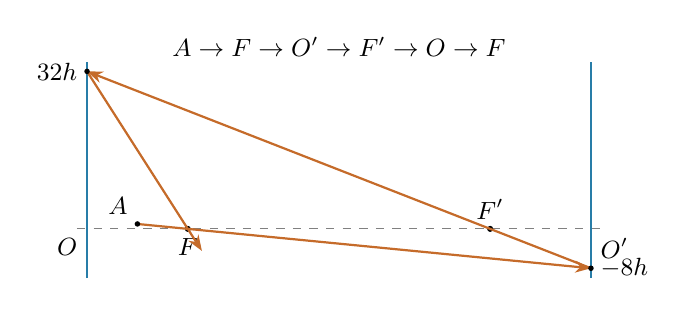
\begin{tikzpicture}[x=.64cm,y=.0625cm]
  \draw[helper] (-.2,0)--(10.3,0);
  \draw[field,thick] (0,-10)--(0,34);\draw[field,thick] (10,-10)--(10,34);
  \fill (2,0) circle (1.1pt) node[below] {$F$};\fill (8,0) circle (1.1pt) node[above] {$F'$};
  \node[below left] at (0,0) {$O$};\node[below right] at (10,0) {$O'$};
  \draw[vec,force] (1,1)--(10,-8);
  \draw[vec,force] (10,-8)--(0,32);
  \draw[vec,force] (0,32)--(2.28,-4.48);
  \fill (1,1) circle (1pt) node[above left] {$A$};
  \fill (10,-8) circle (1pt) node[right] {$-8h$};
  \fill (0,32) circle (1pt) node[left] {$32h$};
  \node at (5,37) {$A\to F\to O'\to F'\to O\to F$};
\end{tikzpicture}
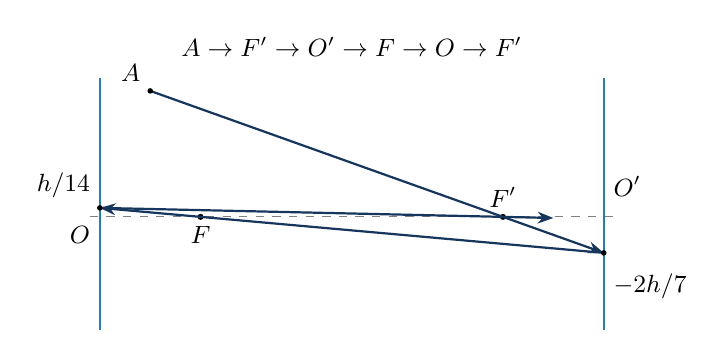
\begin{tikzpicture}[x=.64cm,y=1.6cm]
  \axisray
  \draw[vec,ink] (1,1)--(10,{-2/7});
  \draw[vec,ink] (10,{-2/7})--(0,{1/14});
  \draw[vec,ink] (0,{1/14})--(9,{-1/112});
  \fill (1,1) circle (1pt) node[above left] {$A$};
  \fill (10,{-2/7}) circle (1pt) node[below right,yshift=-4pt] {$-2h/7$};
  \fill (0,{1/14}) circle (1pt) node[above left] {$h/14$};
  \node at (5,1.35) {$A\to F'\to O'\to F\to O\to F'$};
\end{tikzpicture}
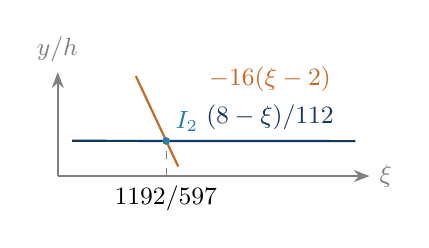
\begin{tikzpicture}[x=180cm,y=24cm]
  \draw[vec,gray] (1.989,.035)--(2.011,.035) node[right] {$\xi$};
  \draw[vec,gray] (1.989,.035)--(1.989,.09) node[above] {$y/h$};
  \draw[force,thick,domain=1.9945:1.9975,samples=2] plot (\x,{-16*(\x-2)});
  \draw[ink,thick,domain=1.99:2.01,samples=2] plot (\x,{(8-\x)/112});
  \fill[field] ({1192/597},{32/597}) circle (1.4pt);
  \draw[helper] ({1192/597},.035)--({1192/597},{32/597});
  \node[below] at ({1192/597},.035) {$1192/597$};
  \node[field,above right] at ({1192/597},{32/597}) {$I_2$};
  \node[force] at (2.004,.086) {$-16(\xi-2)$};
  \node[ink] at (2.004,.066) {$(8-\xi)/112$};
\end{tikzpicture}
\end{document}
